\documentclass[10pt,letterpaper]{article}
\usepackage{iftex}
\ifPDFTeX
\usepackage[utf8]{inputenc}
\usepackage[T1]{fontenc}
\usepackage{lmodern}
\usepackage[sfdefault,lf]{carlito}
\renewcommand*\familydefault{\sfdefault}
\else
\usepackage{fontspec}
\IfFontExistsTF{Calibri}{\setmainfont{Calibri}}{\setmainfont{Carlito}}
\fi
\usepackage[spanish,es-tabla,es-noshorthands]{babel}
\usepackage{geometry}
\usepackage{graphicx}
\usepackage[table]{xcolor}
\usepackage{tabularx}
\usepackage{array}
\usepackage{longtable}
\usepackage{pdflscape}
\usepackage{setspace}
\usepackage{float}
\usepackage{caption}
\usepackage{enumitem}
\usepackage{newunicodechar}
\usepackage{titlesec}
\usepackage{xurl}
\usepackage{hyperref}
\urlstyle{same}
\geometry{margin=1.9cm}
\setstretch{1.15}
\ifPDFTeX\else
\newunicodechar{→}{\ensuremath{\to}}
\newunicodechar{×}{\ensuremath{\times}}
\fi
\newunicodechar{≤}{\ensuremath{\leq}}
\newunicodechar{≥}{\ensuremath{\geq}}
\newunicodechar{−}{\ensuremath{-}}
\definecolor{tecAzul}{HTML}{1F4E9A}
\hypersetup{colorlinks=true, linkcolor=blue, urlcolor=blue}
\captionsetup{font=small, skip=4pt}
\setlength{\parskip}{0.3em}
\setlength{\intextsep}{6pt}
\titleformat{\section}{\large\bfseries}{\thesection.}{0.5em}{}
\titlespacing*{\section}{0pt}{8pt}{3pt}
\titleformat{\subsection}{\normalsize\bfseries}{\thesubsection.}{0.5em}{}
\titlespacing*{\subsection}{0pt}{6pt}{2pt}
\titleformat{\paragraph}[runin]{\normalsize\bfseries}{}{0em}{}
\setlength{\parindent}{0pt}
\setlist[itemize]{nosep, leftmargin=1.2em, label=\textbullet}
\setlist[enumerate]{nosep, leftmargin=1.5em}
\graphicspath{{figuras/}}
\setcounter{tocdepth}{2}
\newcolumntype{L}{>{\raggedright\arraybackslash}X}
\newcolumntype{P}[1]{>{\raggedright\arraybackslash\hspace{0pt}}p{#1}}
\newcolumntype{C}[1]{>{\centering\arraybackslash}p{#1}}
\renewcommand{\arraystretch}{1.0}
\setlength{\tabcolsep}{4pt}
\setlength{\LTpre}{4pt}
\setlength{\LTpost}{6pt}

\begin{document}

\begin{minipage}[c]{0.27\textwidth}
\includegraphics[width=\textwidth]{\detokenize{Logo-unab.svg.png}}
\end{minipage}\hfill
\begin{minipage}[c]{0.7\textwidth}
\small
Facultad de Ingeniería

Desarrollo Web y Móvil

Evaluación de la Unidad 2: \textbf{Diseño e implementación de un backend seguro completo}

Caso N.° 15: \textbf{Mr. Sandwich}, venta de sándwiches, hamburguesas, promociones y bebidas con retiro o delivery
\end{minipage}

\begin{center}
\footnotesize
\begin{tabularx}{\textwidth}{|P{0.16\textwidth}|L|P{0.13\textwidth}|L|}
\hline
\textbf{Campo} & \textbf{Datos} & \textbf{Campo} & \textbf{Datos} \\ \hline
Integrantes & Max Fernández, Tomás Hurtado & Fecha & 09-11-2026 \\ \hline
Docente & \textit Ernesto Vivanco & NRC & \textit 8478 \\ \hline
Versión del frontend & Commit 6aa8c51 del 26-10-2026, carpeta \textit{proyecto backend y front end/frontend} & Repositorio & \url{https://github.com/Makkusu88/Desarrollo-web-y-movil} \\ \hline
\multicolumn{4}{|p{\dimexpr\textwidth-2\tabcolsep-0.8pt\relax}|}{\textbf{Ejecución:} el sistema completo se inicia con \texttt{python run\_all.py --reset}. Las instrucciones, dependencias, pruebas y evidencias están en el repositorio.} \\ \hline
\end{tabularx}
\end{center}

{\small\setstretch{1.0}\tableofcontents}
\newpage


\section*{Introducción}\phantomsection\addcontentsline{toc}{section}{Introducción}
Este informe presenta el trabajo que realizamos para el caso N.° 15, Mr. Sandwich, una aplicación de venta de sándwiches, hamburguesas, promociones y bebidas, con opción de retiro o entrega a domicilio. La actividad consiste en diseñar un backend seguro que se comunique con el frontend del proyecto.

Nuestro punto de partida fue una interfaz con menú, detalle de productos y una simulación de inicio de sesión. El desafío fue transformar esas pantallas en un sistema que pudiera consultar y guardar información de verdad, registrar clientes, controlar pedidos y validar los pagos sin confiar en datos modificables desde el navegador.


\subsection*{Objetivo general}\phantomsection\addcontentsline{toc}{subsection}{Objetivo general}
Diseñar y documentar un backend para Mr. Sandwich, integrado con el frontend, que considere las funciones del negocio y aplique controles de acceso, separación de servicios y protección de datos.


\subsection*{Objetivos específicos}\phantomsection\addcontentsline{toc}{subsection}{Objetivos específicos}
Identificar los servicios que necesita cada pantalla modelar las entidades y sus relaciones, organizar inventory, orders, clients y payments, definir rutas y permisos, proteger las credenciales y datos personales, y documentar la integración, las pruebas y las limitaciones del proyecto.


\subsection*{Requisitos del caso}\phantomsection\addcontentsline{toc}{subsection}{Requisitos del caso}
Primero identificamos las funciones que debía cumplir la aplicación de Mr. Sandwich. En esta tabla presentamos los requisitos del negocio. Más adelante explicamos las decisiones técnicas que utilizamos para implementarlos.

{\footnotesize
\begin{longtable}{|P{\dimexpr 0.2330\linewidth-2\tabcolsep\relax}|P{\dimexpr 0.7520\linewidth-2\tabcolsep\relax}|}
\hline
\textbf{ID} & \textbf{Requisito} \\ \hline
\endfirsthead
\hline
\textbf{ID} & \textbf{Requisito} \\ \hline
\endhead
RF01 & Ver el menú catálogo por categoría y buscar productos \\ \hline
RF02 & Ver el detalle de un producto y personalizarlo  \\ \hline
RF03 & Registrarse e iniciar o cerrar sesión \\ \hline
RF04 & Recuperar la contraseña olvidada \\ \hline
RF05 & Armar un pedido con el carrito y conocer el precio oficial antes de confirmar \\ \hline
RF06 & Confirmar el pedido para retiro o delivery a una dirección propia \\ \hline
RF07 & Pagar el pedido en línea \\ \hline
RF08 & Seguir el estado del pedido y consultar el historial \\ \hline
RF09 & Administrar perfil y direcciones de entrega \\ \hline
RF10 & El Personal preparara y despacha pedidos cambiando su estado \\ \hline
RF11 & El Administrador administra productos, precios, disponibilidad y stock \\ \hline
RF12 & El Administrador consulta reportes de ventas y alertas de stock bajo \\ \hline
RF13 & Anular un pedido no pagado o uno pagado con reembolso \\ \hline
\end{longtable}}

\paragraph{Pantallas}\mbox{}\\[2pt]
{\footnotesize
\begin{longtable}{|P{\dimexpr 0.4917\linewidth-2\tabcolsep\relax}|P{\dimexpr 0.4933\linewidth-2\tabcolsep\relax}|}
\hline
\textbf{Pantalla} & \textbf{Archivo} \\ \hline
\endfirsthead
\hline
\textbf{Pantalla} & \textbf{Archivo} \\ \hline
\endhead
P01 Catálogo & index.\allowbreak{}html \\ \hline
P02 Detalle & producto.\allowbreak{}html \\ \hline
P03 Login & login.\allowbreak{}html \\ \hline
P04 Registro & registro.\allowbreak{}html \\ \hline
P05 Carrito & carrito.\allowbreak{}html \\ \hline
P06 Seguimiento & pedido.\allowbreak{}html \\ \hline
P07 Mi cuenta & cuenta.\allowbreak{}html \\ \hline
P08 Recuperar contraseña & restablecer.\allowbreak{}html \\ \hline
P09 Panel del local & admin.\allowbreak{}html \\ \hline
P10 Página de pago & (proveedor) \\ \hline
\end{longtable}}

\subsection*{Brechas declaradas}\phantomsection\addcontentsline{toc}{subsection}{Brechas declaradas}
Estas son las partes del caso que no quedaron completas o que resolvimos con una alternativa de prueba. Las dejamos declaradas para que no se confundan con funciones terminadas. El detalle está en el módulo 10.

{\footnotesize
\begin{longtable}{|P{\dimexpr 0.2189\linewidth-2\tabcolsep\relax}|P{\dimexpr 0.0958\linewidth-2\tabcolsep\relax}|P{\dimexpr 0.3694\linewidth-2\tabcolsep\relax}|P{\dimexpr 0.3010\linewidth-2\tabcolsep\relax}|}
\hline
\textbf{Brecha} & \textbf{Requisito} & \textbf{Qué hicimos} & \textbf{Qué falta} \\ \hline
\endfirsthead
\hline
\textbf{Brecha} & \textbf{Requisito} & \textbf{Qué hicimos} & \textbf{Qué falta} \\ \hline
\endhead
Recuperación de contraseña sin envío de correo & RF04 & El correo con el enlace se guarda como archivo .eml en la carpeta de ejecución & Conectar un servidor de correo real \\ \hline
Pago con proveedor de prueba & RF07 & provider\_\allowbreak{}sim mantiene el contrato del proveedor: sesión de pago, clave de API y webhook firmado & Conectar el entorno de pruebas de un proveedor real \\ \hline
Reembolso no ejecutado & RF13 & Un pedido pagado que el administrador anula queda marcado como requiere\_\allowbreak{}reembolso & Ejecutar la devolución del dinero con el proveedor \\ \hline
Vault en modo desarrollo & — & Los secretos se generan en cada arranque y cada servicio solo lee los suyos & Un Vault persistente, hoy los secretos se pierden al detener el sistema \\ \hline
Sin HTTPS entre el navegador y el gateway & — & Todo corre en localhost, la comunicación gRPC interna sí usa mTLS & Certificados HTTPS para el frontend y el API Gateway \\ \hline
Todo en un solo computador & — & La separación pública y privada se hace escuchando en 127.0.0.1 y con run\_\allowbreak{}all.\allowbreak{}py & Probar el sistema repartido en varias máquinas o contenedores \\ \hline
\end{longtable}}

\section*{Módulo 1 Servicios derivados del frontend}\phantomsection\addcontentsline{toc}{section}{Módulo 1 Servicios derivados del frontend}
En este módulo relacionamos las acciones de cada pantalla con los servicios del backend. Decidimos que el navegador no pueda fijar los precios ni dar por aprobado un pago, el backend comprueba esos datos y calcula el total usando la información oficial de inventario.

\begin{landscape}

\subsection*{1.1 Catálogo de servicios}\phantomsection\addcontentsline{toc}{subsection}{1.1 Catálogo de servicios}
{\scriptsize
\begin{longtable}{|P{\dimexpr 0.0471\linewidth-2\tabcolsep\relax}|P{\dimexpr 0.0512\linewidth-2\tabcolsep\relax}|P{\dimexpr 0.1291\linewidth-2\tabcolsep\relax}|P{\dimexpr 0.1310\linewidth-2\tabcolsep\relax}|P{\dimexpr 0.1235\linewidth-2\tabcolsep\relax}|P{\dimexpr 0.1424\linewidth-2\tabcolsep\relax}|P{\dimexpr 0.1139\linewidth-2\tabcolsep\relax}|P{\dimexpr 0.1139\linewidth-2\tabcolsep\relax}|P{\dimexpr 0.0664\linewidth-2\tabcolsep\relax}|P{\dimexpr 0.0665\linewidth-2\tabcolsep\relax}|}
\hline
\textbf{ID} & \textbf{Requisito} & \textbf{Pantalla y acción} & \textbf{¿Para qué sirve?\allowbreak{}} & \textbf{Método y ruta de la API} & \textbf{¿Qué recibe?\allowbreak{}} & \textbf{¿Qué devuelve?\allowbreak{}} & \textbf{Reglas y posibles errores} & \textbf{Tipo de dato} & \textbf{¿Quién puede usarlo?\allowbreak{}} \\ \hline
\endfirsthead
\hline
\textbf{ID} & \textbf{Requisito} & \textbf{Pantalla y acción} & \textbf{¿Para qué sirve?\allowbreak{}} & \textbf{Método y ruta de la API} & \textbf{¿Qué recibe?\allowbreak{}} & \textbf{¿Qué devuelve?\allowbreak{}} & \textbf{Reglas y posibles errores} & \textbf{Tipo de dato} & \textbf{¿Quién puede usarlo?\allowbreak{}} \\ \hline
\endhead
\textbf{S01} & RF01 & P01: abrir el menú & Muestra los productos del local. & GET /\allowbreak{}api/\allowbreak{}v1/\allowbreak{}products?\allowbreak{}available\&\allowbreak{}category\&\allowbreak{}q\&\allowbreak{}limit\&\allowbreak{}offset & Filtros opcionales: disponible, categoría, búsqueda (hasta 40 caracteres), límite (1–100) y desde qué resultado empezar. & 200: lista de productos, lista vacía si no hay. & 400 si los filtros están mal. Se muestran los productos disponibles. & Público & Cualquiera \\ \hline
\textbf{S01} & RF01 & P01: elegir categoría & Muestra las categorías del menú. & GET /\allowbreak{}api/\allowbreak{}v1/\allowbreak{}categories & No necesita datos. & 200: categorías con ID y nombre. & No se indican errores especiales. & Público & Cualquiera \\ \hline
\textbf{S02} & RF02 & P02: abrir un producto & Muestra su detalle, opciones y extras. & GET /\allowbreak{}api/\allowbreak{}v1/\allowbreak{}products/\allowbreak{}\{id\} & ID numérico del producto. & 200: datos del producto, opciones y extras. & 404 si el producto no existe o fue dado de baja. & Público & Cualquiera \\ \hline
\textbf{S03} & RF03 & P04: registrarse & Crea una cuenta con el perfil del cliente. & POST /\allowbreak{}api/\allowbreak{}v1/\allowbreak{}auth/\allowbreak{}register & Nombre (2–60 letras o caracteres), correo válido, contraseña de al menos 8 caracteres con letras y números; teléfono opcional (8 a 12 dígitos, con “+” opcional). & 201: ID del usuario y correo. & 409 si el correo ya existe 400 si la clave no cumple 503 si falla el sistema de clientes y se revierte el registro. & Credencial y privado & Sin cuenta; con límite de intentos \\ \hline
\textbf{S04} & RF03 & P03: iniciar sesión & Comprueba correo y contraseña. & POST /\allowbreak{}api/\allowbreak{}v1/\allowbreak{}auth/\allowbreak{}login & Correo y contraseña. & 200: ID, roles, duración y cookie segura ms\_\allowbreak{}session (HttpOnly, SameSite=Strict). & 401 si no coincide, 429 si hubo 5 fallos o demasiados intentos. & Credencial & Sin cuenta, con límite de intentos \\ \hline
\textbf{S05} & RF03 & P07/\allowbreak{}P09: cerrar sesión & Cierra la sesión activa. & POST /\allowbreak{}api/\allowbreak{}v1/\allowbreak{}auth/\allowbreak{}logout & Cookie de sesión. & 200: sesión cerrada y cookie eliminada. & 401 si no hay una sesión válida. & Credencial & Usuario con sesión \\ \hline
\textbf{S06} & RF04 & P08: pedir enlace & Solicita recuperar la contraseña. & POST /\allowbreak{}api/\allowbreak{}v1/\allowbreak{}auth/\allowbreak{}password-reset/\allowbreak{}request & Correo electrónico. & 202: responde lo mismo tanto si existe la cuenta como si no. & No revela si un correo está registrado. & Privado & Cualquiera, con límite de intentos \\ \hline
\textbf{S07} & RF04 & P08: guardar clave nueva & Cambia la contraseña usando un enlace válido. & POST /\allowbreak{}api/\allowbreak{}v1/\allowbreak{}auth/\allowbreak{}password-reset/\allowbreak{}confirm & Token de recuperación y contraseña nueva. & 200: clave cambiada. & 400 si el token venció o ya se usó, cierra sesiones anteriores. & Credencial & Quien tenga el token de un solo uso \\ \hline
\textbf{S09} & RF09 & P07: abrir mi cuenta & Muestra los datos del cliente conectado. & GET /\allowbreak{}api/\allowbreak{}v1/\allowbreak{}clients/\allowbreak{}me & No necesita datos extra. & 200: ID, nombre, correo y teléfono. & 401 si no ha iniciado sesión. & Privado & Usuario con sesión \\ \hline
\textbf{S10} & RF09 & P07: guardar mi perfil & Actualiza el nombre y el teléfono. & PUT /\allowbreak{}api/\allowbreak{}v1/\allowbreak{}clients/\allowbreak{}me & Nombre, teléfono opcional. & 200: perfil actualizado. & 400 si los datos ingresados son incorrectos. & Privado & Usuario con sesión \\ \hline
\textbf{S11} & RF06/\allowbreak{}RF09 & P05/\allowbreak{}P07: ver direcciones & Lista las direcciones del cliente. & GET /\allowbreak{}api/\allowbreak{}v1/\allowbreak{}clients/\allowbreak{}me/\allowbreak{}addresses & No necesita datos extra. & 200: lista de sus direcciones. & Solo se consultan las direcciones propias. & Privado & Usuario con sesión \\ \hline
\textbf{S12} & RF09 & P07: agregar dirección & Guarda una nueva dirección de entrega. & POST /\allowbreak{}api/\allowbreak{}v1/\allowbreak{}clients/\allowbreak{}me/\allowbreak{}addresses & Nombre de la dirección, calle, número, comuna, referencia opcional. & 201: dirección creada. & 409 si ya tiene 5 direcciones. & Privado & Usuario con sesión \\ \hline
\textbf{S13} & RF09 & P07: editar dirección & Cambia una dirección ya guardada. & PUT /\allowbreak{}api/\allowbreak{}v1/\allowbreak{}clients/\allowbreak{}me/\allowbreak{}addresses/\allowbreak{}\{id\} & ID de dirección y los mismos campos de S12. & 200: dirección actualizada. & 404 si no es una dirección del usuario. & Privado & Usuario con sesión \\ \hline
\textbf{S14} & RF09 & P07: eliminar dirección & Borra una dirección de la cuenta. & DELETE /\allowbreak{}api/\allowbreak{}v1/\allowbreak{}clients/\allowbreak{}me/\allowbreak{}addresses/\allowbreak{}\{id\} & ID de la dirección. & 204: dirección eliminada. & 404 si no es propia. Los pedidos anteriores conservan la dirección usada. & Privado & Usuario con sesión \\ \hline
\textbf{S15} & RF05 & P05: ver el total & Calcula el precio oficial antes de comprar, sin descontar stock. & POST /\allowbreak{}api/\allowbreak{}v1/\allowbreak{}orders/\allowbreak{}quote & Productos y cantidades (1–10 por ítem), hasta 20 ítems; opciones y extras opcionales (0–5 por extra). & 200: productos, extras, precio por unidad, total de cada ítem y subtotal. & 400 si la opción o el extra es inválido; 409 si no está disponible. & Público & Cualquiera \\ \hline
\textbf{S16} & RF06 & P05: confirmar compra & Crea el pedido y reserva los productos. & POST /\allowbreak{}api/\allowbreak{}v1/\allowbreak{}orders + Idempotency-Key & Ítems como S15, retiro o delivery, ID de dirección si corresponde y notas de hasta 140 caracteres. Incluye Idempotency-Key para evitar pedidos duplicados. & 201: pedido pendiente de pago, con hora de vencimiento. & 409 sin stock o si ya hay más de 3 pedidos pendientes, 404 dirección ajena, 503 si falla inventario: no guarda el pedido. & Privado & Cliente conectado \\ \hline
\textbf{S17} & RF08 & P07: ver mis pedidos & Muestra las compras anteriores del cliente. & GET /\allowbreak{}api/\allowbreak{}v1/\allowbreak{}orders/\allowbreak{}me?\allowbreak{}limit\&\allowbreak{}offset & Cantidad por página (1–20) y desplazamiento. & 200: pedidos y cantidad total. & Solo muestra pedidos del usuario. & Privado & Usuario con sesión \\ \hline
\textbf{S18} & RF08 & P06: abrir un pedido & Muestra toda la información de un pedido. & GET /\allowbreak{}api/\allowbreak{}v1/\allowbreak{}orders/\allowbreak{}\{id\} & ID del pedido. & 200: detalle del pedido. & 404 si es de otra persona, no informa si existe. & Privado & Dueño o trabajador autorizado \\ \hline
\textbf{S19} & RF13 & P06/\allowbreak{}P09: anular pedido & Cancela el pedido sin borrar su historial. & POST /\allowbreak{}api/\allowbreak{}v1/\allowbreak{}orders/\allowbreak{}\{id\}/\allowbreak{}cancel & ID del pedido. & 200: pedido con estado ANULADO. & 409 si el estado no permite anularlo. Libera stock, si estaba pagado, queda marcado para reembolso. & Privado & Dueño, si está pendiente, o administrador \\ \hline
\textbf{S20} & RF10 & P09: ver pedidos del local & Muestra los pedidos que atiende el negocio. & GET /\allowbreak{}api/\allowbreak{}v1/\allowbreak{}orders?\allowbreak{}estado & Filtro de estado opcional. & 200: pedidos, total y contacto necesario para atenderlos. & 403 si intenta entrar un cliente común. & Privado & Personal o administrador \\ \hline
\textbf{S21} & RF10 & P09: cambiar estado & Avanza el pedido en la preparación o entrega. & PUT /\allowbreak{}api/\allowbreak{}v1/\allowbreak{}orders/\allowbreak{}\{id\}/\allowbreak{}status & ID y nuevo estado: en preparacion, listo, en reparto o entregado. & 200: pedido actualizado. & 409 si el cambio no está permitido. No se acepta pagado como estado desde aquí. & Privado & Personal o administrador \\ \hline
\textbf{S22} & RF07 & P05/\allowbreak{}P06: pagar pedido & Inicia el pago con el proveedor. & POST /\allowbreak{}api/\allowbreak{}v1/\allowbreak{}payments & ID del pedido (order\_\allowbreak{}id). & 201: ID del pago, estado, monto y enlace para pagar. & 409 si el pedido no espera pago, reutiliza un intento existente, 503 si falla el proveedor. & Privado & Cliente dueño del pedido \\ \hline
\textbf{S23} & RF07/\allowbreak{}RF08 & P06: revisar pago & Consulta el último intento de pago. & GET /\allowbreak{}api/\allowbreak{}v1/\allowbreak{}payments/\allowbreak{}order/\allowbreak{}\{id\} & ID del pedido. & 200: información del pago. & 404 si no existe o no pertenece al usuario. & Privado & Dueño o personal autorizado \\ \hline
\textbf{S24} & RF07 & Proveedor: avisar el pago & Recibe la confirmación de pago del proveedor. & POST /\allowbreak{}api/\allowbreak{}v1/\allowbreak{}payments/\allowbreak{}webhook & Datos del proveedor y firma con fecha. & 200: aviso recibido y resultado indica si era repetido. & 401 si la firma no es válida o tiene más de 300 segundos. & Privado & Solo proveedor con firma válida \\ \hline
\textbf{S25} & RF11 & P09: ver productos & Muestra productos y existencias del local. & GET /\allowbreak{}api/\allowbreak{}v1/\allowbreak{}admin/\allowbreak{}products & No necesita datos. & 200: productos, stock y mínimo permitido. & 403 si entra un cliente común. & Privado del negocio & Personal o administrador \\ \hline
\textbf{S26} & RF11 & P09: crear producto & Agrega un producto al catálogo. & POST /\allowbreak{}api/\allowbreak{}v1/\allowbreak{}admin/\allowbreak{}products & Nombre, categoría, precio entre 100 y 100000, descripción, imagen permitida, disponibilidad, stock y stock mínimo. & 201: producto creado. & 400 si categoría o imagen no son válidas. & Público y privado & Solo administrador \\ \hline
\textbf{S27} & RF11 & P09: editar producto & Cambia los datos de un producto. & PUT /\allowbreak{}api/\allowbreak{}v1/\allowbreak{}admin/\allowbreak{}products/\allowbreak{}\{id\} & ID del producto y los mismos datos que S26. & 200: producto actualizado. & 404 si el producto no existe. & Público y privado & Solo administrador \\ \hline
\textbf{S28} & RF11 & P09: dar de baja & Oculta un producto sin borrarlo del historial. & DELETE /\allowbreak{}api/\allowbreak{}v1/\allowbreak{}admin/\allowbreak{}products/\allowbreak{}\{id\} & ID del producto. & 204: producto dado de baja. & 404 si no existe, los pedidos antiguos conservan ese producto. & No aplica & Solo administrador \\ \hline
\textbf{S29} & RF11 & P09: actualizar stock & Cambia la cantidad disponible. & PUT /\allowbreak{}api/\allowbreak{}v1/\allowbreak{}admin/\allowbreak{}products/\allowbreak{}\{id\}/\allowbreak{}stock & ID del producto y stock entre 0 y 10000. & 200: stock actualizado. & 404 si el producto no existe. & Privado del negocio & Personal o administrador \\ \hline
\textbf{S30} & RF08/\allowbreak{}RF10/\allowbreak{}RF12 & P06/\allowbreak{}P07/\allowbreak{}P09: ver resúmenes & Reúne datos de varios sistemas en una sola consulta. & POST /\allowbreak{}api/\allowbreak{}v1/\allowbreak{}graphql & Consulta GraphQL & 200: datos pedidos y, si corresponde, errores parciales. & Comprueba permisos por consulta y campo, limita consultas demasiado grandes o profundas. & Privado & Usuario con sesión y permisos \\ \hline
\textbf{S31} &  & Todas: mostrar sesión & Permite saber si hay sesión para mostrar los menús correctos. & GET /\allowbreak{}api/\allowbreak{}v1/\allowbreak{}session & Cookie de sesión, si existe. & 200: indica si inició sesión, su ID y roles cuando corresponda. & Solo ayuda a mostrar la interfaz, no da permisos por sí mismo. & Privado & Cualquiera \\ \hline
\end{longtable}}
\end{landscape}

\subsection*{1.2 Ejemplos de contratos con datos ficticios}\phantomsection\addcontentsline{toc}{subsection}{1.2 Ejemplos de contratos con datos ficticios}
\textbf{S01} GET /\allowbreak{}api/\allowbreak{}v1/\allowbreak{}products?\allowbreak{}category=bebidas

{\footnotesize\ttfamily\raggedright\setlength{\parskip}{0pt}
[\{\textquotedbl{}id\textquotedbl{}: 9, \textquotedbl{}nombre\textquotedbl{}: \textquotedbl{}Coca-Cola 350 ml\textquotedbl{}, \textquotedbl{}categoria\textquotedbl{}: \textquotedbl{}bebidas\textquotedbl{}, \textquotedbl{}precio\textquotedbl{}: 1990,\par
\textquotedbl{}descripcion\textquotedbl{}: \textquotedbl{}Bebida Coca-Cola en lata, bien helada.\textquotedbl{}, \textquotedbl{}imagen\textquotedbl{}: \textquotedbl{}img/\allowbreak{}bebida.\allowbreak{}svg\textquotedbl{}, \textquotedbl{}disponible\textquotedbl{}: true\}]\par}

\textbf{S15} POST /\allowbreak{}api/\allowbreak{}v1/\allowbreak{}orders/\allowbreak{}quote. En este ejemplo mostramos que un precio enviado por el navegador, incluso si fue cambiado intencionalmente, no se utiliza para calcular la cotización del pedido:

{\footnotesize\ttfamily\raggedright\setlength{\parskip}{0pt}
\{\textquotedbl{}items\textquotedbl{}: [\{\textquotedbl{}product\_\allowbreak{}id\textquotedbl{}: 1, \textquotedbl{}option\_\allowbreak{}id\textquotedbl{}: \textquotedbl{}grande\textquotedbl{}, \textquotedbl{}extras\textquotedbl{}: [\{\textquotedbl{}extra\_\allowbreak{}id\textquotedbl{}: \textquotedbl{}palta\textquotedbl{}, \textquotedbl{}qty\textquotedbl{}: 2\}], \textquotedbl{}qty\textquotedbl{}: 2, \textquotedbl{}precio\_\allowbreak{}unitario\textquotedbl{}: 1\}]\}\par}

{\footnotesize\ttfamily\raggedright\setlength{\parskip}{0pt}
\{\textquotedbl{}items\textquotedbl{}: [\{\textquotedbl{}product\_\allowbreak{}id\textquotedbl{}: 1, \textquotedbl{}nombre\textquotedbl{}: \textquotedbl{}Churrasco italiano\textquotedbl{}, \textquotedbl{}opcion\textquotedbl{}: \textquotedbl{}Tamaño grande\textquotedbl{}, \textquotedbl{}extras\textquotedbl{}: [\textquotedbl{}Palta extra x2\textquotedbl{}],\par
\textquotedbl{}qty\textquotedbl{}: 2, \textquotedbl{}precio\_\allowbreak{}unitario\textquotedbl{}: 10090, \textquotedbl{}total\_\allowbreak{}linea\textquotedbl{}: 20180\}], \textquotedbl{}subtotal\textquotedbl{}: 20180\}\par}

\textbf{S16} POST /\allowbreak{}api/\allowbreak{}v1/\allowbreak{}orders con Idempotency-Key: 6f1c…

{\footnotesize\ttfamily\raggedright\setlength{\parskip}{0pt}
\{\textquotedbl{}items\textquotedbl{}: [\{\textquotedbl{}product\_\allowbreak{}id\textquotedbl{}: 6, \textquotedbl{}option\_\allowbreak{}id\textquotedbl{}: \textquotedbl{}doble\textquotedbl{}, \textquotedbl{}extras\textquotedbl{}: [\{\textquotedbl{}extra\_\allowbreak{}id\textquotedbl{}: \textquotedbl{}tocino\textquotedbl{}, \textquotedbl{}qty\textquotedbl{}: 1\}], \textquotedbl{}qty\textquotedbl{}: 1\}],\par
\textquotedbl{}tipo\_\allowbreak{}entrega\textquotedbl{}: \textquotedbl{}DELIVERY\textquotedbl{}, \textquotedbl{}direccion\_\allowbreak{}id\textquotedbl{}: \textquotedbl{}DIR-a000000001\textquotedbl{}, \textquotedbl{}notas\textquotedbl{}: \textquotedbl{}Sin cebolla\textquotedbl{}\}\par}

{\footnotesize\ttfamily\raggedright\setlength{\parskip}{0pt}
\{\textquotedbl{}id\textquotedbl{}: \textquotedbl{}PED-02EBEF86\textquotedbl{}, \textquotedbl{}estado\textquotedbl{}: \textquotedbl{}PENDIENTE\_\allowbreak{}PAGO\textquotedbl{}, \textquotedbl{}tipo\_\allowbreak{}entrega\textquotedbl{}: \textquotedbl{}DELIVERY\textquotedbl{},\par
\textquotedbl{}items\textquotedbl{}: [\{\textquotedbl{}product\_\allowbreak{}id\textquotedbl{}: 6, \textquotedbl{}nombre\textquotedbl{}: \textquotedbl{}Hamburguesa clásica\textquotedbl{}, \textquotedbl{}opcion\textquotedbl{}: \textquotedbl{}Carne doble\textquotedbl{}, \textquotedbl{}extras\textquotedbl{}: [\textquotedbl{}Tocino extra x1\textquotedbl{}],\par
\textquotedbl{}qty\textquotedbl{}: 1, \textquotedbl{}precio\_\allowbreak{}unitario\textquotedbl{}: 8380, \textquotedbl{}total\_\allowbreak{}linea\textquotedbl{}: 8380\}],\par
\textquotedbl{}subtotal\textquotedbl{}: 8380, \textquotedbl{}costo\_\allowbreak{}envio\textquotedbl{}: 1990, \textquotedbl{}total\textquotedbl{}: 10370, \textquotedbl{}notas\textquotedbl{}: \textquotedbl{}Sin cebolla\textquotedbl{},\par
\textquotedbl{}creado\_\allowbreak{}en\textquotedbl{}: \textquotedbl{}2026-10-24T20:35:01Z\textquotedbl{}, \textquotedbl{}expira\_\allowbreak{}en\textquotedbl{}: \textquotedbl{}2026-10-24T20:45:01Z\textquotedbl{},\par
\textquotedbl{}direccion\textquotedbl{}: \{\textquotedbl{}id\textquotedbl{}: \textquotedbl{}DIR-a000000001\textquotedbl{}, \textquotedbl{}alias\textquotedbl{}: \textquotedbl{}Casa\textquotedbl{}, \textquotedbl{}calle\textquotedbl{}: \textquotedbl{}Calle Falsa\textquotedbl{}, \textquotedbl{}numero\textquotedbl{}: \textquotedbl{}123\textquotedbl{}, \textquotedbl{}comuna\textquotedbl{}: \textquotedbl{}Santiago\textquotedbl{}, \textquotedbl{}referencia\textquotedbl{}: \textquotedbl{}Depto 4B\textquotedbl{}\},\par
\textquotedbl{}historial\textquotedbl{}: [\{\textquotedbl{}estado\textquotedbl{}: \textquotedbl{}PENDIENTE\_\allowbreak{}PAGO\textquotedbl{}, \textquotedbl{}en\textquotedbl{}: \textquotedbl{}2026-10-24T20:35:01Z\textquotedbl{}\}], \textquotedbl{}requiere\_\allowbreak{}reembolso\textquotedbl{}: false\}\par}

\textbf{S22} POST /\allowbreak{}api/\allowbreak{}v1/\allowbreak{}payments: \{\textquotedbl{}order\_\allowbreak{}id\textquotedbl{}: \textquotedbl{}PED-02EBEF86\textquotedbl{}\}

{\footnotesize\ttfamily\raggedright\setlength{\parskip}{0pt}
\{\textquotedbl{}payment\_\allowbreak{}id\textquotedbl{}: \textquotedbl{}PAY-F47E0DEAC2\textquotedbl{}, \textquotedbl{}order\_\allowbreak{}id\textquotedbl{}: \textquotedbl{}PED-02EBEF86\textquotedbl{}, \textquotedbl{}estado\textquotedbl{}: \textquotedbl{}INICIADO\textquotedbl{}, \textquotedbl{}monto\textquotedbl{}: 10370,\par
\textquotedbl{}comprobante\textquotedbl{}: null, \textquotedbl{}checkout\_\allowbreak{}url\textquotedbl{}: \textquotedbl{}http:/\allowbreak{}/\allowbreak{}localhost:8300/\allowbreak{}checkout/\allowbreak{}cs\_\allowbreak{}128bf58de413f738\textquotedbl{}\}\par}

\textbf{S24} Webhook. Cabecera X-Provider-Signature: t=1792874000,\allowbreak{}v1=<hex HMAC-SHA256(\textquotedbl{}t.\textquotedbl{} + cuerpo)>

{\footnotesize\ttfamily\raggedright\setlength{\parskip}{0pt}
\{\textquotedbl{}id\textquotedbl{}: \textquotedbl{}evt\_\allowbreak{}3a9c…\textquotedbl{}, \textquotedbl{}type\textquotedbl{}: \textquotedbl{}checkout.\allowbreak{}approved\textquotedbl{},\par
\textquotedbl{}data\textquotedbl{}: \{\textquotedbl{}session\_\allowbreak{}id\textquotedbl{}: \textquotedbl{}cs\_\allowbreak{}128bf58de413f738\textquotedbl{}, \textquotedbl{}reference\textquotedbl{}: \textquotedbl{}PAY-F47E0DEAC2\textquotedbl{}, \textquotedbl{}amount\textquotedbl{}: 10370\}\}\par}

También utilizamos un formato de error común. Esto permite que el frontend muestre mensajes entendibles sin entregar información interna del servidor:

{\footnotesize\ttfamily\raggedright\setlength{\parskip}{0pt}
\{\textquotedbl{}error\textquotedbl{}: \{\textquotedbl{}codigo\textquotedbl{}: 404, \textquotedbl{}mensaje\textquotedbl{}: \textquotedbl{}Pedido no encontrado\textquotedbl{}\}, \textquotedbl{}request\_\allowbreak{}id\textquotedbl{}: \textquotedbl{}349a2a2f8a484c93a57793b8343f3311\textquotedbl{}\}\par}


\section*{Módulo 2 Clases y cardinalidades del dominio}\phantomsection\addcontentsline{toc}{section}{Módulo 2 Clases y cardinalidades del dominio}
Para ordenar las clases y sus relaciones preparamos el diagrama UML de dominio. El modelo representa a usuarios, clientes, productos, pedidos, pagos y servicios.

\begin{landscape}
\begin{figure}[H]
\centering
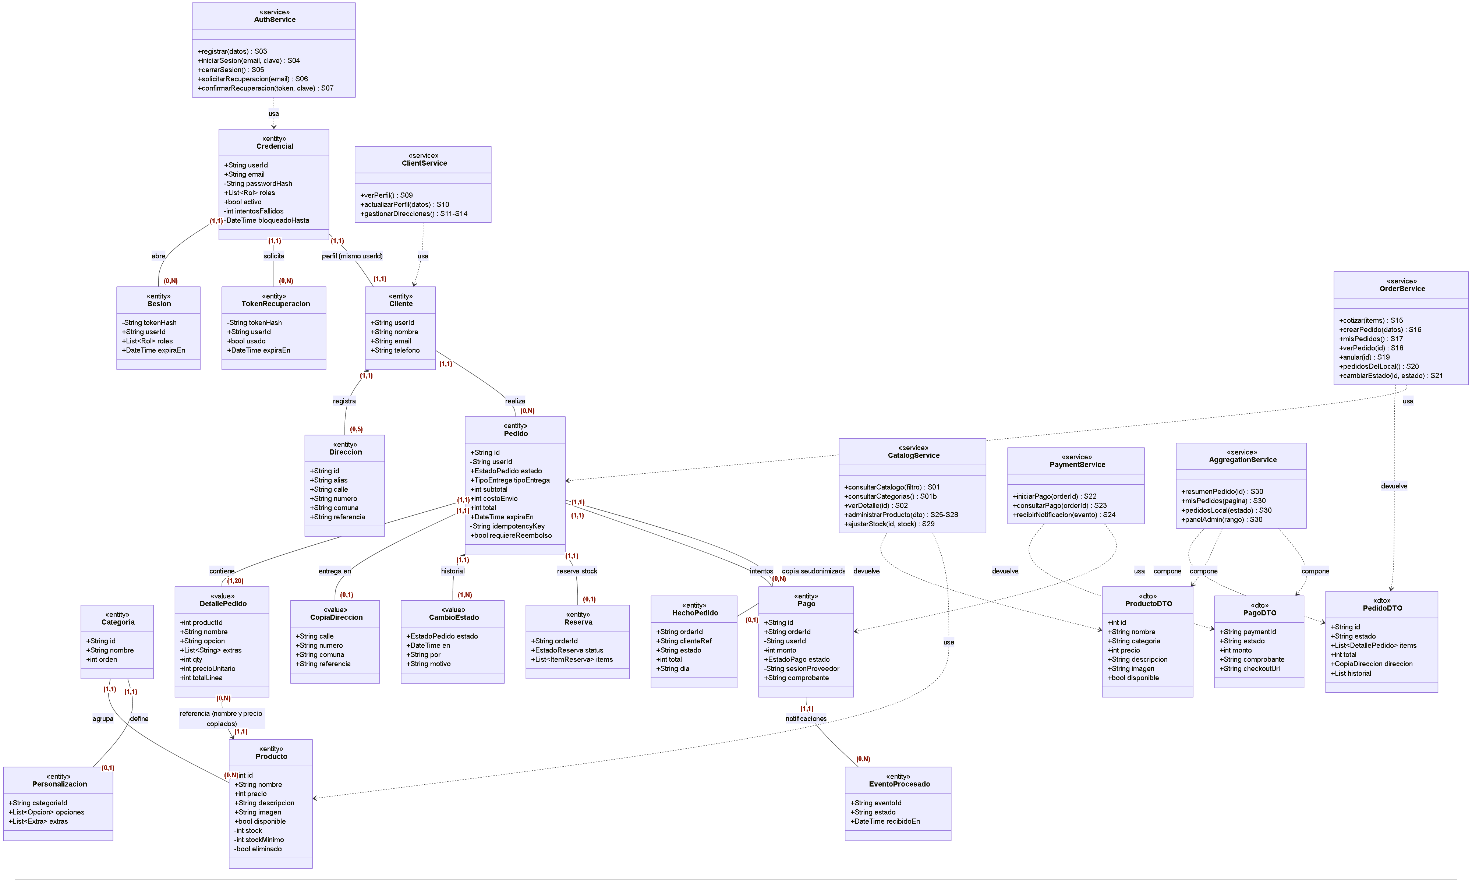
\includegraphics[width=\linewidth,height=0.78\textwidth,keepaspectratio]{uml_dominio.png}
\caption{Diagrama UML de clases del dominio y servicios públicos}
\end{figure}
\end{landscape}

\subsection*{2.1 Relaciones y reglas}\phantomsection\addcontentsline{toc}{subsection}{2.1 Relaciones y reglas}
{\footnotesize
\begin{longtable}{|P{\dimexpr 0.1495\linewidth-2\tabcolsep\relax}|P{\dimexpr 0.1714\linewidth-2\tabcolsep\relax}|P{\dimexpr 0.1579\linewidth-2\tabcolsep\relax}|P{\dimexpr 0.5062\linewidth-2\tabcolsep\relax}|}
\hline
\textbf{Origen} & \textbf{Destino} & \textbf{Cardinalidad} & \textbf{Regla del negocio que la origina} \\ \hline
\endfirsthead
\hline
\textbf{Origen} & \textbf{Destino} & \textbf{Cardinalidad} & \textbf{Regla del negocio que la origina} \\ \hline
\endhead
Credencial & Sesion & 1:N & Un usuario puede tener sesiones en varios dispositivos cada sesión es de un solo usuario \\ \hline
Credencial & TokenRecuperacion & 1:N & Puede pedir varios enlaces cada token es de un usuario y se usa una sola vez \\ \hline
Credencial & Cliente & 1:1 & Toda cuenta tiene un perfil,el registro lo crea si falla, se revierte la credencial \\ \hline
Cliente & Direccion & 1:N & Composición: la dirección no existe sin su cliente máximo 5 para acotar los datos personales guardados \\ \hline
Categoria & Producto & 1:N & Cada producto pertenece a exactamente una categoría del menú \\ \hline
Categoria & Personalizacion & 1:1 & Las opciones y extras se definen por categoría  \\ \hline
Cliente & Pedido & 1:N & Un cliente puede no haber comprado nunca cada pedido tiene un dueño \\ \hline
Pedido & DetallePedido & 1:N & Un pedido confirmado tiene al menos un ítem el límite de 20 líneas evita abusos. No hay borradores vacíos el carrito no se persiste \\ \hline
Pedido & CopiaDireccion & 1:1 & Solo los pedidos delivery tienen dirección es una copia, así que borrar o editar la dirección no altera el historial \\ \hline
Pedido & CambioEstado & 1:N & Todo pedido nace con el evento pendiente a pago y cada transición agrega un evento \\ \hline
DetallePedido & Producto & N:1 & Cada línea referencia un producto, pero copia nombre y precio, si el producto cambia de precio o se da de baja, el historial no cambia \\ \hline
Pedido & Reserva & 1:1 & Un pedido reserva stock una sola vez siendo idempotente por order\_\allowbreak{}id, si la reserva falla, el pedido no se crea \\ \hline
Pedido & Pago & 1:N & Puede haber varios intentos, pero solo uno aprobado con un índice único parcial \\ \hline
Pago & EventoProcesado & 1:N & Cada notificación del proveedor se registra una vez siendo clave = id del evento \\ \hline
Pedido & HechoPedido & 1:1 & La analítica guarda una copia seudonimizada por pedido  \\ \hline
\end{longtable}}

\subsection*{2.2 Decisiones del equipo}\phantomsection\addcontentsline{toc}{subsection}{2.2 Decisiones del equipo}
\begin{itemize}
\item Separamos carrito y pedido porque tienen funciones diferentes. El carrito guarda temporalmente productos y cantidades en el navegador, el pedido se crea cuando el servidor comprueba disponibilidad y precio. De esta manera evitamos confiar en montos almacenados por el usuario.
\item Pensamos también en lo que pasa si un producto deja de venderse. En ese caso conservamos en el detalle del pedido el nombre y el precio registrados al comprar, de modo que el historial no cambie. El producto se da de baja sin eliminar la información de pedidos anteriores.
\item Separamos los datos que el sistema necesita internamente de aquellos que puede mostrar. Por ejemplo, las contraseñas protegidas, el stock interno y las claves de control no aparecen en las respuestas de clientes. La información de contacto de entrega se limita al personal que la necesita.
\end{itemize}

\subsection*{2.3 Operación UML, ID de servicio}\phantomsection\addcontentsline{toc}{subsection}{2.3 Operación UML, ID de servicio}
{\footnotesize
\begin{longtable}{|P{\dimexpr 0.2841\linewidth-2\tabcolsep\relax}|P{\dimexpr 0.7009\linewidth-2\tabcolsep\relax}|}
\hline
\textbf{Servicio UML} & \textbf{Operaciones  ID} \\ \hline
\endfirsthead
\hline
\textbf{Servicio UML} & \textbf{Operaciones  ID} \\ \hline
\endhead
CatalogService & consultarCatalogo a S01,  consultarCategorias a S01b, verDetalle a S02, administrarProducto a S25–S28, ajustarStock a S29 \\ \hline
AuthService & registrar a S03, iniciarSesion a S04, cerrarSesion a S05, solicitarRecuperacion a S06, confirmarRecuperacion a S07 \\ \hline
ClientService & verPerfil a S09, actualizarPerfil a S10, gestionarDirecciones a S11 y S14 \\ \hline
OrderService & cotizar a S15, crearPedido a S16, misPedidos a S17, verPedido a S18, anular a S19, pedidosDelLocal a S20, cambiarEstado a S21 \\ \hline
PaymentService & iniciarPago a S22, consultarPago a S23, recibirNotificacion a S24 \\ \hline
AggregationService & resumenPedido, misPedidos, pedidosLocal, panelAdmin a S30 \\ \hline
\end{longtable}}

\section*{Módulo 3 Sistemas e integraciones}\phantomsection\addcontentsline{toc}{section}{Módulo 3 Sistemas e integraciones}
En esta parte explicamos cómo se conectan los componentes del proyecto. Utilizamos un mapa de arquitectura para mostrar qué sistemas participan y un diagrama de secuencia que sigue una compra con delivery desde el navegador hasta el pago.

\begin{landscape}
\begin{figure}[H]
\centering
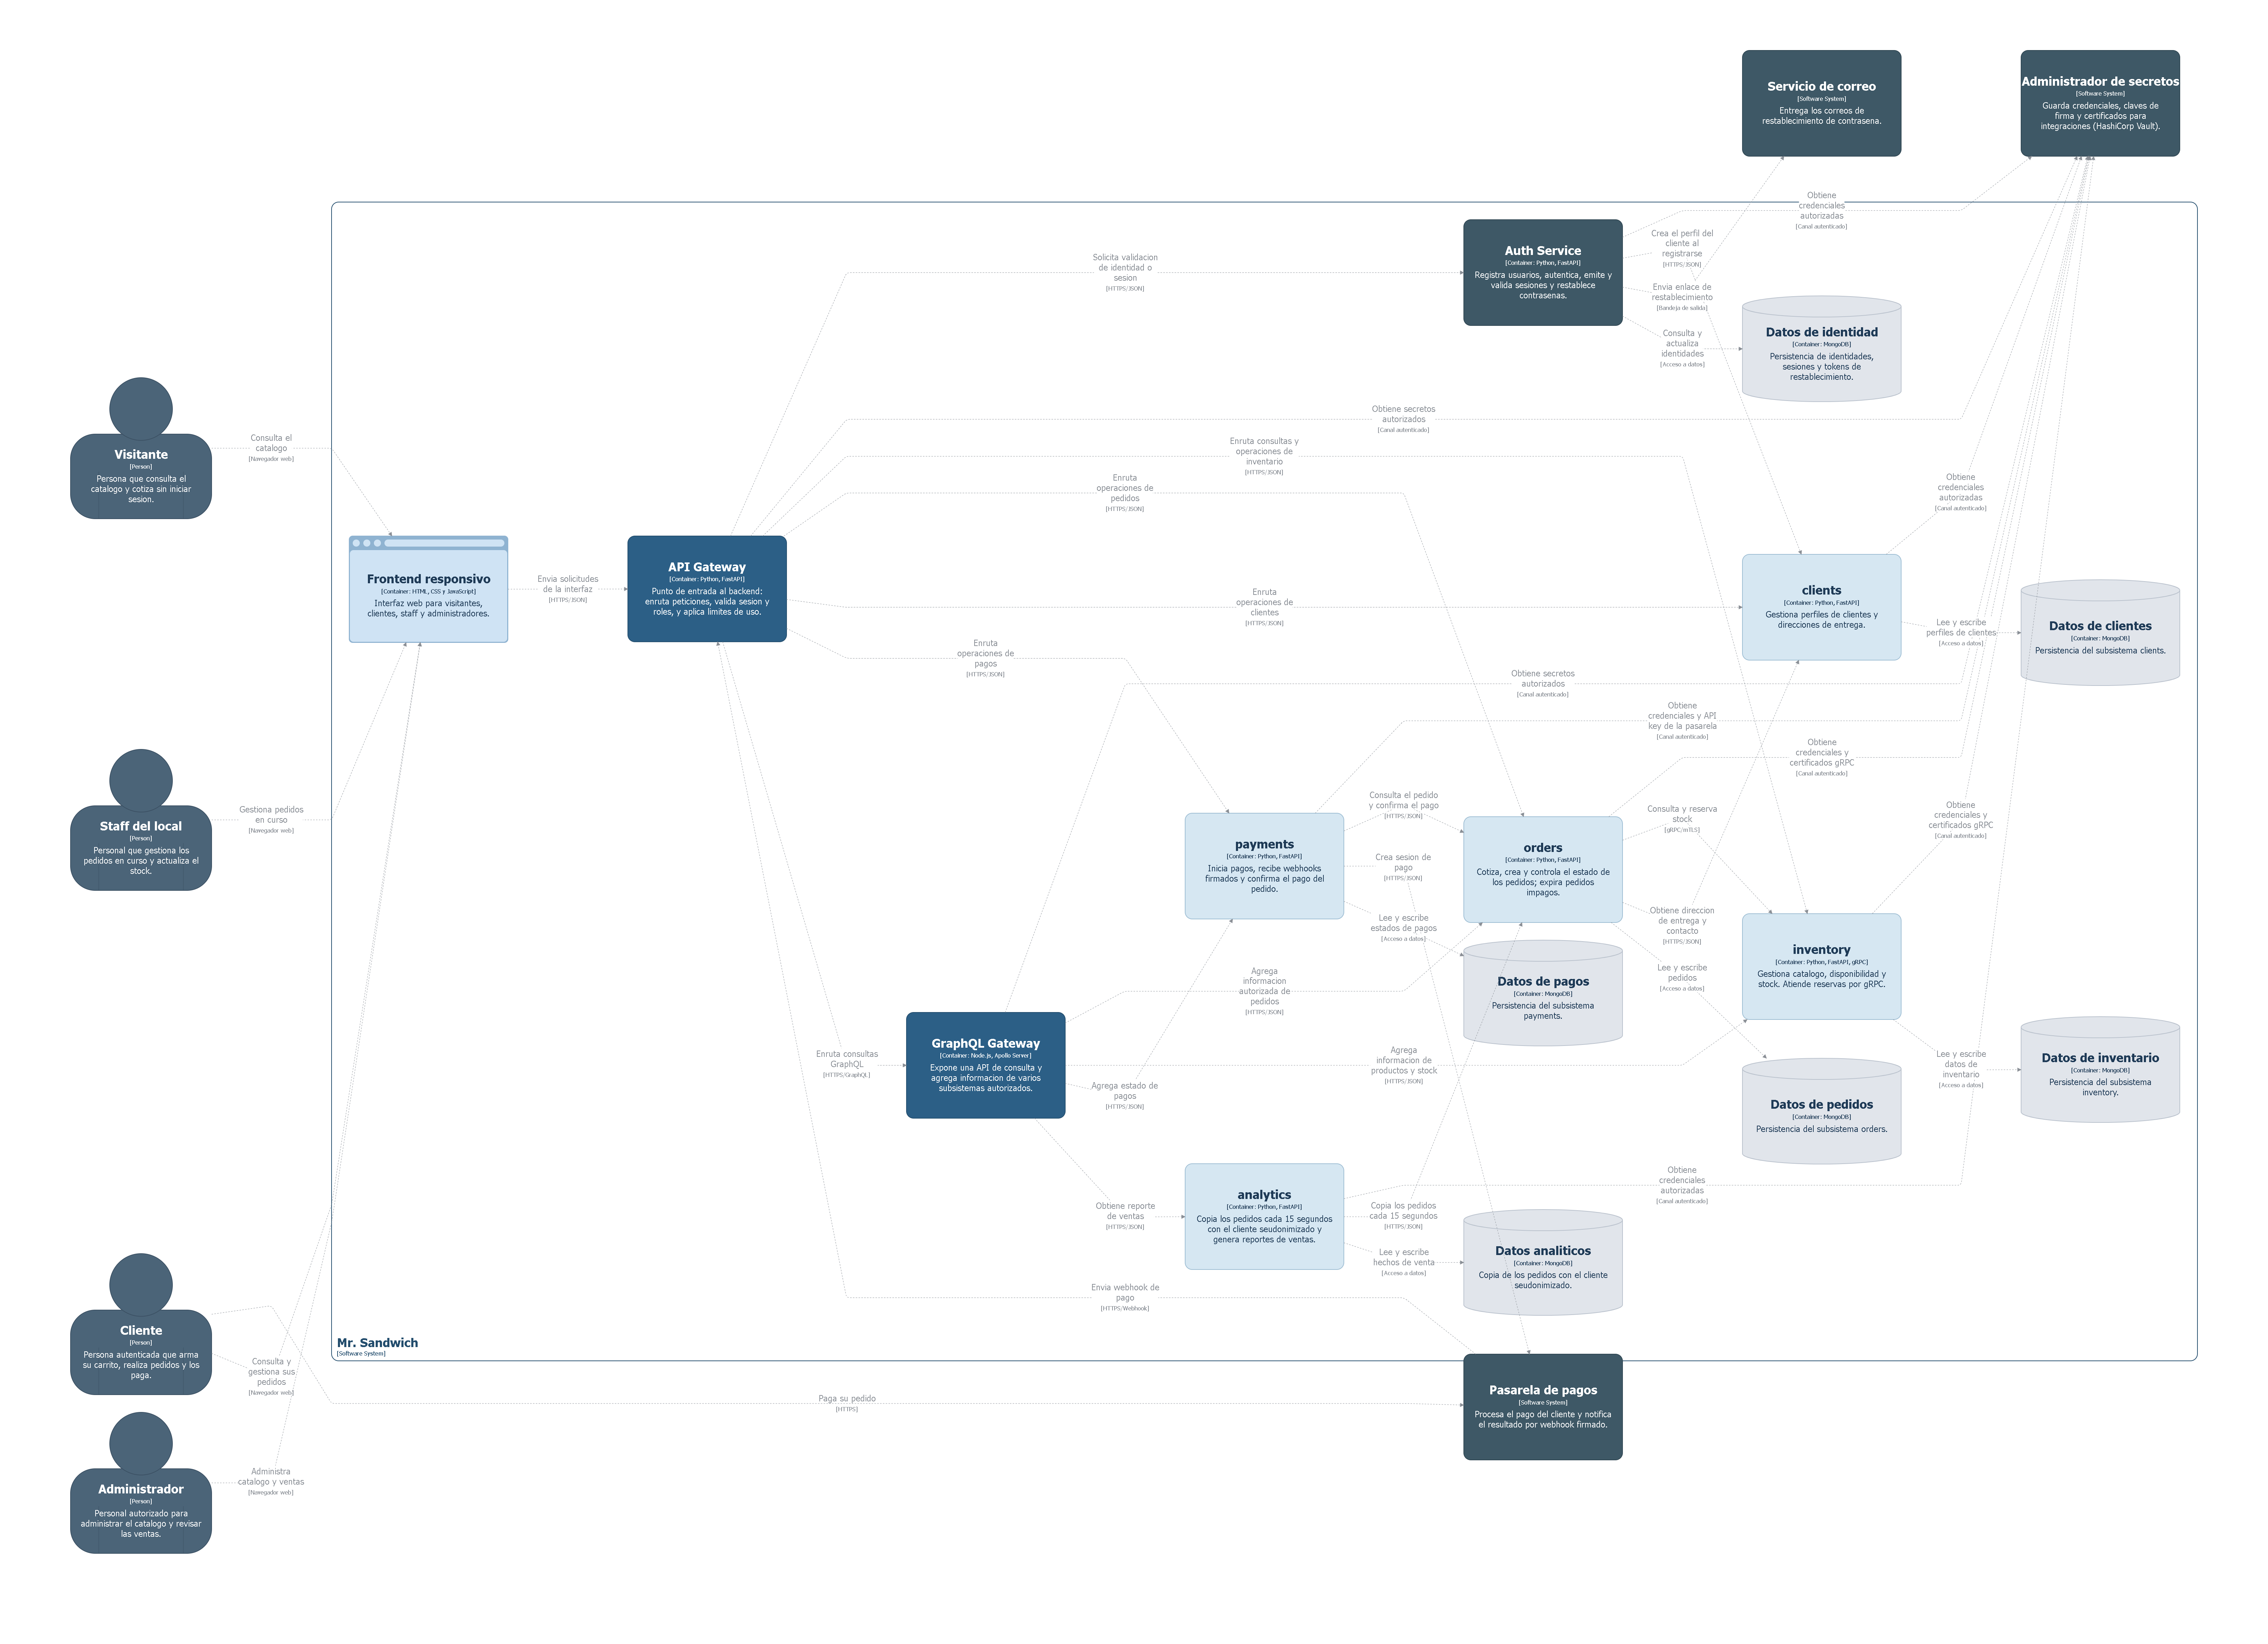
\includegraphics[width=\linewidth,height=0.78\textwidth,keepaspectratio]{c4_C2_Contenedores.png}
\caption{Mapa de componentes}
\end{figure}
\end{landscape}
\begin{figure}[H]
\centering
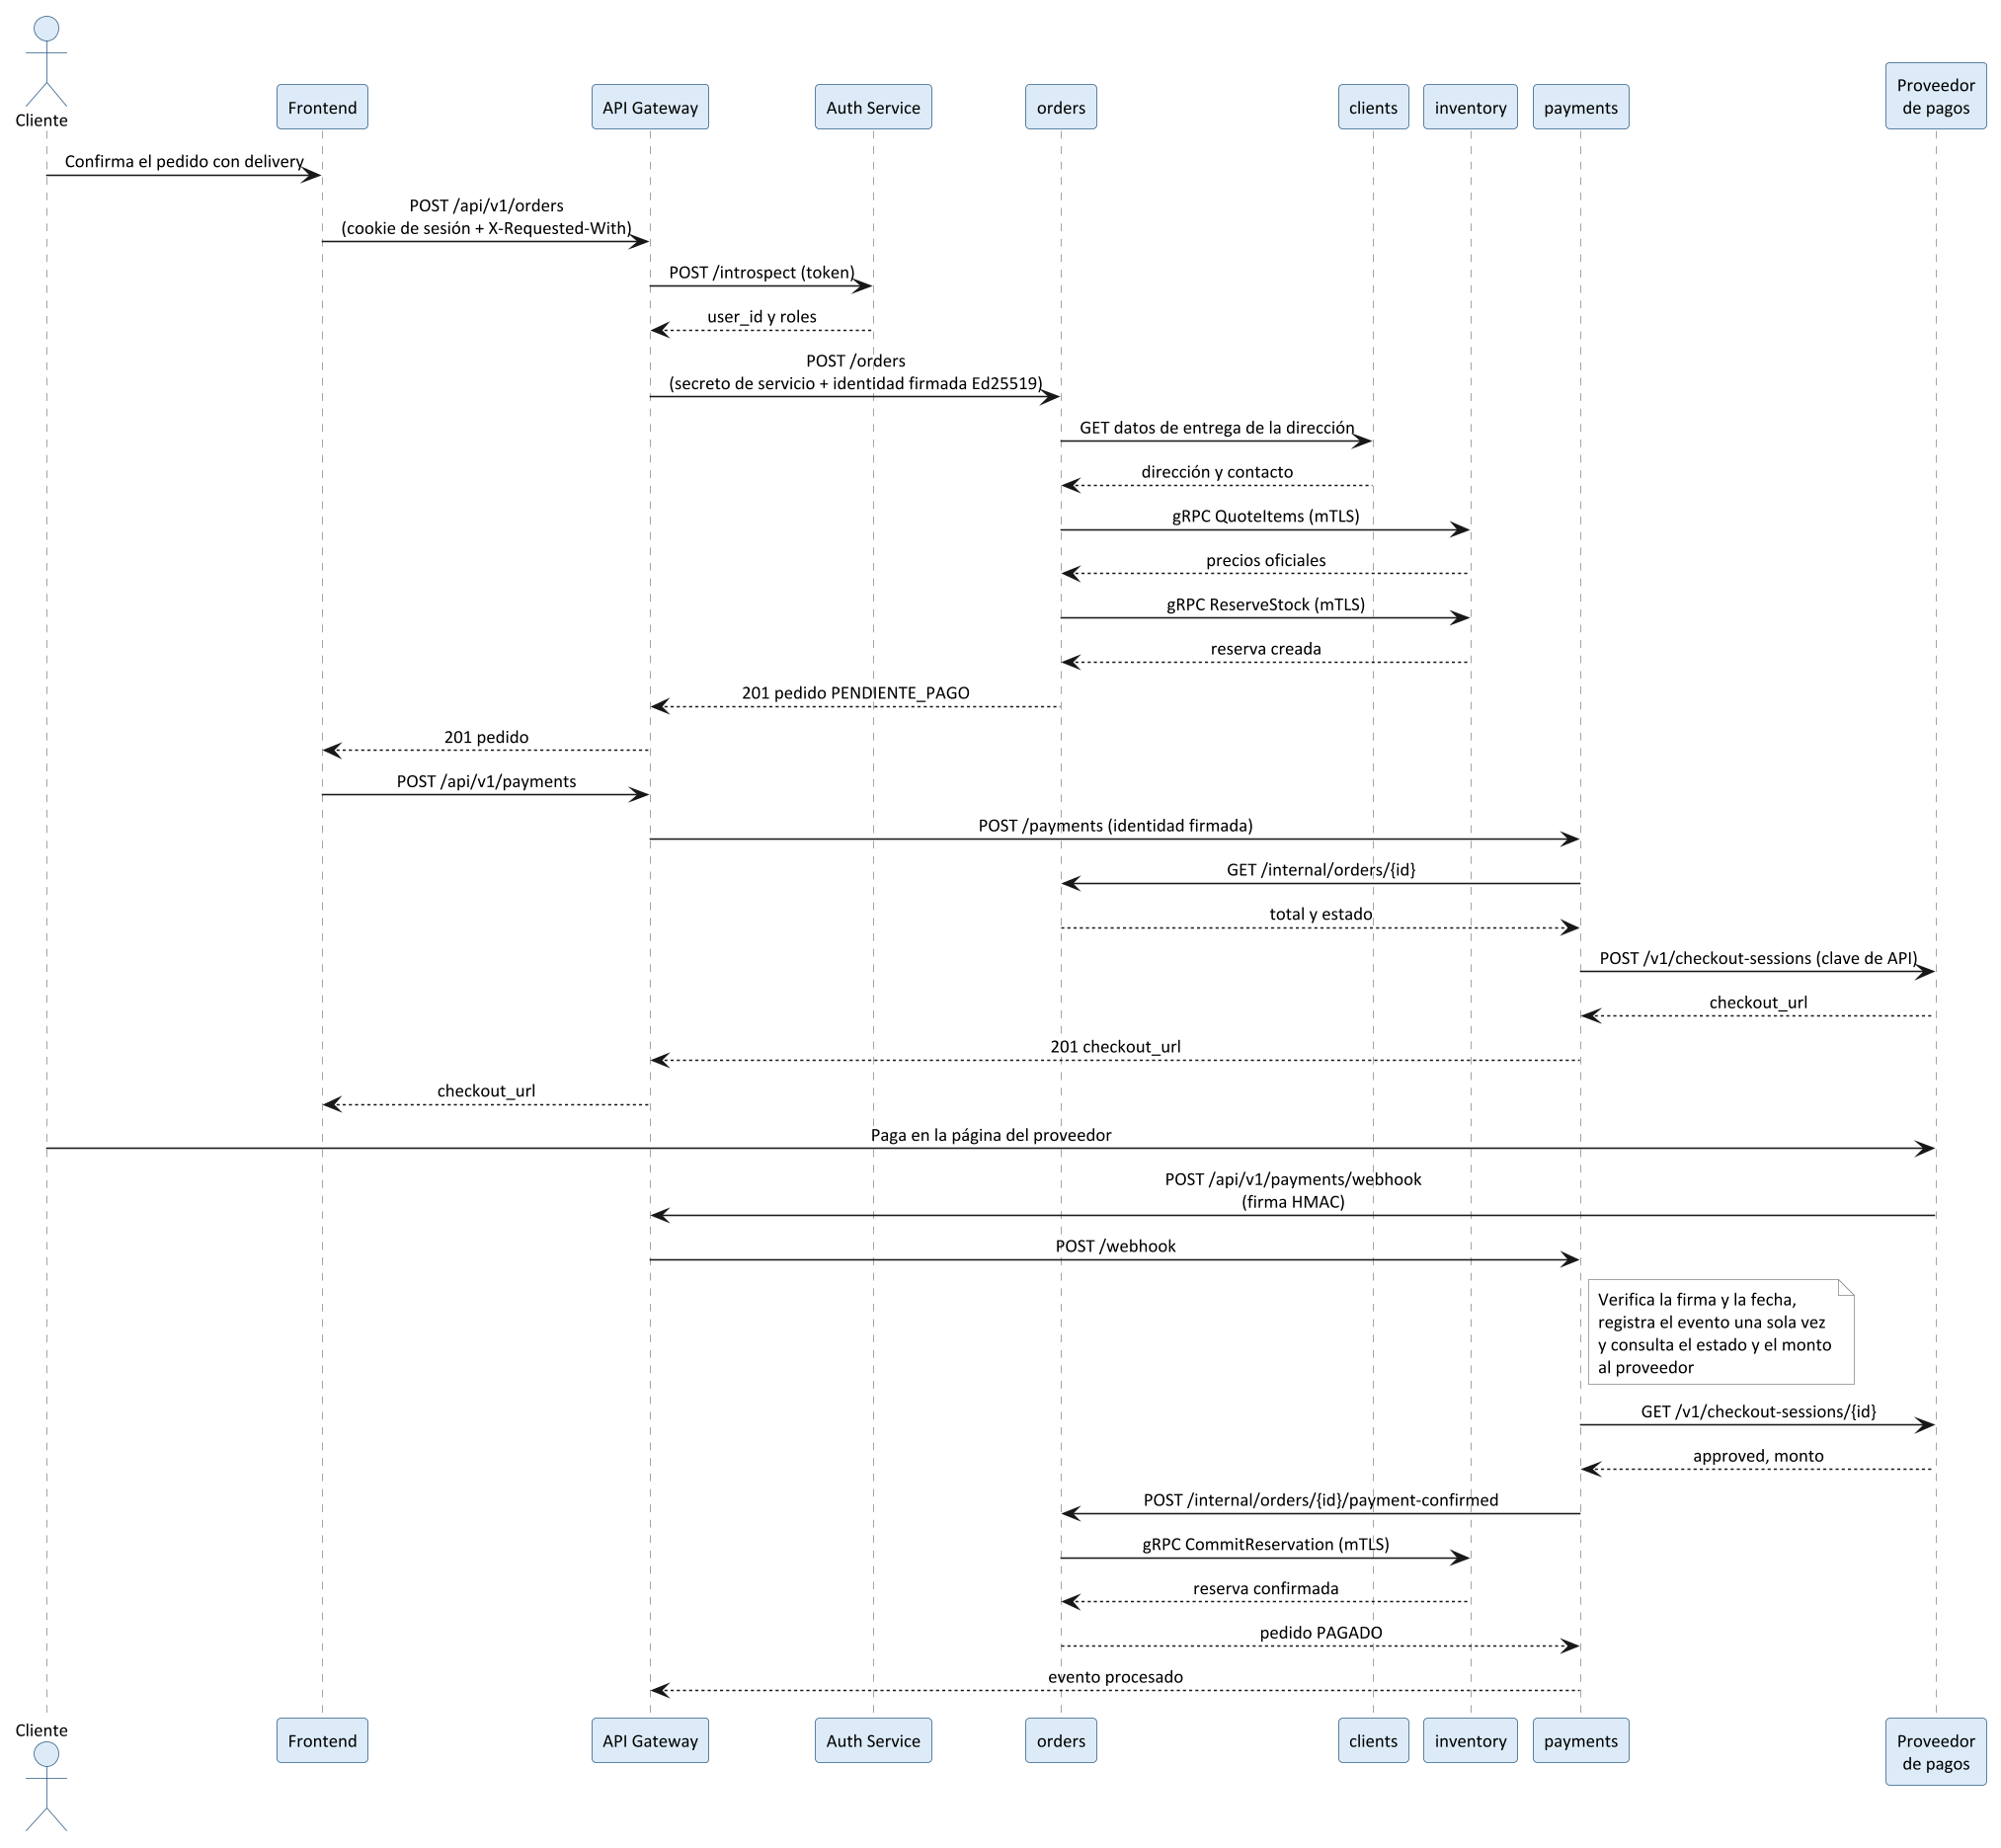
\includegraphics[width=\textwidth,height=0.8\textheight,keepaspectratio]{secuencia_compra.png}
\caption{Secuencia de compra con delivery y pago}
\end{figure}
\begin{landscape}

\subsection*{3.1 Matriz de sistemas}\phantomsection\addcontentsline{toc}{subsection}{3.1 Matriz de sistemas}
{\scriptsize
\begin{longtable}{|P{\dimexpr 0.0885\linewidth-2\tabcolsep\relax}|P{\dimexpr 0.1322\linewidth-2\tabcolsep\relax}|P{\dimexpr 0.1668\linewidth-2\tabcolsep\relax}|P{\dimexpr 0.0756\linewidth-2\tabcolsep\relax}|P{\dimexpr 0.0683\linewidth-2\tabcolsep\relax}|P{\dimexpr 0.1332\linewidth-2\tabcolsep\relax}|P{\dimexpr 0.1406\linewidth-2\tabcolsep\relax}|P{\dimexpr 0.1797\linewidth-2\tabcolsep\relax}|}
\hline
\textbf{Sistema} & \textbf{Responsabilidad} & \textbf{Datos bajo autoridad } & \textbf{Servicios} & \textbf{Dependencias} & \textbf{Contrato de integración} & \textbf{Credencial o identidad} & \textbf{Respuesta ante fallos} \\ \hline
\endfirsthead
\hline
\textbf{Sistema} & \textbf{Responsabilidad} & \textbf{Datos bajo autoridad } & \textbf{Servicios} & \textbf{Dependencias} & \textbf{Contrato de integración} & \textbf{Credencial o identidad} & \textbf{Respuesta ante fallos} \\ \hline
\endhead
\textbf{inventory} & Catálogo, precios, personalización, stock y reservas & products, categories, customization, reservations (ms\_\allowbreak{}inventory). Decide precio y stock & S01, S01b, S02, S15 (vía orders), S25–S29 & ninguno & REST (gateway, graphql), gRPC InventoryService (orders) & REST: in\_\allowbreak{}gateway, in\_\allowbreak{}graphql. gRPC certificado de la CA interna con CN=orders & Reserva atómica por producto con reversión, idempotente por order\_\allowbreak{}id \\ \hline
\textbf{orders} & Creación y ciclo de vida del pedido transiciones expiración & orders (ms\_\allowbreak{}orders). Decide el estado del pedido & S15–S21 & inventory (gRPC), clients (REST) & REST + gRPC; payment-confirmed interno & in\_\allowbreak{}gateway, in\_\allowbreak{}graphql, in\_\allowbreak{}payments, in\_\allowbreak{}analytics, out\_\allowbreak{}clients,\allowbreak{}certificado de cliente gRPC & Si inventory no responde 503 y no se guarda nada. Si falla la liberación o confirmación de stock, se marca y la tarea periódica (cada 10 s) reintenta \\ \hline
\textbf{clients} & Perfil y direcciones (datos personales) & clients, addresses (ms\_\allowbreak{}clients). Decide los datos personales & S09–S14 & ninguno & REST interno crear perfil (auth), datos de entrega (orders) & in\_\allowbreak{}gateway, in\_\allowbreak{}auth, in\_\allowbreak{}orders & Si falla durante el registro, auth compensa borrando la credencial \\ \hline
\textbf{payments} & Inicio de pagos, verificación con el proveedor, comprobantes & payments, processed\_\allowbreak{}events (ms\_\allowbreak{}payments). Decide el estado del pago y es el único que puede pedir PAGADO & S22–S24 & orders, proveedor externo & REST webhook firmado API del proveedor & in\_\allowbreak{}gateway, in\_\allowbreak{}graphql, out\_\allowbreak{}orders, provider\_\allowbreak{}api\_\allowbreak{}key, provider\_\allowbreak{}webhook\_\allowbreak{}secret & Proveedor caído el intento queda FALLIDO y se responde 503. Orders caído en el webhook se responde 503 y se borra el evento para que el proveedor reintente. Pedido ya expirado REQUIERE\_\allowbreak{}REEMBOLSO \\ \hline
\textbf{auth } & Credenciales, sesiones, recuperación & credentials, sessions, reset\_\allowbreak{}tokens (ms\_\allowbreak{}auth) & S03–S07 & clients & REST (solo gateway) & in\_\allowbreak{}gateway, out\_\allowbreak{}clients & Bloqueo tras 5 fallos; sesiones con TTL \\ \hline
\textbf{analytics (} & Reportes de ventas & order\_\allowbreak{}facts, etl\_\allowbreak{}state (ms\_\allowbreak{}analytics). Copia, no autoridad & S30 (panelAdmin.\allowbreak{}ventas) & orders & ETL GET /\allowbreak{}internal/\allowbreak{}orders-export & out\_\allowbreak{}orders, in\_\allowbreak{}graphql & Si orders cae, reintenta en el siguiente ciclo, el reporte informa actualizado\_\allowbreak{}en \\ \hline
\end{longtable}}
\end{landscape}
Como equipo decidimos separar el backend por responsabilidades, pero sin crear un servicio distinto para cada tabla. Inventory administra productos y stock, orders se encarga de los pedidos, clients gestiona los datos de clientes, y payments verifica los pagos. Esta división facilita entender quién puede modificar cada dato y evita mezclar reglas que cumplen funciones diferentes.


\subsection*{3.2 Intercambios entre sistemas}\phantomsection\addcontentsline{toc}{subsection}{3.2 Intercambios entre sistemas}
{\footnotesize
\begin{longtable}{|P{\dimexpr 0.1793\linewidth-2\tabcolsep\relax}|P{\dimexpr 0.2288\linewidth-2\tabcolsep\relax}|P{\dimexpr 0.2216\linewidth-2\tabcolsep\relax}|P{\dimexpr 0.1408\linewidth-2\tabcolsep\relax}|P{\dimexpr 0.2145\linewidth-2\tabcolsep\relax}|}
\hline
\textbf{Origen  destino} & \textbf{Operación} & \textbf{Datos mínimos} & \textbf{Autenticación} & \textbf{Errores} \\ \hline
\endfirsthead
\hline
\textbf{Origen  destino} & \textbf{Operación} & \textbf{Datos mínimos} & \textbf{Autenticación} & \textbf{Errores} \\ \hline
\endhead
orders  inventory & gRPC QuoteItems & ids, opción, extras, qty & mTLS (CN=orders) & INVALID\_\allowbreak{}ARGUMENT 400, FAILED\_\allowbreak{}PRECONDITION 409, timeout 503 \\ \hline
orders inventory & gRPC ReserveStock , ReleaseReservation , CommitReservation & order\_\allowbreak{}id, [product\_\allowbreak{}id, qty] & mTLS & RESOURCE\_\allowbreak{}EXHAUSTED 409 idempotentes \\ \hline
orders clients & GET /\allowbreak{}internal/\allowbreak{}clients/\allowbreak{}\{u\}/\allowbreak{}delivery-data/\allowbreak{}\{dir\} & dirección y contacto (nombre, teléfono) & out\_\allowbreak{}clients & 404 si la dirección no es del usuario \\ \hline
auth  clients & POST /\allowbreak{}internal/\allowbreak{}clients & user\_\allowbreak{}id, nombre, email, teléfono & out\_\allowbreak{}clients & 201 se compensa \\ \hline
payments orders & GET /\allowbreak{}internal/\allowbreak{}orders/\allowbreak{}\{id\}; POST …/\allowbreak{}payment-confirmed & id, user\_\allowbreak{}id, estado, total payment\_\allowbreak{}id & out\_\allowbreak{}orders & 409 pedido no pagable \\ \hline
analytics  orders & GET /\allowbreak{}internal/\allowbreak{}orders-export?\allowbreak{}since & sin dirección, contacto ni user\_\allowbreak{}id; cliente\_\allowbreak{}ref = HMAC & out\_\allowbreak{}orders & Reintenta en el siguiente ciclo \\ \hline
graphql orders/\allowbreak{}inventory/\allowbreak{}payments/\allowbreak{}analytics & REST con la identidad reenviada & según el campo pedido & out\_\allowbreak{}+ identidad firmada & Error parcial por campo \\ \hline
\end{longtable}}
\textbf{Control de stock:} Antes de aceptar un pedido, orders solicita a inventory que reserve las unidades necesarias. En el diseño descrito se utiliza una actualización condicional y atómica de MongoDB. Si no hay suficientes productos, se revierten las reservas anteriores, si la comunicación supera el plazo establecido de dos segundos, no se confirma el pedido, esto busca evitar ventas de unidades que ya no están disponibles.

\textbf{Confirmación del pago:} El navegador nunca informa por sí solo que una compra fue pagada. El servicio payments comprueba la firma y la fecha de la notificación, evita procesar un mismo evento dos veces y consulta el estado y el monto al proveedor. Solo después se comunica la aprobación del pago al servicio de pedidos.


\section*{Módulo 4  Stakeholders y permisos HTTP}\phantomsection\addcontentsline{toc}{section}{Módulo 4  Stakeholders y permisos HTTP}

\subsection*{4.1 Registro de stakeholders}\phantomsection\addcontentsline{toc}{subsection}{4.1 Registro de stakeholders}
{\footnotesize
\begin{longtable}{|P{\dimexpr 0.2086\linewidth-2\tabcolsep\relax}|P{\dimexpr 0.2033\linewidth-2\tabcolsep\relax}|P{\dimexpr 0.2184\linewidth-2\tabcolsep\relax}|P{\dimexpr 0.3547\linewidth-2\tabcolsep\relax}|}
\hline
\textbf{Stakeholder} & \textbf{Interés} & \textbf{Rol asociado} & \textbf{Uso de la información} \\ \hline
\endfirsthead
\hline
\textbf{Stakeholder} & \textbf{Interés} & \textbf{Rol asociado} & \textbf{Uso de la información} \\ \hline
\endhead
Visitante & Ver el menú y precios & anónimo & Catálogo público \\ \hline
Cliente registrado & Comprar, pagar, seguir pedidos & cliente & Sus propios datos, pedidos y pagos \\ \hline
Personal de cocina y despacho & Preparar y entregar a tiempo & staff & Pedidos en curso con dirección y contacto, ajuste de stock \\ \hline
Administrador del local & Catálogo, precios, ventas & admin & Todo lo anterior más productos, reportes y anulaciones con reembolso \\ \hline
Dueño /\allowbreak{} gerencia & Rentabilidad & sin permisos operativos & Recibe del administrador los reportes de ventas \\ \hline
Proveedores de insumos & Reposición & sin permisos operativos & El administrador les comunica las alertas de stock bajo por los canales habituales \\ \hline
Repartidor externo & Entregar el pedido & sin permisos operativos & Recibe del personal la dirección y el contacto del pedido asignado \\ \hline
Proveedor de pagos & Cobrar y notificar & identidad técnica provider & Solo S24, autenticado por firma HMAC \\ \hline
Microservicios internos & Colaborar & identidades técnicas gateway, auth, orders, payments, analytics, graphql & Solo las rutas internas listadas en el Módulo 6 \\ \hline
\end{longtable}}

\subsection*{4.2 Matriz de permisos}\phantomsection\addcontentsline{toc}{subsection}{4.2 Matriz de permisos}
Para interpretar los permisos: P = permitido, D = denegado, /\allowbreak{}  = no corresponde. Además indicamos qué componente realiza la verificación: G = API Gateway, M = microservicio, Q = GraphQL Gateway. Un permiso depende tanto del rol como del pedido o recurso al que se quiere acceder.

{\scriptsize
\begin{longtable}{|P{\dimexpr 0.1193\linewidth-2\tabcolsep\relax}|P{\dimexpr 0.1560\linewidth-2\tabcolsep\relax}|P{\dimexpr 0.1727\linewidth-2\tabcolsep\relax}|P{\dimexpr 0.0990\linewidth-2\tabcolsep\relax}|P{\dimexpr 0.0965\linewidth-2\tabcolsep\relax}|P{\dimexpr 0.2447\linewidth-2\tabcolsep\relax}|P{\dimexpr 0.0968\linewidth-2\tabcolsep\relax}|}
\hline
\textbf{Rol /\allowbreak{} identidad} & \textbf{Servicio} & \textbf{Ruta} & \textbf{Verbo} & \textbf{Decisión} & \textbf{Alcance y condición} & \textbf{Dónde} \\ \hline
\endfirsthead
\hline
\textbf{Rol /\allowbreak{} identidad} & \textbf{Servicio} & \textbf{Ruta} & \textbf{Verbo} & \textbf{Decisión} & \textbf{Alcance y condición} & \textbf{Dónde} \\ \hline
\endhead
Visitante & S01, S01b, S02, S15 & /\allowbreak{}products…, /\allowbreak{}categories, /\allowbreak{}orders/\allowbreak{}quote & GET y POST & P & Solo campos públicos & G \\ \hline
Visitante & S03, S04, S06, S07 & /\allowbreak{}auth/\allowbreak{}… & POST & P & Límite de 20 por minuto e IP & G \\ \hline
Cliente & S09–S14 & /\allowbreak{}clients/\allowbreak{}me… & GET/\allowbreak{}PUT/\allowbreak{}POST/\allowbreak{}DELETE & P & Solo los propios: el user\_\allowbreak{}id sale de la identidad firmada, nunca de la URL & M (clients) \\ \hline
Cliente & S16 & /\allowbreak{}orders & POST & P & Dirección propia, máximo 3 pedidos pendientes & G+M \\ \hline
Cliente & S17, S18 & /\allowbreak{}orders/\allowbreak{}me, /\allowbreak{}orders/\allowbreak{}\{id\} & GET & P & Solo pedidos propios, un pedido ajeno da 404 & M (orders) \\ \hline
Cliente & S19 & /\allowbreak{}orders/\allowbreak{}\{id\}/\allowbreak{}cancel & POST & P & Propio y en pendiente pago & M \\ \hline
Cliente & S21 & /\allowbreak{}orders/\allowbreak{}\{id\}/\allowbreak{}status & PUT & D (403) & /\allowbreak{} & G \\ \hline
Cliente & S22, S23 & /\allowbreak{}payments… & POST/\allowbreak{}GET & P & Pedido propio y en pendiente pago & M (payments) \\ \hline
Cliente & S25–S29 & /\allowbreak{}admin/\allowbreak{}products… & Todos & D (403) & Ver el catálogo no da permisos de administración & G+M \\ \hline
Cliente & S30 & /\allowbreak{}graphql & POST & P & resumenPedido y misPedidos propios, contacto nulo, pedidosLocal y panelAdmin denegados & Q+M \\ \hline
Staff & S18, S20, S21, S23 & pedidos y pagos & GET/\allowbreak{}PUT & P & Todos los pedidos, transiciones válidas según el tipo de entrega & G+M \\ \hline
Staff & S16, S19, S22 & crear, anular, pagar & POST & D (403) & El personal no compra ni anula & G/\allowbreak{}M \\ \hline
Staff & S25, S29 & /\allowbreak{}admin/\allowbreak{}products, /\allowbreak{}admin/\allowbreak{}products/\allowbreak{}\{id\}/\allowbreak{}stock & GET/\allowbreak{}PUT & P & Ver productos y ajustar stock & G+M \\ \hline
Staff & S26–S28 & crear, editar, dar de baja productos & POST/\allowbreak{}PUT/\allowbreak{}DELETE & D (403) & /\allowbreak{} & G+M \\ \hline
Admin & S19 & /\allowbreak{}orders/\allowbreak{}\{id\}/\allowbreak{}cancel & POST & P & Pendiente o pagado & M \\ \hline
Admin & S25–S29, S30 panelAdmin & administración y reportes & Todos & P & /\allowbreak{} & G+M+Q \\ \hline
Cualquiera & marcar PAGADO & /\allowbreak{}orders/\allowbreak{}\{id\}/\allowbreak{}status & PUT & D & Solo payments, por /\allowbreak{}internal/\allowbreak{}…/\allowbreak{}payment-confirmed & M \\ \hline
Proveedor & S24 & /\allowbreak{}payments/\allowbreak{}webhook & POST & P & Firma HMAC válida y reciente & M (payments) \\ \hline
gateway & todas las internas publicadas & /\allowbreak{} & /\allowbreak{} & P & Secreto por destino + identidad firmada & M \\ \hline
orders & inventory gRPC & 4 métodos & /\allowbreak{} & P & CN=orders & M (inventory) \\ \hline
payments & orders payment-confirmed, GET /\allowbreak{}internal/\allowbreak{}orders/\allowbreak{}\{id\} & /\allowbreak{} & GET/\allowbreak{}POST & P & /\allowbreak{} & M \\ \hline
analytics & orders orders-export & /\allowbreak{} & GET & P & Datos seudonimizados & M \\ \hline
\end{longtable}}

\section*{Módulo 5  Clases del API Gateway}\phantomsection\addcontentsline{toc}{section}{Módulo 5  Clases del API Gateway}
Dibujamos un segundo diagrama UML para explicar la organización del API Gateway y sus políticas.

\begin{landscape}
\begin{figure}[H]
\centering
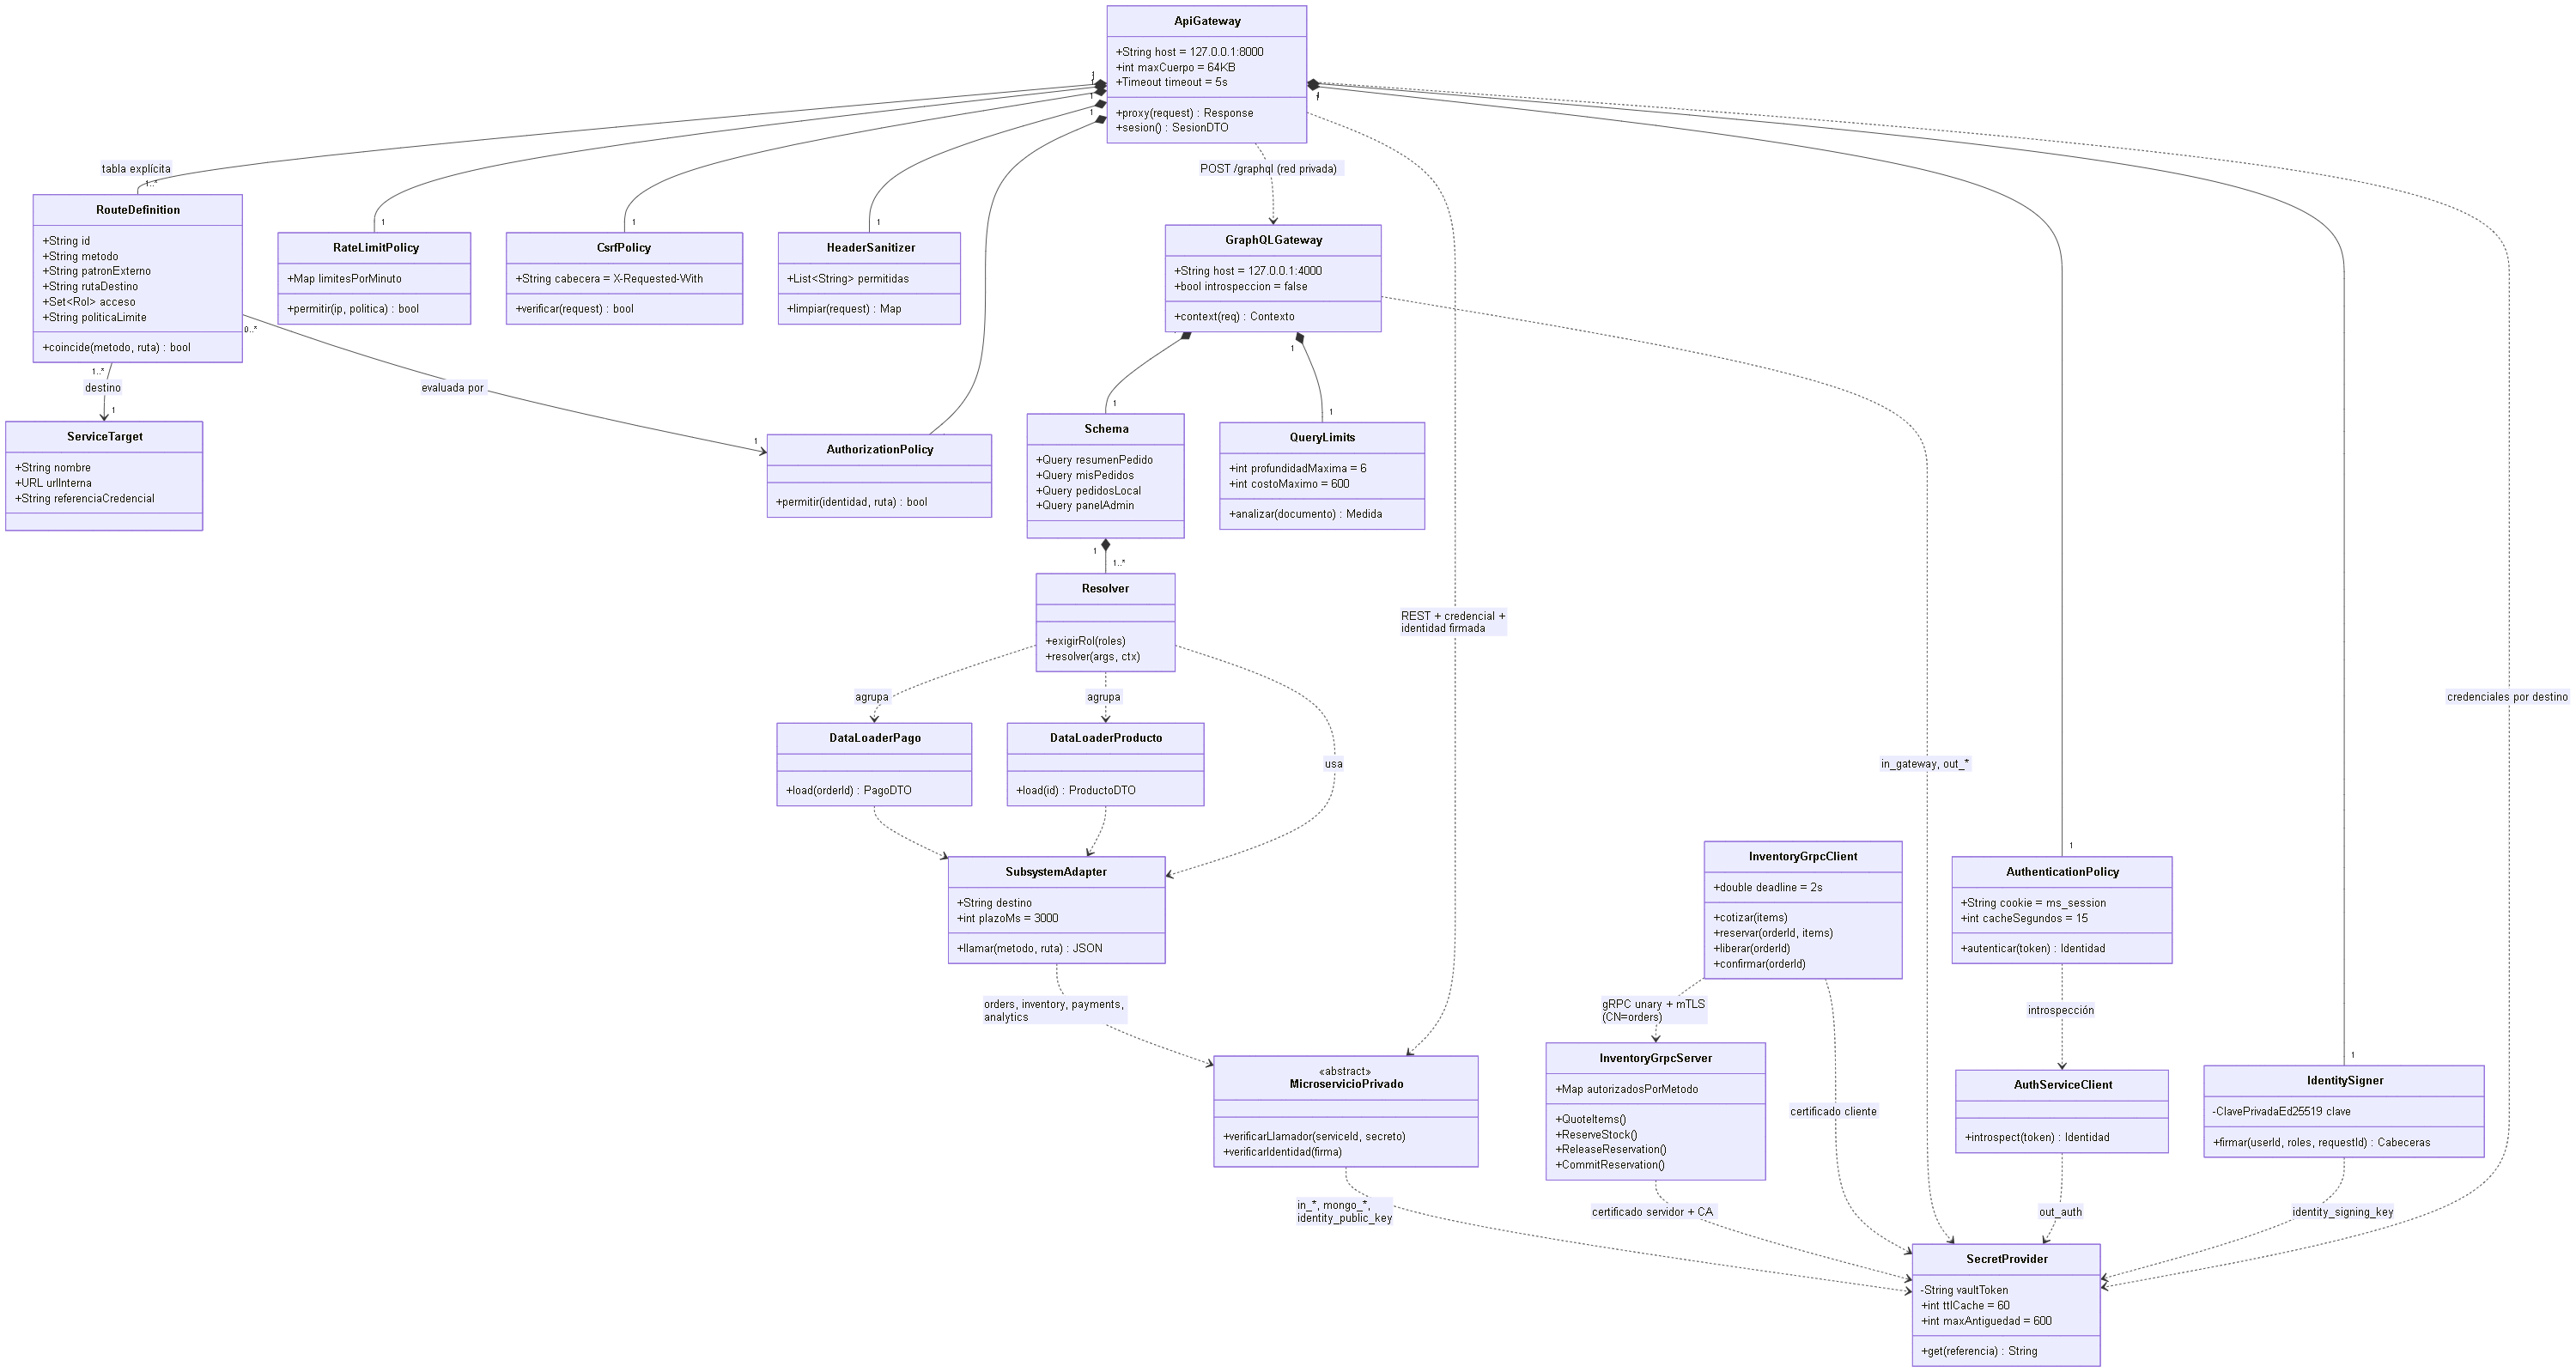
\includegraphics[width=\linewidth,height=0.78\textwidth,keepaspectratio]{uml_gateway.png}
\caption{Diagrama UML de clases del API Gateway, políticas, GraphQL Gateway y gRPC}
\end{figure}
\end{landscape}
Elegimos un API Gateway porque el frontend necesita un punto de entrada claro. En lugar de que el navegador conozca las direcciones de todos los servicios privados, envía las solicitudes a este componente. El Gateway decide a qué servicio dirigir cada ruta y aplica controles distintos según corresponda a una consulta pública, a un cliente o a un administrador.

Agrupamos las rutas según su acceso. Entre las públicas están el catálogo, el registro y el inicio de sesión. Las rutas de cuenta y pedidos necesitan una sesión válida, las administrativas exigen el rol adecuado. Las rutas internas, como /\allowbreak{}internal/\allowbreak{}*, /\allowbreak{}introspect o /\allowbreak{}report, no deben quedar expuestas directamente al navegador.

Para comprender la seguridad, identificamos las siguientes fronteras entre componentes:

\begin{enumerate}
\item Del navegador al Gateway no se confía automáticamente en lo recibido, se comprueban la sesión y los permisos, se limita el tamaño de la solicitud, se controlan los orígenes y se descartan las cabeceras que no deben venir del cliente.
\item Del Gateway a cada microservicio se usa una credencial propia y una identidad firmada. Con esto los servicios internos pueden verificar quién solicita la operación sin confiar en que el navegador haya escrito correctamente su identidad.
\item Entre orders e inventory se utiliza gRPC con mTLS, de forma que ambos componentes identifican al otro mediante certificados.
\item Cada microservicio usa su propia cuenta de base de datos, con permisos sobre los datos que necesita y no sobre las bases de los demás.
\end{enumerate}
El Gateway hace una primera comprobación de sesión, rol y límites. Sin embargo, cada servicio vuelve a validar la operación, porque allí se conocen las reglas del negocio. 

\textbf{Ejemplo permitido:} Cuando Ana consulta un pedido suyo, el Gateway comprueba que inició sesión y envía al servicio orders su identidad verificada. Luego orders compara al usuario con el dueño del pedido. Si coincide, responde con los datos que puede ver.

\textbf{Ejemplo rechazado:} Si Pedro intenta abrir un pedido de Ana, aunque haya iniciado sesión, orders no le permite acceder. Del mismo modo, un cliente que intenta crear productos desde una ruta de administración recibe una respuesta de acceso denegado.


\section*{Módulo 6 Rutas y secretos de integración}\phantomsection\addcontentsline{toc}{section}{Módulo 6 Rutas y secretos de integración}

\subsection*{6.1 Matriz de rutas }\phantomsection\addcontentsline{toc}{subsection}{6.1 Matriz de rutas }
En esta tabla seguimos cada solicitud desde la ruta pública hasta el servicio encargado de atenderla. Todos los accesos externos pasan por el Gateway del proyecto. La cookie del usuario se convierte en una identidad interna verificada y cada comunicación utiliza la credencial que le corresponde.

{\scriptsize
\begin{longtable}{|P{\dimexpr 0.0855\linewidth-2\tabcolsep\relax}|P{\dimexpr 0.0855\linewidth-2\tabcolsep\relax}|P{\dimexpr 0.1899\linewidth-2\tabcolsep\relax}|P{\dimexpr 0.1224\linewidth-2\tabcolsep\relax}|P{\dimexpr 0.1877\linewidth-2\tabcolsep\relax}|P{\dimexpr 0.1614\linewidth-2\tabcolsep\relax}|P{\dimexpr 0.1524\linewidth-2\tabcolsep\relax}|}
\hline
\textbf{ID} & \textbf{Verbo} & \textbf{Ruta externa} & \textbf{Acceso y rol} & \textbf{Sistema y ruta destino} & \textbf{Controles} & \textbf{Ref. credencial} \\ \hline
\endfirsthead
\hline
\textbf{ID} & \textbf{Verbo} & \textbf{Ruta externa} & \textbf{Acceso y rol} & \textbf{Sistema y ruta destino} & \textbf{Controles} & \textbf{Ref. credencial} \\ \hline
\endhead
S01 & GET & /\allowbreak{}api/\allowbreak{}v1/\allowbreak{}products & anónimo & inventory GET /\allowbreak{}products & Validación de filtros, 300/\allowbreak{}min & Gateway a inventory \\ \hline
S01b & GET & /\allowbreak{}api/\allowbreak{}v1/\allowbreak{}categories & anónimo & inventory GET /\allowbreak{}categories & 300/\allowbreak{}min & Gateway a inventory \\ \hline
S02 & GET & /\allowbreak{}api/\allowbreak{}v1/\allowbreak{}products/\allowbreak{}\{id\} & anónimo & inventory GET /\allowbreak{}products/\allowbreak{}\{id\} & Patrón de parámetro & Gateway a inventory \\ \hline
S03 & POST & /\allowbreak{}api/\allowbreak{}v1/\allowbreak{}auth/\allowbreak{}register & anónimo & auth POST /\allowbreak{}register & 20/\allowbreak{}min, 64 KB & Gateway a auth \\ \hline
S04 & POST & /\allowbreak{}api/\allowbreak{}v1/\allowbreak{}auth/\allowbreak{}login & anónimo & auth POST /\allowbreak{}login & 20/\allowbreak{}min, emite la cookie & Gateway a auth \\ \hline
S05 & POST & /\allowbreak{}api/\allowbreak{}v1/\allowbreak{}auth/\allowbreak{}logout & autenticado & auth POST /\allowbreak{}logout (token en el cuerpo) & CSRF, invalida la caché & Gateway a auth \\ \hline
S06/\allowbreak{}S07 & POST & /\allowbreak{}api/\allowbreak{}v1/\allowbreak{}auth/\allowbreak{}password-reset/\allowbreak{}* & anónimo & auth /\allowbreak{}password-reset/\allowbreak{}* & 20/\allowbreak{}min & Gateway a auth \\ \hline
S09–S14 & GET/\allowbreak{}PUT/\allowbreak{}POST/\allowbreak{}DELETE & /\allowbreak{}api/\allowbreak{}v1/\allowbreak{}clients/\allowbreak{}me[/\allowbreak{}addresses[/\allowbreak{}\{id\}]] & autenticado & clients /\allowbreak{}me… & CSRF, identidad firmada & Gateway a clients \\ \hline
S15 & POST & /\allowbreak{}api/\allowbreak{}v1/\allowbreak{}orders/\allowbreak{}quote & anónimo & orders POST /\allowbreak{}quote & 300/\allowbreak{}min & Gateway a orders \\ \hline
S16 & POST & /\allowbreak{}api/\allowbreak{}v1/\allowbreak{}orders & cliente & orders POST /\allowbreak{}orders & CSRF, Idempotency-Key validada & Gateway a orders \\ \hline
S17/\allowbreak{}S18 & GET & /\allowbreak{}api/\allowbreak{}v1/\allowbreak{}orders/\allowbreak{}me, /\allowbreak{}api/\allowbreak{}v1/\allowbreak{}orders/\allowbreak{}\{id\} & autenticado & orders /\allowbreak{}orders/\allowbreak{}me, /\allowbreak{}orders/\allowbreak{}\{id\} & Propiedad en orders & Gateway a orders \\ \hline
S19 & POST & /\allowbreak{}api/\allowbreak{}v1/\allowbreak{}orders/\allowbreak{}\{id\}/\allowbreak{}cancel & autenticado & orders /\allowbreak{}orders/\allowbreak{}\{id\}/\allowbreak{}cancel & CSRF & Gateway a orders \\ \hline
S20/\allowbreak{}S21 & GET/\allowbreak{}PUT & /\allowbreak{}api/\allowbreak{}v1/\allowbreak{}orders, /\allowbreak{}api/\allowbreak{}v1/\allowbreak{}orders/\allowbreak{}\{id\}/\allowbreak{}status & staff, admin & orders /\allowbreak{}orders, /\allowbreak{}orders/\allowbreak{}\{id\}/\allowbreak{}status & Rol en G y M & Gateway a orders \\ \hline
S22/\allowbreak{}S23 & POST/\allowbreak{}GET & /\allowbreak{}api/\allowbreak{}v1/\allowbreak{}payments, /\allowbreak{}api/\allowbreak{}v1/\allowbreak{}payments/\allowbreak{}order/\allowbreak{}\{id\} & cliente /\allowbreak{} autenticado & payments /\allowbreak{}payments… & CSRF; propiedad & Gateway a payments \\ \hline
S24 & POST & /\allowbreak{}api/\allowbreak{}v1/\allowbreak{}payments/\allowbreak{}webhook & proveedor & payments POST /\allowbreak{}webhook & 120/\allowbreak{}min; firma HMAC en payments, sin CSRF & Gateway a payments \\ \hline
S25–S29 & GET & /\allowbreak{}api/\allowbreak{}v1/\allowbreak{}admin/\allowbreak{}products… & staff /\allowbreak{} admin & inventory /\allowbreak{}admin/\allowbreak{}products… & Rol en G y M & Gateway a nventory \\ \hline
S30 & POST & /\allowbreak{}api/\allowbreak{}v1/\allowbreak{}graphql & autenticado & graphql POST /\allowbreak{}graphql & 120/\allowbreak{}mi, costo y profundidad en Q & Gateway a graphql \\ \hline
S31 & GET & /\allowbreak{}api/\allowbreak{}v1/\allowbreak{}session & cualquiera & local en el gateway & /\allowbreak{} & Gateway a auth  \\ \hline
\end{longtable}}

\subsection*{6.2 Operaciones GraphQL}\phantomsection\addcontentsline{toc}{subsection}{6.2 Operaciones GraphQL}
{\footnotesize
\begin{longtable}{|P{\dimexpr 0.1481\linewidth-2\tabcolsep\relax}|P{\dimexpr 0.0710\linewidth-2\tabcolsep\relax}|P{\dimexpr 0.2733\linewidth-2\tabcolsep\relax}|P{\dimexpr 0.2299\linewidth-2\tabcolsep\relax}|P{\dimexpr 0.2628\linewidth-2\tabcolsep\relax}|}
\hline
\textbf{Operación} & \textbf{Tipo} & \textbf{Campos autorizados} & \textbf{Resolver} & \textbf{Subsistemas} \\ \hline
\endfirsthead
\hline
\textbf{Operación} & \textbf{Tipo} & \textbf{Campos autorizados} & \textbf{Resolver} & \textbf{Subsistemas} \\ \hline
\endhead
resumenPedido & Query & Todos para el dueño excepto contacto, staff y admin, todos & Query.\allowbreak{}resumenPedido, ResumenPedido.\allowbreak{}pago, LineaPedido.\allowbreak{}producto, ResumenPedido.\allowbreak{}contacto & orders, inventory (lote), payments (lote) \\ \hline
misPedidos & Query & Igual que arriba, solo pedidos propios & Query.\allowbreak{}misPedidos + DataLoaders & orders, inventory, payments \\ \hline
pedidosLocal & Query & Staff y admin (incluye contacto y direccionEntrega) & Query.\allowbreak{}pedidosLocal & orders, inventory, payments \\ \hline
panelAdmin( & Query & Solo admin & PanelAdmin.\allowbreak{}ventas, PanelAdmin.\allowbreak{}stockBajo & analytics, inventory \\ \hline
\end{longtable}}

\subsection*{6.3 Métodos gRPC }\phantomsection\addcontentsline{toc}{subsection}{6.3 Métodos gRPC }
{\footnotesize
\begin{longtable}{|P{\dimexpr 0.1825\linewidth-2\tabcolsep\relax}|P{\dimexpr 0.1901\linewidth-2\tabcolsep\relax}|P{\dimexpr 0.0831\linewidth-2\tabcolsep\relax}|P{\dimexpr 0.1808\linewidth-2\tabcolsep\relax}|P{\dimexpr 0.0961\linewidth-2\tabcolsep\relax}|P{\dimexpr 0.2524\linewidth-2\tabcolsep\relax}|}
\hline
\textbf{Servicio.\allowbreak{}método} & \textbf{Entrada y salida} & \textbf{Modalidad} & \textbf{Identidad permitida} & \textbf{Plazo máximo} & \textbf{Idempotencia} \\ \hline
\endfirsthead
\hline
\textbf{Servicio.\allowbreak{}método} & \textbf{Entrada y salida} & \textbf{Modalidad} & \textbf{Identidad permitida} & \textbf{Plazo máximo} & \textbf{Idempotencia} \\ \hline
\endhead
InventoryService.\allowbreak{}QuoteItems & QuoteRequest y QuoteResponse & unary & CN=orders & 2 s & Lectura \\ \hline
InventoryService.\allowbreak{}ReserveStock & ReserveRequest y ReservationResponse & unary & CN=orders & 2 s & Por order\_\allowbreak{}id \\ \hline
InventoryService.\allowbreak{}ReleaseReservation & ReservationRef y ReservationResponse & unary & CN=orders & 2 s & Sí \\ \hline
InventoryService.\allowbreak{}CommitReservation & ReservationRef y ReservationResponse & unary & CN=orders & 2 s & Sí \\ \hline
\end{longtable}}
En el contrato gRPC se establecieron límites de tamaño de mensajes y de cantidad de ítems, además de un número de hilos de atención. El objetivo es evitar solicitudes excesivas que puedan afectar al servicio de inventario.

\begin{landscape}

\subsection*{6.4 Inventario simbólico de secretos e identidades}\phantomsection\addcontentsline{toc}{subsection}{6.4 Inventario simbólico de secretos e identidades}
En este apartado registramos los secretos necesarios para que los servicios se comuniquen. Todos los secretos se generan en scripts/\allowbreak{}bootstrap.\allowbreak{}py y se guardan en Vault siendo secret/\allowbreak{}mrsandwich/\allowbreak{}consumidor. Cada consumidor recibe un token de Vault propio cuya política solo permite leer su ruta.\allowbreak{}Cada componente debería acceder solo a la credencial que necesita para cumplir su función.

{\scriptsize
\begin{longtable}{|P{\dimexpr 0.1467\linewidth-2\tabcolsep\relax}|P{\dimexpr 0.1145\linewidth-2\tabcolsep\relax}|P{\dimexpr 0.0951\linewidth-2\tabcolsep\relax}|P{\dimexpr 0.1118\linewidth-2\tabcolsep\relax}|P{\dimexpr 0.1382\linewidth-2\tabcolsep\relax}|P{\dimexpr 0.1051\linewidth-2\tabcolsep\relax}|P{\dimexpr 0.1033\linewidth-2\tabcolsep\relax}|P{\dimexpr 0.1704\linewidth-2\tabcolsep\relax}|}
\hline
\textbf{Referencia} & \textbf{Tipo} & \textbf{Emisor} & \textbf{Consumidor} & \textbf{Finalidad} & \textbf{Ubicación} & \textbf{Alcance} & \textbf{Rotación /\allowbreak{} revocación} \\ \hline
\endfirsthead
\hline
\textbf{Referencia} & \textbf{Tipo} & \textbf{Emisor} & \textbf{Consumidor} & \textbf{Finalidad} & \textbf{Ubicación} & \textbf{Alcance} & \textbf{Rotación /\allowbreak{} revocación} \\ \hline
\endhead
Gateway \{auth,\allowbreak{}clients,\allowbreak{}inventory,\allowbreak{}orders,\allowbreak{}payments,\allowbreak{}graphql\} & Secreto compartido por par  & bootstrap & gateway (out\_\allowbreak{}*) /\allowbreak{} destino (in\_\allowbreak{}gateway) & Autenticar al gateway ante cada servicio & Vault & Un par = un destino & Nuevo en cada arranque, revocar = reiniciar o reescribir solo ese par \\ \hline
Auth a clients, orders a clients, payments a orders, analytics a orders, graphql a \{orders,\allowbreak{}inventory,\allowbreak{}payments,\allowbreak{}analytics\} & Secreto por par & bootstrap & llamador /\allowbreak{} destino & Llamadas internas & Vault & Solo las rutas internas de ese par & Cada arranque \\ \hline
identity\_\allowbreak{}signing\_\allowbreak{}key & Clave privada Ed25519 & bootstrap & solo gateway & Firmar el contexto de identidad & Vault & Firmar & Cada arranque invalida firmas anteriores, su vigencia es de 60 s \\ \hline
identity\_\allowbreak{}public\_\allowbreak{}key & Clave pública & bootstrap & servicios y graphql & Verificar identidad & Vault & Verificar & Junto con la privada \\ \hline
grpc\_\allowbreak{}ca\_\allowbreak{}cert + grpc\_\allowbreak{}server\_\allowbreak{}* /\allowbreak{} grpc\_\allowbreak{}client\_\allowbreak{}* & CA interna EC P-256 + certificados (1 día) & bootstrap & inventory (servidor), orders (cliente) & mTLS gRPC & Vault & CN = identidad & Cada arranque, el certificado vence en 24 h \\ \hline
mongo\_\allowbreak{}user /\allowbreak{} mongo\_\allowbreak{}password por servicio & Credencial de base de datos & bootstrap con el admin de Mongo & Solo su servicio & Acceso a su base  & Vault & Una base & La contraseña rota en cada arranque \\ \hline
Admin de MongoDB & Credencial root & bootstrap en primer arranque & Solo bootstrap, seed y run\_\allowbreak{}all stop & Crear y rotar usuarios & \textasciitilde{}/\allowbreak{}.mrsandwich/\allowbreak{}runtime/\allowbreak{}mongo-admin.\allowbreak{}json fuera de OneDrive y del repo & root & Manual: cambiarla con db.\allowbreak{}changeUserPassword y actualizar el archivo \\ \hline
provider\_\allowbreak{}api\_\allowbreak{}key & API key del comercio & Proveedor de pagos & payments & Crear y consultar sesiones de pago & Vault & Solo la API del comercio, nunca llega al navegador & La emite el proveedor \\ \hline
provider\_\allowbreak{}webhook\_\allowbreak{}secret & Secreto HMAC & Proveedor de pagos & payments & Verificar notificaciones & Vault & Solo verificar & Como la API key \\ \hline
analytics\_\allowbreak{}pseudonym\_\allowbreak{}key & Clave HMAC & bootstrap & orders & Seudonimizar al cliente en la analítica & Archivo en runtime a Vault & Seudónimos & Estable rotación anual junto con el reinicio de ms\_\allowbreak{}analytics \\ \hline
Token raíz de Vault & Token de administración & run\_\allowbreak{}all & Solo bootstrap & Configurar Vault & Memoria, no se escribe, filtrado de los logs & Total & Se descarta tras el bootstrap \\ \hline
Token pruebas & Token de Vault & bootstrap & Suite de pruebas & Certificado de prueba con CN no autorizado y API key para reenviar webhooks & runtime/\allowbreak{}pruebas.\allowbreak{}token & Solo mrsandwich/\allowbreak{}pruebas & Cada arranque \\ \hline
\end{longtable}}
\end{landscape}
Si se descubre una clave expuesta, el procedimiento documentado consiste en revocarla o generar una nueva. En el entorno de desarrollo también se contempla reiniciar los secretos de la instancia. 

Si Vault deja de responder, los servicios pueden usar por un plazo limitado la configuración que ya tenían en memoria. Cumplido ese límite, deben detener las operaciones que requieren secretos y devolver un error controlado, en vez de utilizar una contraseña por defecto.

Al comparar nuestro diseño con el material de apoyo del curso, identificamos y corregimos los siguientes problemas mencionados:

\begin{itemize}
\item El ejemplo tenía credenciales y valores predeterminados dentro del código, una cabecera compartida por todos los servicios y un proxy demasiado general que permitía más rutas de las necesarias. También propagaba datos de identidad sin firma.
\item En nuestra propuesta se reemplazaron esas prácticas por rutas definidas, secretos separados e identidad verificada.
\end{itemize}
El proyecto se plantea para ejecutarse de manera local durante la evaluación. Al pasar a producción tendríamos que proteger con HTTPS las comunicaciones externas, activar la opción Secure de las cookies y mantener la seguridad entre servicios. El uso de 127.0.0.1 en el laboratorio evita publicar esas direcciones en otras máquinas, pero no reemplaza todas las medidas de seguridad necesarias en producción.


\section*{Módulo 7 Datos sensibles y secretos del cliente}\phantomsection\addcontentsline{toc}{section}{Módulo 7 Datos sensibles y secretos del cliente}
\begin{landscape}

\subsection*{7.1 Matriz de datos}\phantomsection\addcontentsline{toc}{subsection}{7.1 Matriz de datos}
{\scriptsize
\begin{longtable}{|P{\dimexpr 0.1320\linewidth-2\tabcolsep\relax}|P{\dimexpr 0.1031\linewidth-2\tabcolsep\relax}|P{\dimexpr 0.0938\linewidth-2\tabcolsep\relax}|P{\dimexpr 0.0965\linewidth-2\tabcolsep\relax}|P{\dimexpr 0.1102\linewidth-2\tabcolsep\relax}|P{\dimexpr 0.1360\linewidth-2\tabcolsep\relax}|P{\dimexpr 0.1702\linewidth-2\tabcolsep\relax}|P{\dimexpr 0.1432\linewidth-2\tabcolsep\relax}|}
\hline
\textbf{Dato o credencial} & \textbf{Finalidad} & \textbf{Clasificación} & \textbf{Custodio} & \textbf{Roles autorizados} & \textbf{Representación en el frontend} & \textbf{Protección} & \textbf{Retención} \\ \hline
\endfirsthead
\hline
\textbf{Dato o credencial} & \textbf{Finalidad} & \textbf{Clasificación} & \textbf{Custodio} & \textbf{Roles autorizados} & \textbf{Representación en el frontend} & \textbf{Protección} & \textbf{Retención} \\ \hline
\endhead
Producto con nombre, precio, descripción, imagen, disponible & Vender & Público & inventory & Todos & Catálogo y detalle & No es necesario & Mientras exista, baja lógica \\ \hline
Stock exacto, stock mínimo & Operar la cocina & Restringido al negocio & inventory & staff, admin & Solo en P09 & No sale en S01/\allowbreak{}S02 & Vigente \\ \hline
Email & Login y contacto & Personal & auth + clients & Dueño & Mi cuenta siendo solo lectura & Índice único, no se registra en logs & Mientras la cuenta exista \\ \hline
Contraseña & Autenticar & Credencial & auth & Nadie la lee & Campo password sin almacenarse & comparación en tiempo constante, nunca se devuelve ni se registra & Hasta que se cambie \\ \hline
Token de sesión & Mantener la sesión & Credencial & auth & Dueño & Cookie HttpOnly & En la base solo el SHA-256, TTL de 30 min, revocable & 30 min o hasta el logout \\ \hline
Token de recuperación & Cambiar la clave & Credencial & auth & Dueño del correo & Enlace de un solo uso (se borra de la URL al abrirlo) & SHA-256, 15 min, uso único & TTL \\ \hline
Nombre y teléfono & Despacho & Personal & clients copia en el pedido & Dueño, staff y admin en el pedido & Mi cuenta, P09 & Solo por identidad firmada & Mientras la cuenta exista, la copia del pedido sigue la retención del pedido \\ \hline
Dirección & Despacho & Personal & clients copia en el pedido & Dueño, staff y admin en el pedido & Mi cuenta, P05, P06, P09 & Solo propias con un máximo 5, nunca en el catálogo ni en la analítica & Clients: hasta que el usuario la borre. Pedido: según la retención contable\\ \hline
Historial de pedidos & Seguimiento y contabilidad & Personal & orders & Dueño, staff, admin & P06, P07 & Propiedad verificada en orders, graphql y payments & Contable \\ \hline
API key y secreto de webhook del proveedor & Integración & Secreto de integración & payments  & Solo el servicio & Nunca & Vault + política por servicio & Rotación \\ \hline
cliente\_\allowbreak{}ref en analytics & Contar clientes distintos & Seudónimo & analytics & admin  & Solo el total en P09 & HMAC con clave fuera de analytics & Mientras se use para reportes \\ \hline
\end{longtable}}
\end{landscape}

\subsection*{7.2 Decisión sobre secretos del cliente}\phantomsection\addcontentsline{toc}{subsection}{7.2 Decisión sobre secretos del cliente}
Decidimos no almacenar secretos recuperables de los clientes. La contraseña se guarda mediante un hash y las sesiones también se representan de forma protegida. La aplicación no conserva números de tarjeta ni claves reutilizables. Así diferenciamos una credencial del usuario de una clave que permite integrar servicios.


\subsection*{7.3 Sesiones y tokens}\phantomsection\addcontentsline{toc}{subsection}{7.3 Sesiones y tokens}
\begin{itemize}
\item Creación de sesión. Después de iniciar sesión se emite un token aleatorio, en la base se conserva su hash. Se establece un tiempo de caducidad de 30 minutos para evitar que una sesión pueda utilizarse indefinidamente.
\item Transporte. La sesión se envía en una cookie HttpOnly y SameSite=Strict. Estas opciones reducen riesgos como el robo del token mediante JavaScript o las solicitudes desde otros sitios. El backend mantiene además controles complementarios para las acciones que modifican información.
\item Comprobación el Gateway consulta al servicio de autenticación para verificar si la sesión sigue activa. La información se mantiene temporalmente en caché y se invalida al cerrar sesión.
\item Revocación al cerrar sesión se elimina el acceso, cuando se cambia la contraseña se invalidan las sesiones anteriores. También se limita el ingreso después de varios intentos fallidos.
\item Identidad interna el Gateway genera una identidad firmada y con duración corta para que los servicios privados sepan qué usuario originó la solicitud.
\item El frontend no contiene claves compartidas ni secretos del proveedor de pagos. Esos elementos quedan en el backend y en el gestor de secretos, no dentro de los archivos HTML o JavaScript que recibe el navegador.
\end{itemize}

\subsection*{7.4 Recorrido de un dato restringido: la dirección de entrega}\phantomsection\addcontentsline{toc}{subsection}{7.4 Recorrido de un dato restringido: la dirección de entrega}
\begin{enumerate}
\item Primero, el cliente registra una dirección desde “Mi cuenta”. La solicitud pasa por el Gateway y llega a clients, que valida sus campos y relaciona la dirección con el usuario autenticado.
\item Cuando ese cliente compra con delivery, solo selecciona una dirección propia. El sistema comprueba que le pertenece y conserva una copia asociada al pedido para que el historial no cambie si posteriormente edita su perfil.
\item La dirección de entrega solo se muestra a quien compró y al personal autorizado para preparar o despachar el pedido. No se incluye en el catálogo ni en los reportes de ventas. Los registros de diagnóstico deben evitar almacenar direcciones y otros datos personales innecesarios.
\item Si el usuario elimina una dirección de su cuenta, el sistema deja de ofrecerla para pedidos nuevos. La dirección ya utilizada en una compra puede conservarse en el historial mientras exista una justificación de conservación y debe eliminarse cuando corresponda.
\end{enumerate}

\subsection*{7.5 Casos de validación ejecutados}\phantomsection\addcontentsline{toc}{subsection}{7.5 Casos de validación ejecutados}
Se ejecutan contra el backend en marcha

{\footnotesize
\begin{longtable}{|P{\dimexpr 0.1610\linewidth-2\tabcolsep\relax}|P{\dimexpr 0.2181\linewidth-2\tabcolsep\relax}|P{\dimexpr 0.1096\linewidth-2\tabcolsep\relax}|P{\dimexpr 0.1465\linewidth-2\tabcolsep\relax}|P{\dimexpr 0.1408\linewidth-2\tabcolsep\relax}|P{\dimexpr 0.2091\linewidth-2\tabcolsep\relax}|}
\hline
\textbf{Caso} & \textbf{Entrada} & \textbf{Identidad} & \textbf{Resultado esperado} & \textbf{Componente que verifica} & \textbf{Prueba} \\ \hline
\endfirsthead
\hline
\textbf{Caso} & \textbf{Entrada} & \textbf{Identidad} & \textbf{Resultado esperado} & \textbf{Componente que verifica} & \textbf{Prueba} \\ \hline
\endhead
Acceso anónimo al catálogo & GET /\allowbreak{}products & ninguna & 200, solo campos públicos & gateway + inventory & test\_\allowbreak{}caso1, test\_\allowbreak{}S01\_\allowbreak{}catalogo\_\allowbreak{}anonimo\_\allowbreak{}solo\_\allowbreak{}campos\_\allowbreak{}publicos \\ \hline
Operación protegida sin sesión & GET /\allowbreak{}orders/\allowbreak{}me, POST /\allowbreak{}orders, POST /\allowbreak{}graphql; token inventado & ninguna /\allowbreak{} falsa & 401 & gateway  & test\_\allowbreak{}caso2\_\allowbreak{}sin\_\allowbreak{}sesion \\ \hline
Token revocado & logout y luego GET /\allowbreak{}orders/\allowbreak{}me & Pedro & 401 & auth & test\_\allowbreak{}caso2\_\allowbreak{}logout\_\allowbreak{}revoca\_\allowbreak{}token \\ \hline
Administración desde un rol sin permiso & POST/\allowbreak{}DELETE /\allowbreak{}admin/\allowbreak{}products, GET /\allowbreak{}orders, panelAdmin & Ana (cliente), Cocina (staff) & 403 /\allowbreak{} FORBIDDEN & gateway + inventory + graphql & test\_\allowbreak{}caso3\_\allowbreak{}rol\_\allowbreak{}sin\_\allowbreak{}permiso \\ \hline
CSRF con la cookie & POST /\allowbreak{}orders con cookie y sin X-Requested-With & Ana & 403 & gateway & test\_\allowbreak{}caso3\_\allowbreak{}csrf\_\allowbreak{}cookie\_\allowbreak{}sin\_\allowbreak{}cabecera \\ \hline
Pedido ajeno & GET /\allowbreak{}orders/\allowbreak{}\{id\}, GraphQL, pago, anulación & Pedro sobre un pedido de Ana & 404 /\allowbreak{} NOT\_\allowbreak{}FOUND, sin datos & orders, payments & test\_\allowbreak{}caso4\_\allowbreak{}pedido\_\allowbreak{}ajeno \\ \hline
Campo restringido en GraphQL & resumenPedido\{contacto\} & Ana /\allowbreak{} Cocina & Ana: null; Cocina: datos & graphql + orders & test\_\allowbreak{}caso4\_\allowbreak{}campos\_\allowbreak{}restringidos\_\allowbreak{}graphql \\ \hline
Dirección ajena & POST /\allowbreak{}orders DELIVERY con la dirección de Pedro & Ana & 404 & clients & test\_\allowbreak{}caso4\_\allowbreak{}direccion\_\allowbreak{}de\_\allowbreak{}otro\_\allowbreak{}cliente \\ \hline
Acceso directo al backend & GET :8103/\allowbreak{}products, :4000/\allowbreak{}graphql, etc., sin secreto o con uno inventado & ninguna & 403 & cada microservicio & test\_\allowbreak{}caso5\_\allowbreak{}acceso\_\allowbreak{}directo\_\allowbreak{}a\_\allowbreak{}servicios\_\allowbreak{}privados \\ \hline
Identidad inyectada & Cabeceras X-Identity (admin) enviadas al gateway & anónima /\allowbreak{} Ana & 401 /\allowbreak{} 403 & gateway  & test\_\allowbreak{}caso5\_\allowbreak{}identidad\_\allowbreak{}inyectada\_\allowbreak{}por\_\allowbreak{}el\_\allowbreak{}navegador \\ \hline
Precio alterado & precio\_\allowbreak{}unitario:1, total:1 en S16 & Ana & total = 6990 & orders + inventory & test\_\allowbreak{}caso6\_\allowbreak{}precio\_\allowbreak{}alterado\_\allowbreak{}se\_\allowbreak{}ignora \\ \hline
Marcar PAGADO desde el frontend & PUT /\allowbreak{}status PAGADO & Ana /\allowbreak{} Cocina & 403 /\allowbreak{} 400, sigue PENDIENTE\_\allowbreak{}PAGO & gateway /\allowbreak{} orders & test\_\allowbreak{}caso6\_\allowbreak{}cliente\_\allowbreak{}no\_\allowbreak{}puede\_\allowbreak{}marcar\_\allowbreak{}pagado \\ \hline
Webhook falsificado & Sin firma, firma con secreto inventado, firma de hace 1 h & ninguna & 401 el pedido no cambia & payments & test\_\allowbreak{}caso6\_\allowbreak{}webhook\_\allowbreak{}falsificado \\ \hline
Pago rechazado & Rechazo en la pasarela & Ana & Pago RECHAZADO, el pedido sigue pendiente & payments & test\_\allowbreak{}caso6\_\allowbreak{}pago\_\allowbreak{}rechazado\_\allowbreak{}no\_\allowbreak{}confirma \\ \hline
Logs sin secretos & Revisión de todos los logs & ninguna & Sin claves, tokens ni secretos & todos & test\_\allowbreak{}logs\_\allowbreak{}sin\_\allowbreak{}secretos\_\allowbreak{}ni\_\allowbreak{}credenciales \\ \hline
\end{longtable}}

\section*{Módulo 8  Separación privada y agregaciones GraphQL}\phantomsection\addcontentsline{toc}{section}{Módulo 8  Separación privada y agregaciones GraphQL}

\subsection*{8.1 Mapa de clasificación}\phantomsection\addcontentsline{toc}{subsection}{8.1 Mapa de clasificación}
{\scriptsize
\begin{longtable}{|P{\dimexpr 0.0999\linewidth-2\tabcolsep\relax}|P{\dimexpr 0.1451\linewidth-2\tabcolsep\relax}|P{\dimexpr 0.1295\linewidth-2\tabcolsep\relax}|P{\dimexpr 0.1239\linewidth-2\tabcolsep\relax}|P{\dimexpr 0.1207\linewidth-2\tabcolsep\relax}|P{\dimexpr 0.1198\linewidth-2\tabcolsep\relax}|P{\dimexpr 0.2460\linewidth-2\tabcolsep\relax}|}
\hline
\textbf{Servicio} & \textbf{Naturaleza} & \textbf{Responsabilidad} & \textbf{Datos propios} & \textbf{Contrato} & \textbf{Dependencias} & \textbf{Justificación de la separación} \\ \hline
\endfirsthead
\hline
\textbf{Servicio} & \textbf{Naturaleza} & \textbf{Responsabilidad} & \textbf{Datos propios} & \textbf{Contrato} & \textbf{Dependencias} & \textbf{Justificación de la separación} \\ \hline
\endhead
API Gateway & Borde & Entrada única y políticas & Ninguno  & Tabla de rutas & auth, todos & Concentra los controles del borde \\ \hline
Auth & Transaccional  & Credenciales y sesiones & ms\_\allowbreak{}auth & REST interno & clients & Las credenciales tienen otra protección y otro ciclo que el perfil \\ \hline
clients & Transaccional & Datos personales & ms\_\allowbreak{}clients & REST & Ninguno & Concentra los datos personales para minimizar quién los toca \\ \hline
inventory & Transaccional + alta demanda & Catálogo y stock & ms\_\allowbreak{}inventory & REST + gRPC & Ninguno & El catálogo es la ruta más consultada, el stock requiere atomicidad \\ \hline
orders & Transaccional & Pedidos & ms\_\allowbreak{}orders & REST + cliente gRPC & inventory, clients & Dueño del estado del pedido \\ \hline
payments & Transaccional  & Pagos & ms\_\allowbreak{}payments & REST + webhook & orders, proveedor & Aísla la credencial del proveedor  \\ \hline
analytics & Analítica & Reportes & ms\_\allowbreak{}analytics & REST interno & orders & Las agregaciones pesadas no compiten con la base transaccional \\ \hline
GraphQL Gateway & Agregación & Componer vistas & Ninguno & Schema GraphQL & orders, inventory, payments, analytics & No tiene reglas de negocio ni acceso a bases ajenas \\ \hline
Vault & Administrador de secretos & Secretos & En memoria & API de Vault & Ninguno & Sin acceso público, un token por servicio \\ \hline
\end{longtable}}

\subsection*{8.2 Schema, resolvers y límites}\phantomsection\addcontentsline{toc}{subsection}{8.2 Schema, resolvers y límites}
\begin{itemize}
\item Archivo donde está definido el esquema de GraphQL: backend/\allowbreak{}graphql\_\allowbreak{}gateway/\allowbreak{}src/\allowbreak{}schema.\allowbreak{}graphql.
\item Implementación de los resolvers: src/\allowbreak{}resolvers.\allowbreak{}js. Allí se verifica la sesión, el rol y, cuando corresponde, el permiso para ver un campo concreto, como los datos de contacto.
\item Para no consultar un producto o pago por separado muchas veces, se agrupan las consultas que pertenecen a una misma solicitud. El diseño usa DataLoaders y rutas internas para obtener los datos de varios pedidos o productos en una sola operación.
\item Establecimos límites de tamaño, profundidad y costo de las consultas GraphQL, además de paginación y plazos máximos de respuesta. Estos controles permiten que una pantalla pida los datos necesarios sin ejecutar consultas excesivamente grandes o profundas.
\item Si un servicio secundario, como payments o analytics, no responde, GraphQL puede entregar el resto de los datos y marcar únicamente el campo que falló. Esto evita que toda la pantalla quede sin información por un problema parcial.
\end{itemize}
Consulta GraphQL utilizada como ejemplo para mostrar el resumen de un pedido en P06:

{\footnotesize\ttfamily\raggedright\setlength{\parskip}{0pt}
query ResumenPedido(\$id: ID!) \{\par
resumenPedido(id: \$id) \{\par
id estado tipoEntrega total\par
items \{ nombre cantidad totalLinea producto \{ imagen disponible \} \}\par
pago \{ estado comprobante \}\par
direccionEntrega \{ calle numero comuna \}\par
\}\par
\}\par}

Ejemplo de respuesta con datos ficticios:

{\footnotesize\ttfamily\raggedright\setlength{\parskip}{0pt}
\{\textquotedbl{}data\textquotedbl{}: \{\textquotedbl{}resumenPedido\textquotedbl{}: \{\textquotedbl{}id\textquotedbl{}: \textquotedbl{}PED-02EBEF86\textquotedbl{}, \textquotedbl{}estado\textquotedbl{}: \textquotedbl{}PAGADO\textquotedbl{}, \textquotedbl{}tipoEntrega\textquotedbl{}: \textquotedbl{}DELIVERY\textquotedbl{}, \textquotedbl{}total\textquotedbl{}: 10370,\par
\textquotedbl{}items\textquotedbl{}: [\{\textquotedbl{}nombre\textquotedbl{}: \textquotedbl{}Hamburguesa clásica\textquotedbl{}, \textquotedbl{}cantidad\textquotedbl{}: 1, \textquotedbl{}totalLinea\textquotedbl{}: 8380,\par
\textquotedbl{}producto\textquotedbl{}: \{\textquotedbl{}imagen\textquotedbl{}: \textquotedbl{}img/\allowbreak{}sliders.\allowbreak{}webp\textquotedbl{}, \textquotedbl{}disponible\textquotedbl{}: true\}\}],\par
\textquotedbl{}pago\textquotedbl{}: \{\textquotedbl{}estado\textquotedbl{}: \textquotedbl{}APROBADO\textquotedbl{}, \textquotedbl{}comprobante\textquotedbl{}: \textquotedbl{}CMP-2026-000003\textquotedbl{}\},\par
\textquotedbl{}direccionEntrega\textquotedbl{}: \{\textquotedbl{}calle\textquotedbl{}: \textquotedbl{}Calle Falsa\textquotedbl{}, \textquotedbl{}numero\textquotedbl{}: \textquotedbl{}123\textquotedbl{}, \textquotedbl{}comuna\textquotedbl{}: \textquotedbl{}Santiago\textquotedbl{}\}\}\}\}\par}


\subsection*{8.3 Matriz de autorización GraphQL}\phantomsection\addcontentsline{toc}{subsection}{8.3 Matriz de autorización GraphQL}
{\footnotesize
\begin{longtable}{|P{\dimexpr 0.2607\linewidth-2\tabcolsep\relax}|P{\dimexpr 0.2026\linewidth-2\tabcolsep\relax}|P{\dimexpr 0.1317\linewidth-2\tabcolsep\relax}|P{\dimexpr 0.1314\linewidth-2\tabcolsep\relax}|P{\dimexpr 0.2586\linewidth-2\tabcolsep\relax}|}
\hline
\textbf{Operación /\allowbreak{} campo} & \textbf{cliente} & \textbf{staff} & \textbf{admin} & \textbf{Verificación} \\ \hline
\endfirsthead
\hline
\textbf{Operación /\allowbreak{} campo} & \textbf{cliente} & \textbf{staff} & \textbf{admin} & \textbf{Verificación} \\ \hline
\endhead
resumenPedido & Solo los propios (otros NOT\_\allowbreak{}FOUND) & Todos & Todos & orders\\ \hline
misPedidos & Propios & Propios & Propios & orders \\ \hline
pedidosLocal & PROHIBIDO & Si & SI & graphql + orders \\ \hline
panelAdmin  & PROHIBIDO & PROHIBIDO & SI & graphql + analytics/\allowbreak{}inventory \\ \hline
ResumenPedido.\allowbreak{}contacto & SI & SI & SI & graphql + orders  \\ \hline
ResumenPedido.\allowbreak{}direccionEntrega & Solo la propia & SI & SI & orders \\ \hline
ResumenPedido.\allowbreak{}pago & Propio & SI & SI & payments repite el filtro de propiedad \\ \hline
\end{longtable}}

\subsection*{8.4 Evidencia desde el frontend}\phantomsection\addcontentsline{toc}{subsection}{8.4 Evidencia desde el frontend}
Las páginas P06 (pedido.\allowbreak{}html), P07 (cuenta.\allowbreak{}html) y P09 (admin.\allowbreak{}html) consultan GraphQL a través del API Gateway. La secuencia descrita va desde el catálogo y el carrito hasta el pago simulado y el seguimiento. En esa prueba se modificó un precio en el navegador para comprobar que el servidor no lo aceptaba. El ejemplo visible fue:

\textquotedbl{}Pedido PED-02EBEF86  Pagado · 1 × Hamburguesa clásica  Carne doble  Tocino extra x1  Total \$10.370  Pago: aprobado  comprobante CMP-2026-000003  Delivery a Calle Falsa 123, Santiago (Depto 4B)\textquotedbl{}

La arquitectura impide que el navegador se comunique directamente con los servicios privados. 


\section*{Módulo 9 Analítica y comunicación gRPC}\phantomsection\addcontentsline{toc}{section}{Módulo 9 Analítica y comunicación gRPC}
En este módulo revisamos si Mr. Sandwich necesita un servicio de analítica separado y si alguna comunicación interna justifica gRPC. Para decidirlo primero describimos la carga del sistema y después dejamos cada decisión en un ADR.


\subsection*{9.1 Caracterización de la carga}\phantomsection\addcontentsline{toc}{subsection}{9.1 Caracterización de la carga}
Separamos lo que medimos de lo que suponemos. Los valores marcados como \textbf{proyección} son supuestos del equipo para un local de sándwiches de tamaño mediano; los marcados como \textbf{medición} salen de la prueba de carga de la sección 9.7.

{\footnotesize
\begin{longtable}{|P{\dimexpr 0.2936\linewidth-2\tabcolsep\relax}|P{\dimexpr 0.3760\linewidth-2\tabcolsep\relax}|P{\dimexpr 0.3154\linewidth-2\tabcolsep\relax}|}
\hline
\textbf{Característica} & \textbf{Valor} & \textbf{Tipo} \\ \hline
\endfirsthead
\hline
\textbf{Característica} & \textbf{Valor} & \textbf{Tipo} \\ \hline
\endhead
Volumen del catálogo & 11 productos en 4 categorías & Medición  \\ \hline
Pedidos por día & Hasta 500 & Proyección \\ \hline
Pedidos en la hora punta (almuerzo) & Alrededor de 60 & Proyección \\ \hline
Usuarios navegando al mismo tiempo & 20 & Medición \\ \hline
Tamaño de una cotización & Hasta 20 productos por pedido y 10 unidades por producto, mensaje gRPC limitado a 64 KB & Medición  \\ \hline
Frecuencia de cotización & Cada vez que el cliente cambia el carrito & Proyección \\ \hline
Latencia esperada (p95) & Catálogo 200 ms, cotización 300 ms, agregación GraphQL 500 ms & Objetivo del equipo \\ \hline
Datos para reportes & Un registro por pedido, con 500 pedidos al día son unos 15.000 al mes & Proyección \\ \hline
Necesidad de streaming & No hay flujos continuos: el seguimiento del pedido se consulta & Análisis de requisitos \\ \hline
\end{longtable}}
Con estos números concluimos que los reportes no necesitan big data. Un mes de pedidos cabe sin problema en una colección de MongoDB con índices, y las agregaciones se resuelven en milisegundos.


\subsection*{9.2 Matriz de necesidades}\phantomsection\addcontentsline{toc}{subsection}{9.2 Matriz de necesidades}
{\footnotesize
\begin{longtable}{|P{\dimexpr 0.2343\linewidth-2\tabcolsep\relax}|P{\dimexpr 0.1228\linewidth-2\tabcolsep\relax}|P{\dimexpr 0.1090\linewidth-2\tabcolsep\relax}|P{\dimexpr 0.2888\linewidth-2\tabcolsep\relax}|P{\dimexpr 0.2301\linewidth-2\tabcolsep\relax}|}
\hline
\textbf{Necesidad} & \textbf{Requisito} & \textbf{¿Aplica?\allowbreak{}} & \textbf{Decisión} & \textbf{Componente} \\ \hline
\endfirsthead
\hline
\textbf{Necesidad} & \textbf{Requisito} & \textbf{¿Aplica?\allowbreak{}} & \textbf{Decisión} & \textbf{Componente} \\ \hline
\endhead
Reportes de ventas para el administrador & RF12 & Sí & Servicio de analítica privado, separado de los pedidos & analytics\_\allowbreak{}service \\ \hline
Cotizar y reservar stock en cada pedido & RF05, RF06 & Sí & Comunicación interna gRPC entre orders e inventory & proto/\allowbreak{}inventory.\allowbreak{}proto \\ \hline
Mostrar el reporte en una pantalla & RF12, P09 & Sí & El GraphQL Gateway consulta a analytics & panelAdmin.\allowbreak{}ventas \\ \hline
Procesamiento big data & — & No & La carga proyectada no lo justifica & — \\ \hline
Streaming gRPC & RF08 & No & El estado del pedido se consulta, no hay eventos continuos & — \\ \hline
Mensajería asíncrona (por ejemplo STOMP) & — & No & Ningún requisito pide notificaciones & — \\ \hline
Eventos en tiempo real al navegador & RF08 & No & La pantalla de seguimiento consulta el pedido & — \\ \hline
\end{longtable}}

\subsection*{9.3 ADR-01 Servicio de analítica separado}\phantomsection\addcontentsline{toc}{subsection}{9.3 ADR-01 Servicio de analítica separado}
 El administrador necesita ver ventas por día, productos más vendidos, pedidos por estado y por tipo de entrega (RF12). Si estos reportes se calcularan directo sobre la base de pedidos, una consulta pesada podría hacer más lenta la creación de pedidos, y el reporte tendría acceso a datos personales que no necesita.

\textbf{Alternativas.}

{\footnotesize
\begin{longtable}{|P{\dimexpr 0.3134\linewidth-2\tabcolsep\relax}|P{\dimexpr 0.3007\linewidth-2\tabcolsep\relax}|P{\dimexpr 0.3709\linewidth-2\tabcolsep\relax}|}
\hline
\textbf{Alternativa} & \textbf{Ventaja} & \textbf{Desventaja} \\ \hline
\endfirsthead
\hline
\textbf{Alternativa} & \textbf{Ventaja} & \textbf{Desventaja} \\ \hline
\endhead
A. Calcular el reporte dentro de orders & Datos siempre al día & Mezcla consultas de reporte con transacciones y expone datos personales \\ \hline
B. Servicio de analítica con copia periódica  & Separa la carga y permite quitar datos personales & El reporte tiene un pequeño retraso \\ \hline
C. Plataforma de big data & Escala a volúmenes muy grandes & Excesivo para unos miles de pedidos al mes \\ \hline
\end{longtable}}
Elegimos la alternativa \textbf{B}. analytics\_\allowbreak{}service copia los pedidos cada 15 segundos desde orders y calcula los reportes sobre su propia base.

\textbf{Consecuencias.}

\begin{itemize}
\item Los reportes no compiten con la creación de pedidos.
\item El reporte puede tener hasta unos 15 segundos de retraso, esto lo aceptamos porque el administrador no necesita el dato al segundo. La respuesta incluye actualizado\_\allowbreak{}en para que se vea desde cuándo está actualizado.
\item Si orders no responde, el reporte sigue mostrando la última copia y se reintenta en el siguiente ciclo.
\item Analytics no es autoridad de ningún dato: si se pierde su base, se reconstruye desde orders.
\end{itemize}

\subsection*{9.4 ADR-02 gRPC entre orders e inventory}\phantomsection\addcontentsline{toc}{subsection}{9.4 ADR-02 gRPC entre orders e inventory}
Cada vez que el cliente revisa el carrito o confirma un pedido, orders necesita que inventory calcule el precio oficial y reserve el stock. Es la comunicación interna más frecuente del sistema y tiene reglas estrictas: el precio no puede venir del navegador y una reserva no puede hacerse dos veces.

\textbf{Alternativas.}

{\footnotesize
\begin{longtable}{|P{\dimexpr 0.2606\linewidth-2\tabcolsep\relax}|P{\dimexpr 0.3357\linewidth-2\tabcolsep\relax}|P{\dimexpr 0.3887\linewidth-2\tabcolsep\relax}|}
\hline
\textbf{Alternativa} & \textbf{Ventaja} & \textbf{Desventaja} \\ \hline
\endfirsthead
\hline
\textbf{Alternativa} & \textbf{Ventaja} & \textbf{Desventaja} \\ \hline
\endhead
A. REST interno con JSON & Igual al resto de los servicios & Contrato sin tipos fijos, los errores se mapean a mano \\ \hline
B. gRPC unary con contrato .proto & Mensajes tipados, deadlines y códigos de error propios & Requiere generar código y manejar certificados \\ \hline
C. gRPC con streaming & Útil para flujos continuos & No hay un flujo continuo: cada cotización es una pregunta y una respuesta \\ \hline
\end{longtable}}
Elegimos la alternativa \textbf{B}: cuatro métodos unary siendo QuoteItems, ReserveStock, ReleaseReservation y CommitReservation.

\textbf{Consecuencias.}

\begin{itemize}
\item El contrato queda definido en backend/\allowbreak{}proto/\allowbreak{}inventory.\allowbreak{}proto y cualquier cambio se nota al generar el código.
\item Usamos mTLS: inventory solo acepta clientes con un certificado de la CA interna, y además revisa que el nombre del certificado sea orders en cada método.
\item Cada llamada tiene un plazo de 2 segundos. Si se cumple sin respuesta, orders responde 503 y no guarda el pedido.
\item gRPC no se expone al navegador: el frontend solo habla con el API Gateway por HTTP.
\item No usamos streaming porque ningún flujo lo necesita.
\end{itemize}

\subsection*{9.5 Detalle del servicio de analítica}\phantomsection\addcontentsline{toc}{subsection}{9.5 Detalle del servicio de analítica}
{\footnotesize
\begin{longtable}{|P{\dimexpr 0.3369\linewidth-2\tabcolsep\relax}|P{\dimexpr 0.6481\linewidth-2\tabcolsep\relax}|}
\hline
\textbf{Aspecto} & \textbf{Cómo lo resolvimos} \\ \hline
\endfirsthead
\hline
\textbf{Aspecto} & \textbf{Cómo lo resolvimos} \\ \hline
\endhead
Origen de datos & GET /\allowbreak{}internal/\allowbreak{}orders-export de orders, que solo acepta llamadas de analytics \\ \hline
Actualización & Copia incremental cada 15 segundos, en lotes de hasta 500 pedidos, guardando la marca del último pedido copiado \\ \hline
Retraso aceptado & Hasta unos 15 segundos más el tiempo de la copia \\ \hline
Agregaciones & Total vendido, pedidos pagados, ticket promedio, clientes distintos, ventas por día, productos más vendidos, pedidos por estado y por tipo de entrega \\ \hline
Permisos & Solo el GraphQL Gateway puede llamar a analytics, y solo con la identidad de un administrador \\ \hline
Datos personales & La copia no incluye dirección, teléfono, nombre ni user\_\allowbreak{}id. Cada cliente se representa con un código (cliente\_\allowbreak{}ref) calculado con HMAC, que permite contar clientes distintos sin saber quiénes son \\ \hline
Consulta desde la pantalla & El panel del local (P09) pide panelAdmin \{ ventas \} al GraphQL Gateway, que llama a /\allowbreak{}reports/\allowbreak{}sales \\ \hline
\end{longtable}}

\subsection*{9.6 Detalle de la comunicación gRPC}\phantomsection\addcontentsline{toc}{subsection}{9.6 Detalle de la comunicación gRPC}
{\footnotesize
\begin{longtable}{|P{\dimexpr 0.3369\linewidth-2\tabcolsep\relax}|P{\dimexpr 0.6481\linewidth-2\tabcolsep\relax}|}
\hline
\textbf{Aspecto} & \textbf{Cómo lo resolvimos} \\ \hline
\endfirsthead
\hline
\textbf{Aspecto} & \textbf{Cómo lo resolvimos} \\ \hline
\endhead
Contrato & backend/\allowbreak{}proto/\allowbreak{}inventory.\allowbreak{}proto, con mensajes tipados para cada método \\ \hline
Modalidad & Unary en los cuatro métodos \\ \hline
Autenticación del servicio & mTLS con certificados emitidos por una CA interna al arrancar el sistema \\ \hline
Autorización por método & Cada método tiene una lista de servicios permitidos; hoy solo orders \\ \hline
Deadline & 2 segundos por llamada \\ \hline
Cancelación & Si se cumple el plazo, la llamada se cancela y orders responde 503 \\ \hline
Límites & Máximo 20 productos por cotización, 10 unidades por producto y mensajes de 64 KB \\ \hline
Errores & INVALID\_\allowbreak{}ARGUMENT → 400, NOT\_\allowbreak{}FOUND → 404, FAILED\_\allowbreak{}PRECONDITION y RESOURCE\_\allowbreak{}EXHAUSTED → 409, sin respuesta → 503 \\ \hline
Idempotencia & Las reservas usan el order\_\allowbreak{}id como clave: repetir una reserva no descuenta el stock dos veces \\ \hline
\end{longtable}}

\subsection*{9.7 Prueba de carga}\phantomsection\addcontentsline{toc}{subsection}{9.7 Prueba de carga}
\textbf{Tipo:} medición, no proyección.

\textbf{Entorno:} Windows 11, 12 núcleos lógicos, 31,\allowbreak{}7 GB de RAM, Python 3.12.3. Todos los componentes y el generador de carga corren en el mismo computador, así que compiten por la CPU y los resultados son conservadores.

\textbf{Datos:} los datos de prueba de scripts/\allowbreak{}seed\_\allowbreak{}data.\allowbreak{}json.

\textbf{Comando:} python scripts/\allowbreak{}prueba\_\allowbreak{}carga.\allowbreak{}py --concurrencia 20 --duracion 30 --etiqueta estres, con el sistema iniciado con python run\_\allowbreak{}all.\allowbreak{}py --reset --perfil carga. El perfil de carga solo desactiva los límites de solicitudes del gateway, para medir los servicios y no el límite.

\begin{landscape}
{\scriptsize
\begin{longtable}{|P{\dimexpr 0.1000\linewidth-2\tabcolsep\relax}|P{\dimexpr 0.1167\linewidth-2\tabcolsep\relax}|P{\dimexpr 0.0835\linewidth-2\tabcolsep\relax}|P{\dimexpr 0.1084\linewidth-2\tabcolsep\relax}|P{\dimexpr 0.1000\linewidth-2\tabcolsep\relax}|P{\dimexpr 0.0504\linewidth-2\tabcolsep\relax}|P{\dimexpr 0.0835\linewidth-2\tabcolsep\relax}|P{\dimexpr 0.0752\linewidth-2\tabcolsep\relax}|P{\dimexpr 0.1000\linewidth-2\tabcolsep\relax}|P{\dimexpr 0.0752\linewidth-2\tabcolsep\relax}|P{\dimexpr 0.0920\linewidth-2\tabcolsep\relax}|}
\hline
\textbf{Escenario} & \textbf{Concurrencia} & \textbf{Duración} & \textbf{Solicitudes} & \textbf{Throughput} & \textbf{p95} & \textbf{Objetivo p95} & \textbf{Errores} & \textbf{CPU prom./\allowbreak{}máx.} & \textbf{Memoria máx.} & \textbf{Resultado} \\ \hline
\endfirsthead
\hline
\textbf{Escenario} & \textbf{Concurrencia} & \textbf{Duración} & \textbf{Solicitudes} & \textbf{Throughput} & \textbf{p95} & \textbf{Objetivo p95} & \textbf{Errores} & \textbf{CPU prom./\allowbreak{}máx.} & \textbf{Memoria máx.} & \textbf{Resultado} \\ \hline
\endhead
E1 Catálogo & 20 & 30 s & 28.012 & 934,\allowbreak{}6 req/\allowbreak{}s & 33,\allowbreak{}1 ms & 200 ms & 0 \% & 217 \% /\allowbreak{} 251 \% & 890 MB & Cumple \\ \hline
E2 Cotización (gRPC) & 20 & 30 s & 21.790 & 726,\allowbreak{}6 req/\allowbreak{}s & 40,\allowbreak{}7 ms & 300 ms & 0 \% & 349 \% /\allowbreak{} 388 \% & 897 MB & Cumple \\ \hline
E3 Agregación GraphQL & 20 & 30 s & 18.023 & 601,\allowbreak{}2 req/\allowbreak{}s & 49,\allowbreak{}8 ms & 500 ms & 0 \% & 301 \% /\allowbreak{} 352 \% & 1.038 MB & Cumple \\ \hline
\end{longtable}}
\end{landscape}
La CPU es la suma de los procesos del backend  y la memoria es la suma de lo que usan esos procesos.

\textbf{Comparación con los objetivos.} Los tres escenarios cumplen el objetivo de p95 con bastante margen y sin errores. Aun así no afirmamos que gRPC sea más rápido que REST, porque no medimos una versión REST de la misma operación. Lo que sí muestra la prueba es que la cotización por gRPC, que es la operación más frecuente, se mantiene muy por debajo del objetivo.

Los resultados completos están en docs/\allowbreak{}evidencias/\allowbreak{}prueba\_\allowbreak{}carga\_\allowbreak{}estres.\allowbreak{}json.


\subsection*{9.8 Pruebas de integración}\phantomsection\addcontentsline{toc}{subsection}{9.8 Pruebas de integración}
{\footnotesize
\begin{longtable}{|P{\dimexpr 0.4174\linewidth-2\tabcolsep\relax}|P{\dimexpr 0.4249\linewidth-2\tabcolsep\relax}|P{\dimexpr 0.1427\linewidth-2\tabcolsep\relax}|}
\hline
\textbf{Prueba} & \textbf{Qué comprueba} & \textbf{Resultado} \\ \hline
\endfirsthead
\hline
\textbf{Prueba} & \textbf{Qué comprueba} & \textbf{Resultado} \\ \hline
\endhead
test\_\allowbreak{}grpc\_\allowbreak{}rechaza\_\allowbreak{}sin\_\allowbreak{}certificado\_\allowbreak{}cliente & inventory rechaza conexiones sin certificado & Pasó \\ \hline
test\_\allowbreak{}grpc\_\allowbreak{}rechaza\_\allowbreak{}certificado\_\allowbreak{}de\_\allowbreak{}ca\_\allowbreak{}no\_\allowbreak{}confiable & inventory rechaza certificados de otra CA & Pasó \\ \hline
test\_\allowbreak{}grpc\_\allowbreak{}autorizacion\_\allowbreak{}por\_\allowbreak{}metodo & un servicio que no es orders no puede llamar a los métodos & Pasó \\ \hline
test\_\allowbreak{}inventory\_\allowbreak{}no\_\allowbreak{}responde\_\allowbreak{}pedido\_\allowbreak{}no\_\allowbreak{}se\_\allowbreak{}crea & si inventory no responde, el pedido no se guarda & Pasó \\ \hline
test\_\allowbreak{}reserva\_\allowbreak{}atomica\_\allowbreak{}entre\_\allowbreak{}productos & si falta stock de un producto, se revierte la reserva de los demás & Pasó \\ \hline
test\_\allowbreak{}analitica\_\allowbreak{}refleja\_\allowbreak{}ventas & un pedido pagado aparece en el reporte & Pasó \\ \hline
test\_\allowbreak{}analytics\_\allowbreak{}no\_\allowbreak{}responde\_\allowbreak{}error\_\allowbreak{}parcial & si analytics cae, GraphQL devuelve el resto con un error parcial & Pasó \\ \hline
test\_\allowbreak{}agregacion\_\allowbreak{}combina\_\allowbreak{}tres\_\allowbreak{}subsistemas & GraphQL combina orders, inventory y payments & Pasó \\ \hline
\end{longtable}}
La salida completa de las pruebas está en docs/\allowbreak{}evidencias/\allowbreak{}pruebas\_\allowbreak{}pytest.\allowbreak{}txt.


\section*{Módulo 10 Backend completo e integración verificable}\phantomsection\addcontentsline{toc}{section}{Módulo 10 Backend completo e integración verificable}
En este módulo mostramos que el sistema funciona completo y que los controles de seguridad se cumplen mientras corre, no solo en el papel. Todo lo que aparece acá se ejecutó en un computador del equipo y sus resultados están en docs/\allowbreak{}evidencias.


\subsection*{10.1 Requisitos implementados}\phantomsection\addcontentsline{toc}{subsection}{10.1 Requisitos implementados}
{\footnotesize
\begin{longtable}{|P{\dimexpr 0.3155\linewidth-2\tabcolsep\relax}|P{\dimexpr 0.2622\linewidth-2\tabcolsep\relax}|P{\dimexpr 0.4073\linewidth-2\tabcolsep\relax}|}
\hline
\textbf{Requisito} & \textbf{Estado} & \textbf{Observación} \\ \hline
\endfirsthead
\hline
\textbf{Requisito} & \textbf{Estado} & \textbf{Observación} \\ \hline
\endhead
RF01 Ver el menú y buscar & Implementado & La búsqueda trata el texto como texto, no como expresión regular \\ \hline
RF02 Detalle y personalización & Implementado & Opciones y extras vienen de inventory \\ \hline
RF03 Registro, inicio y cierre de sesión & Implementado & Cerrar sesión revoca el token en el servidor \\ \hline
RF04 Recuperar contraseña & Implementado con limitación & El correo se guarda como archivo .eml en \textasciitilde{}/\allowbreak{}.mrsandwich/\allowbreak{}runtime/\allowbreak{}outbox en vez de enviarse \\ \hline
RF05 Carrito y precio oficial & Implementado & El precio lo calcula inventory, lo que mande el navegador se ignora \\ \hline
RF06 Confirmar pedido con retiro o delivery & Implementado & La dirección debe ser del mismo cliente \\ \hline
RF07 Pagar en línea & Implementado con proveedor de prueba & Ver 10.4 \\ \hline
RF08 Seguir el pedido e historial & Implementado & Solo el dueño y el personal ven el pedido \\ \hline
RF09 Perfil y direcciones & Implementado &  \\ \hline
RF10 Preparar y despachar & Implementado & Solo se permiten las transiciones válidas \\ \hline
RF11 Administrar productos y stock & Implementado & Los productos se dan de baja sin borrar el historial \\ \hline
RF12 Reportes y stock bajo & Implementado & Mediante analytics y GraphQL \\ \hline
RF13 Anular pedidos & Implementado con limitación & El administrador puede anular un pedido pagado y queda marcado requiere\_\allowbreak{}reembolso, la devolución del dinero no se ejecuta porque el proveedor de prueba no tiene esa operación \\ \hline
\end{longtable}}

\subsection*{10.2 Persistencia}\phantomsection\addcontentsline{toc}{subsection}{10.2 Persistencia}
{\footnotesize
\begin{longtable}{|P{\dimexpr 0.3251\linewidth-2\tabcolsep\relax}|P{\dimexpr 0.6599\linewidth-2\tabcolsep\relax}|}
\hline
\textbf{Aspecto} & \textbf{Cómo lo resolvimos} \\ \hline
\endfirsthead
\hline
\textbf{Aspecto} & \textbf{Cómo lo resolvimos} \\ \hline
\endhead
Motor & MongoDB 9.0 con autenticación activada \\ \hline
Separación & Una base por servicio: ms\_\allowbreak{}auth, ms\_\allowbreak{}clients, ms\_\allowbreak{}inventory, ms\_\allowbreak{}orders, ms\_\allowbreak{}payments y ms\_\allowbreak{}analytics \\ \hline
Usuarios de base de datos & Cada servicio tiene su propio usuario, que solo puede leer y escribir su base. Las claves se generan en cada arranque y se guardan en Vault \\ \hline
Esquema e índices & Cada servicio crea sus índices al iniciar \\ \hline
Scripts de creación & scripts/\allowbreak{}bootstrap.\allowbreak{}py crea los usuarios, los certificados y los secretos; scripts/\allowbreak{}seed.\allowbreak{}py carga los datos de prueba \\ \hline
Datos de prueba & scripts/\allowbreak{}seed\_\allowbreak{}data.\allowbreak{}json: 4 categorías, 11 productos y 4 usuarios ficticios \\ \hline
Validaciones & Los datos que llegan se validan en el servidor con modelos Pydantic  \\ \hline
Control de estados & Los pedidos solo cambian de estado con actualizaciones condicionales, así dos cambios simultáneos no se pisan \\ \hline
Errores & Todas las respuestas de error tienen el mismo formato \{\textquotedbl{}error\textquotedbl{}: \{...\}, \textquotedbl{}request\_\allowbreak{}id\textquotedbl{}: ...\} y no muestran detalles internos \\ \hline
\end{longtable}}

\subsection*{10.3 Integración de los componentes}\phantomsection\addcontentsline{toc}{subsection}{10.3 Integración de los componentes}
{\footnotesize
\begin{longtable}{|P{\dimexpr 0.2163\linewidth-2\tabcolsep\relax}|P{\dimexpr 0.1424\linewidth-2\tabcolsep\relax}|P{\dimexpr 0.2024\linewidth-2\tabcolsep\relax}|P{\dimexpr 0.4238\linewidth-2\tabcolsep\relax}|}
\hline
\textbf{Componente} & \textbf{Puerto} & \textbf{Expuesto al navegador} & \textbf{Cómo se protege} \\ \hline
\endfirsthead
\hline
\textbf{Componente} & \textbf{Puerto} & \textbf{Expuesto al navegador} & \textbf{Cómo se protege} \\ \hline
\endhead
Frontend & 8080 & Sí & Solo archivos estáticos, no guarda secretos \\ \hline
API Gateway & 8000 & Sí & Rutas declaradas, permisos por rol, límites de solicitudes y cabeceras anti-CSRF \\ \hline
Auth Service & 8101 & No & Solo acepta llamadas del gateway \\ \hline
Microservicios & 8102–8106 & No & Cada uno solo acepta a los servicios autorizados, con un secreto por pareja de servicios \\ \hline
GraphQL Gateway & 4000 & No & Solo acepta al API Gateway \\ \hline
Inventory gRPC & 50051 & No & mTLS con certificados de la CA interna \\ \hline
Vault & 8200 & No & Cada servicio tiene un token que solo puede leer sus propios secretos \\ \hline
MongoDB & 27018 & No & Usuario y clave por servicio \\ \hline
\end{longtable}}
Todos los componentes escuchan en 127.0.0.1. La identidad del usuario la verifica el gateway y la reenvía firmada y ademas los servicios internos no confían en cabeceras enviadas por el navegador. Ningún secreto está escrito en el código: todos se generan al arrancar y se leen desde Vault.

Para demostrar la separación entre la parte pública y la privada usamos run\_\allowbreak{}all.\allowbreak{}py, que es el entorno reproducible del proyecto. No usamos contenedores porque lo visto en clase con Vault funcionó como ejecutable, y run\_\allowbreak{}all.\allowbreak{}py deja el mismo resultado: solo el frontend y el gateway quedan pensados para el navegador.


\subsection*{10.4 Frontend e integraciones externas}\phantomsection\addcontentsline{toc}{subsection}{10.4 Frontend e integraciones externas}
El frontend llama solo al API Gateway (frontend/\allowbreak{}js/\allowbreak{}api.\allowbreak{}js). No hay datos escritos en el frontend: el catálogo, los pedidos, el perfil y los reportes vienen de las APIs reales.

{\footnotesize
\begin{longtable}{|P{\dimexpr 0.2297\linewidth-2\tabcolsep\relax}|P{\dimexpr 0.2604\linewidth-2\tabcolsep\relax}|P{\dimexpr 0.4949\linewidth-2\tabcolsep\relax}|}
\hline
\textbf{Integración externa} & \textbf{Situación} & \textbf{Cómo la resolvimos} \\ \hline
\endfirsthead
\hline
\textbf{Integración externa} & \textbf{Situación} & \textbf{Cómo la resolvimos} \\ \hline
\endhead
Proveedor de pagos & No usamos un proveedor real & provider\_\allowbreak{}sim es un adaptador de prueba que mantiene el contrato: sesión de pago, autenticación con clave de API, webhook firmado con HMAC y estados aprobado o rechazado \\ \hline
Correo electrónico & No hay servidor de correo & Los correos de recuperación se guardan como archivos .eml \\ \hline
\end{longtable}}
El adaptador de pagos no reemplaza a payments: nuestro servicio sigue verificando la firma, consultando el estado al proveedor y evitando pagos duplicados.


\subsection*{10.5 Pruebas automatizadas}\phantomsection\addcontentsline{toc}{subsection}{10.5 Pruebas automatizadas}
Ejecutamos 51 pruebas con el sistema corriendo y todas pasaron (docs/\allowbreak{}evidencias/\allowbreak{}pruebas\_\allowbreak{}pytest.\allowbreak{}txt y docs/\allowbreak{}evidencias/\allowbreak{}prueba\_\allowbreak{}expiracion.\allowbreak{}txt). Además, el GraphQL Gateway tiene 5 pruebas propias (npm test).

{\footnotesize
\begin{longtable}{|P{\dimexpr 0.6683\linewidth-2\tabcolsep\relax}|P{\dimexpr 0.1372\linewidth-2\tabcolsep\relax}|P{\dimexpr 0.1795\linewidth-2\tabcolsep\relax}|}
\hline
\textbf{Grupo} & \textbf{Pruebas} & \textbf{Resultado} \\ \hline
\endfirsthead
\hline
\textbf{Grupo} & \textbf{Pruebas} & \textbf{Resultado} \\ \hline
\endhead
Contratos (test\_\allowbreak{}01\_\allowbreak{}contratos.\allowbreak{}py) & 11 & 11 pasaron \\ \hline
Seguridad (test\_\allowbreak{}02\_\allowbreak{}seguridad.\allowbreak{}py) & 15 & 15 pasaron \\ \hline
Reglas de negocio (test\_\allowbreak{}03\_\allowbreak{}negocio.\allowbreak{}py) & 11 & 11 pasaron \\ \hline
GraphQL, gRPC y caídas (test\_\allowbreak{}04\_\allowbreak{}graphql\_\allowbreak{}grpc\_\allowbreak{}resiliencia.\allowbreak{}py) & 13 & 13 pasaron \\ \hline
Límite de solicitudes (test\_\allowbreak{}99\_\allowbreak{}limite\_\allowbreak{}solicitudes.\allowbreak{}py) & 1 & 1 pasó \\ \hline
Límites del GraphQL Gateway (npm test) & 5 & 5 pasaron \\ \hline
\end{longtable}}
Lo que pide revisar la pauta y la prueba que lo cubre:

{\footnotesize
\begin{longtable}{|P{\dimexpr 0.3307\linewidth-2\tabcolsep\relax}|P{\dimexpr 0.6543\linewidth-2\tabcolsep\relax}|}
\hline
\textbf{Control} & \textbf{Prueba} \\ \hline
\endfirsthead
\hline
\textbf{Control} & \textbf{Prueba} \\ \hline
\endhead
Propiedad de recursos & test\_\allowbreak{}caso4\_\allowbreak{}pedido\_\allowbreak{}ajeno, test\_\allowbreak{}caso4\_\allowbreak{}direccion\_\allowbreak{}de\_\allowbreak{}otro\_\allowbreak{}cliente \\ \hline
Roles & test\_\allowbreak{}caso3\_\allowbreak{}rol\_\allowbreak{}sin\_\allowbreak{}permiso \\ \hline
Rechazo del acceso directo & test\_\allowbreak{}caso5\_\allowbreak{}acceso\_\allowbreak{}directo\_\allowbreak{}a\_\allowbreak{}servicios\_\allowbreak{}privados, test\_\allowbreak{}caso5\_\allowbreak{}identidad\_\allowbreak{}inyectada\_\allowbreak{}por\_\allowbreak{}el\_\allowbreak{}navegador \\ \hline
Límites GraphQL & test\_\allowbreak{}paginacion\_\allowbreak{}limitada, test\_\allowbreak{}limite\_\allowbreak{}de\_\allowbreak{}costo, test\_\allowbreak{}introspeccion\_\allowbreak{}y\_\allowbreak{}lotes\_\allowbreak{}deshabilitados \\ \hline
Caída de dependencias & test\_\allowbreak{}inventory\_\allowbreak{}no\_\allowbreak{}responde\_\allowbreak{}pedido\_\allowbreak{}no\_\allowbreak{}se\_\allowbreak{}crea, test\_\allowbreak{}analytics\_\allowbreak{}no\_\allowbreak{}responde\_\allowbreak{}error\_\allowbreak{}parcial, test\_\allowbreak{}payments\_\allowbreak{}no\_\allowbreak{}responde\_\allowbreak{}resumen\_\allowbreak{}parcial, test\_\allowbreak{}proveedor\_\allowbreak{}de\_\allowbreak{}pagos\_\allowbreak{}no\_\allowbreak{}responde, test\_\allowbreak{}gestor\_\allowbreak{}de\_\allowbreak{}secretos\_\allowbreak{}no\_\allowbreak{}responde\_\allowbreak{}usa\_\allowbreak{}cache \\ \hline
Pagos duplicados & test\_\allowbreak{}pago\_\allowbreak{}duplicado\_\allowbreak{}y\_\allowbreak{}notificacion\_\allowbreak{}repetida, test\_\allowbreak{}idempotency\_\allowbreak{}key\_\allowbreak{}evita\_\allowbreak{}pedidos\_\allowbreak{}duplicados \\ \hline
Recuperación de stock & test\_\allowbreak{}anulacion\_\allowbreak{}recupera\_\allowbreak{}stock, test\_\allowbreak{}expiracion\_\allowbreak{}libera\_\allowbreak{}stock \\ \hline
gRPC & test\_\allowbreak{}grpc\_\allowbreak{}rechaza\_\allowbreak{}sin\_\allowbreak{}certificado\_\allowbreak{}cliente, test\_\allowbreak{}grpc\_\allowbreak{}rechaza\_\allowbreak{}certificado\_\allowbreak{}de\_\allowbreak{}ca\_\allowbreak{}no\_\allowbreak{}confiable, test\_\allowbreak{}grpc\_\allowbreak{}autorizacion\_\allowbreak{}por\_\allowbreak{}metodo \\ \hline
Analítica & test\_\allowbreak{}analitica\_\allowbreak{}refleja\_\allowbreak{}ventas \\ \hline
\end{longtable}}

\subsection*{10.6 Matriz de trazabilidad}\phantomsection\addcontentsline{toc}{subsection}{10.6 Matriz de trazabilidad}
{\footnotesize
\begin{longtable}{|P{\dimexpr 0.1038\linewidth-2\tabcolsep\relax}|P{\dimexpr 0.1838\linewidth-2\tabcolsep\relax}|P{\dimexpr 0.1659\linewidth-2\tabcolsep\relax}|P{\dimexpr 0.2191\linewidth-2\tabcolsep\relax}|P{\dimexpr 0.1038\linewidth-2\tabcolsep\relax}|P{\dimexpr 0.2087\linewidth-2\tabcolsep\relax}|}
\hline
\textbf{Requisito} & \textbf{Pantalla} & \textbf{Servicio} & \textbf{Prueba} & \textbf{Resultado} & \textbf{Evidencia} \\ \hline
\endfirsthead
\hline
\textbf{Requisito} & \textbf{Pantalla} & \textbf{Servicio} & \textbf{Prueba} & \textbf{Resultado} & \textbf{Evidencia} \\ \hline
\endhead
RF01 & P01 index.\allowbreak{}html & S01, S01b  & test\_\allowbreak{}S01\_\allowbreak{}catalogo\_\allowbreak{}anonimo\_\allowbreak{}solo\_\allowbreak{}campos\_\allowbreak{}publicos, test\_\allowbreak{}S01\_\allowbreak{}filtros, test\_\allowbreak{}S01\_\allowbreak{}busqueda\_\allowbreak{}no\_\allowbreak{}interpreta\_\allowbreak{}regex & Pasó & pruebas\_\allowbreak{}pytest.\allowbreak{}txt, demostración paso 1 \\ \hline
RF02 & P02 producto.\allowbreak{}html & S02  & test\_\allowbreak{}S02\_\allowbreak{}detalle\_\allowbreak{}con\_\allowbreak{}personalizacion & Pasó & pruebas\_\allowbreak{}pytest.\allowbreak{}txt; demostración paso 1 \\ \hline
RF03 & P03 login.\allowbreak{}html, P04 registro.\allowbreak{}html & S03, S04, S05  & test\_\allowbreak{}S03\_\allowbreak{}registro\_\allowbreak{}y\_\allowbreak{}perfil, test\_\allowbreak{}S03\_\allowbreak{}politica\_\allowbreak{}de\_\allowbreak{}contrasena, test\_\allowbreak{}caso2\_\allowbreak{}logout\_\allowbreak{}revoca\_\allowbreak{}token & Pasó & pruebas\_\allowbreak{}pytest.\allowbreak{}txt; demostración pasos 3 y 12 \\ \hline
RF04 & P08 restablecer.\allowbreak{}html & S06, S07  & test\_\allowbreak{}S06\_\allowbreak{}S07\_\allowbreak{}recuperacion\_\allowbreak{}de\_\allowbreak{}contrasena & Pasó & pruebas\_\allowbreak{}pytest.\allowbreak{}txt \\ \hline
RF05 & P05 carrito.\allowbreak{}html & S15  & test\_\allowbreak{}S15\_\allowbreak{}cotizacion\_\allowbreak{}calcula\_\allowbreak{}en\_\allowbreak{}servidor, test\_\allowbreak{}caso6\_\allowbreak{}precio\_\allowbreak{}alterado\_\allowbreak{}se\_\allowbreak{}ignora & Pasó & pruebas\_\allowbreak{}pytest.\allowbreak{}txt; demostración paso 4 \\ \hline
RF06 & P05 carrito.\allowbreak{}html & S16 & test\_\allowbreak{}flujo\_\allowbreak{}completo\_\allowbreak{}delivery, test\_\allowbreak{}stock\_\allowbreak{}insuficiente\_\allowbreak{}no\_\allowbreak{}crea\_\allowbreak{}pedido, test\_\allowbreak{}reserva\_\allowbreak{}atomica\_\allowbreak{}entre\_\allowbreak{}productos, test\_\allowbreak{}idempotency\_\allowbreak{}key\_\allowbreak{}evita\_\allowbreak{}pedidos\_\allowbreak{}duplicados & Pasó & pruebas\_\allowbreak{}pytest.\allowbreak{}txt; demostración paso 5 \\ \hline
RF07 & P06 pedido.\allowbreak{}html, P10 página de pago & S22, S23, S24  & test\_\allowbreak{}caso6\_\allowbreak{}cliente\_\allowbreak{}no\_\allowbreak{}puede\_\allowbreak{}marcar\_\allowbreak{}pagado, test\_\allowbreak{}caso6\_\allowbreak{}webhook\_\allowbreak{}falsificado, test\_\allowbreak{}caso6\_\allowbreak{}pago\_\allowbreak{}rechazado\_\allowbreak{}no\_\allowbreak{}confirma, test\_\allowbreak{}pago\_\allowbreak{}duplicado\_\allowbreak{}y\_\allowbreak{}notificacion\_\allowbreak{}repetida & Pasó & pruebas\_\allowbreak{}pytest.\allowbreak{}txt; demostración paso 6 \\ \hline
RF08 & P06 pedido.\allowbreak{}html, P07 cuenta.\allowbreak{}html & S17, S18 ; resumenPedido  & test\_\allowbreak{}caso4\_\allowbreak{}pedido\_\allowbreak{}ajeno, test\_\allowbreak{}agregacion\_\allowbreak{}combina\_\allowbreak{}tres\_\allowbreak{}subsistemas, test\_\allowbreak{}caso2\_\allowbreak{}sin\_\allowbreak{}sesion & Pasó & pruebas\_\allowbreak{}pytest.\allowbreak{}txt; demostración pasos 2 y 7 \\ \hline
RF09 & P07 cuenta.\allowbreak{}html & S09–S14 & test\_\allowbreak{}S11\_\allowbreak{}S14\_\allowbreak{}direcciones\_\allowbreak{}crud, test\_\allowbreak{}caso4\_\allowbreak{}direccion\_\allowbreak{}de\_\allowbreak{}otro\_\allowbreak{}cliente & Pasó & pruebas\_\allowbreak{}pytest.\allowbreak{}txt \\ \hline
RF10 & P09 admin.\allowbreak{}html & S20, S21  & test\_\allowbreak{}flujo\_\allowbreak{}completo\_\allowbreak{}delivery, test\_\allowbreak{}transiciones\_\allowbreak{}invalidas & Pasó & pruebas\_\allowbreak{}pytest.\allowbreak{}txt; demostración paso 8 \\ \hline
RF11 & P09 admin.\allowbreak{}html & S25–S29  & test\_\allowbreak{}caso3\_\allowbreak{}rol\_\allowbreak{}sin\_\allowbreak{}permiso, test\_\allowbreak{}baja\_\allowbreak{}logica\_\allowbreak{}de\_\allowbreak{}producto\_\allowbreak{}conserva\_\allowbreak{}historial & Pasó & pruebas\_\allowbreak{}pytest.\allowbreak{}txt; demostración paso 10 \\ \hline
RF12 & P09 admin.\allowbreak{}html & S30 panelAdmin  & test\_\allowbreak{}analitica\_\allowbreak{}refleja\_\allowbreak{}ventas, test\_\allowbreak{}analytics\_\allowbreak{}no\_\allowbreak{}responde\_\allowbreak{}error\_\allowbreak{}parcial & Pasó & pruebas\_\allowbreak{}pytest.\allowbreak{}txt; demostración paso 11 \\ \hline
RF13 & P07 cuenta.\allowbreak{}html, P09 admin.\allowbreak{}html & S19  & test\_\allowbreak{}anulacion\_\allowbreak{}recupera\_\allowbreak{}stock, test\_\allowbreak{}expiracion\_\allowbreak{}libera\_\allowbreak{}stock & Pasó & pruebas\_\allowbreak{}pytest.\allowbreak{}txt, prueba\_\allowbreak{}expiracion.\allowbreak{}txt \\ \hline
\end{longtable}}

\subsection*{10.7 Demostración de los flujos principales}\phantomsection\addcontentsline{toc}{subsection}{10.7 Demostración de los flujos principales}
Además de las pruebas, ejecutamos los flujos principales uno por uno contra el sistema real y guardamos la salida en docs/\allowbreak{}evidencias/\allowbreak{}demostracion\_\allowbreak{}flujos.\allowbreak{}md. Cada línea muestra quién hace la solicitud, el código de respuesta y el request\_\allowbreak{}id con que quedó registrada en los logs.

El caso que pide la pauta como ejemplo es el paso 7. Ana crea un pedido y lo consulta sin problema, Pedro, con otra cuenta, pide el mismo pedido y recibe 404 Pedido no encontrado, y la respuesta no trae ningún dato del pedido. Por GraphQL pasa lo mismo: resumenPedido devuelve null con el error NOT\_\allowbreak{}FOUND. Las dos respuestas salen de la misma regla, la función puede\_\allowbreak{}ver de orders, que deja ver un pedido solo a su dueño o al personal. Por eso el personal de cocina sí lo puede ver: lo necesita para despacharlo.

{\footnotesize
\begin{longtable}{|P{\dimexpr 0.0779\linewidth-2\tabcolsep\relax}|P{\dimexpr 0.4929\linewidth-2\tabcolsep\relax}|P{\dimexpr 0.4143\linewidth-2\tabcolsep\relax}|}
\hline
\textbf{Paso} & \textbf{Flujo} & \textbf{Resultado} \\ \hline
\endfirsthead
\hline
\textbf{Paso} & \textbf{Flujo} & \textbf{Resultado} \\ \hline
\endhead
1 & Visitante ve el catálogo & 200, solo campos públicos \\ \hline
2 & Visitante pide sus pedidos sin sesión & 401 \\ \hline
3 & Inicio de sesión de los cuatro usuarios & 200 \\ \hline
4 & Cotización enviando un precio falso & El servidor ignora el precio y calcula el oficial \\ \hline
5 & Pedido con delivery & 201, queda pendiente de pago \\ \hline
6 & Pago con el proveedor de prueba & Pago aprobado con comprobante y pedido pagado \\ \hline
7 & Pedido propio y pedido ajeno & 200 para la dueña, 404 sin datos para otra cuenta \\ \hline
8 & El personal despacha y un cliente intenta cambiar el estado & 200 para el personal, 403 para el cliente \\ \hline
9 & Llamar directo a orders sin pasar por el gateway & 403 \\ \hline
10 & Un cliente intenta crear un producto & 403 \\ \hline
11 & Reporte de ventas del administrador & Aparece la venta; un cliente recibe FORBIDDEN \\ \hline
12 & Cierre de sesión & El token anterior pasa a dar 401 \\ \hline
\end{longtable}}

\subsection*{10.8 Inicio, configuración y operación}\phantomsection\addcontentsline{toc}{subsection}{10.8 Inicio, configuración y operación}
{\footnotesize
\begin{longtable}{|P{\dimexpr 0.3369\linewidth-2\tabcolsep\relax}|P{\dimexpr 0.6481\linewidth-2\tabcolsep\relax}|}
\hline
\textbf{Lo que pide la pauta} & \textbf{Dónde está} \\ \hline
\endfirsthead
\hline
\textbf{Lo que pide la pauta} & \textbf{Dónde está} \\ \hline
\endhead
Iniciar y detener & README.\allowbreak{}md: python run\_\allowbreak{}all.\allowbreak{}py --reset y python run\_\allowbreak{}all.\allowbreak{}py stop \\ \hline
Configurar secretos & Los genera run\_\allowbreak{}all.\allowbreak{}py en cada arranque y los guarda en Vault, ningún archivo del repositorio tiene valores reales \\ \hline
Variables de configuración & .env.\allowbreak{}example, con valores de ejemplo y VAULT\_\allowbreak{}TOKEN vacío \\ \hline
Crear datos de prueba & python run\_\allowbreak{}all.\allowbreak{}py --reset ejecuta scripts/\allowbreak{}seed.\allowbreak{}py \\ \hline
Ejecutar las pruebas & python -m pytest -v y npm test en backend/\allowbreak{}graphql\_\allowbreak{}gateway \\ \hline
Dependencias versionadas & requirements.\allowbreak{}txt, requirements-dev.\allowbreak{}txt y backend/\allowbreak{}graphql\_\allowbreak{}gateway/\allowbreak{}package-lock.\allowbreak{}json \\ \hline
Health checks & Cada servicio responde GET /\allowbreak{}health,  run\_\allowbreak{}all.\allowbreak{}py espera esa respuesta antes de seguir \\ \hline
Logs con identificador & Cada solicitud lleva un X-Request-ID que pasa por todos los servicios. Los logs no guardan tokens, claves ni datos personales  \\ \hline
\end{longtable}}

\subsection*{10.9 Limitaciones}\phantomsection\addcontentsline{toc}{subsection}{10.9 Limitaciones}
\begin{itemize}
\item El sistema corre completo en un solo computador, no lo probamos repartido en varias máquinas.
\item Vault funciona en modo desarrollo y en memoria: al detener el sistema se pierden los secretos y se generan otros al volver a arrancar. Para producción habría que usar un Vault persistente.
\item Los pagos y los correos usan adaptadores de prueba.
\item La devolución del dinero de un pedido anulado queda marcada, pero no se ejecuta.
\item No usamos HTTPS entre el navegador y el gateway porque todo corre en localhost, la comunicación gRPC interna sí va cifrada con mTLS.
\end{itemize}

\newpage
\section*{Anexo A. Modelo C4}\phantomsection\addcontentsline{toc}{section}{Anexo A. Modelo C4}
Los diagramas de este anexo se generan desde un solo modelo escrito en Structurizr DSL (\nolinkurl{docs/diagramas/workspace.dsl}), la herramienta vista en clases para el modelo C4. El archivo es editable: se puede abrir en \url{https://playground.structurizr.com} y cualquier cambio se refleja en todas las vistas.

\begin{figure}[H]
\centering
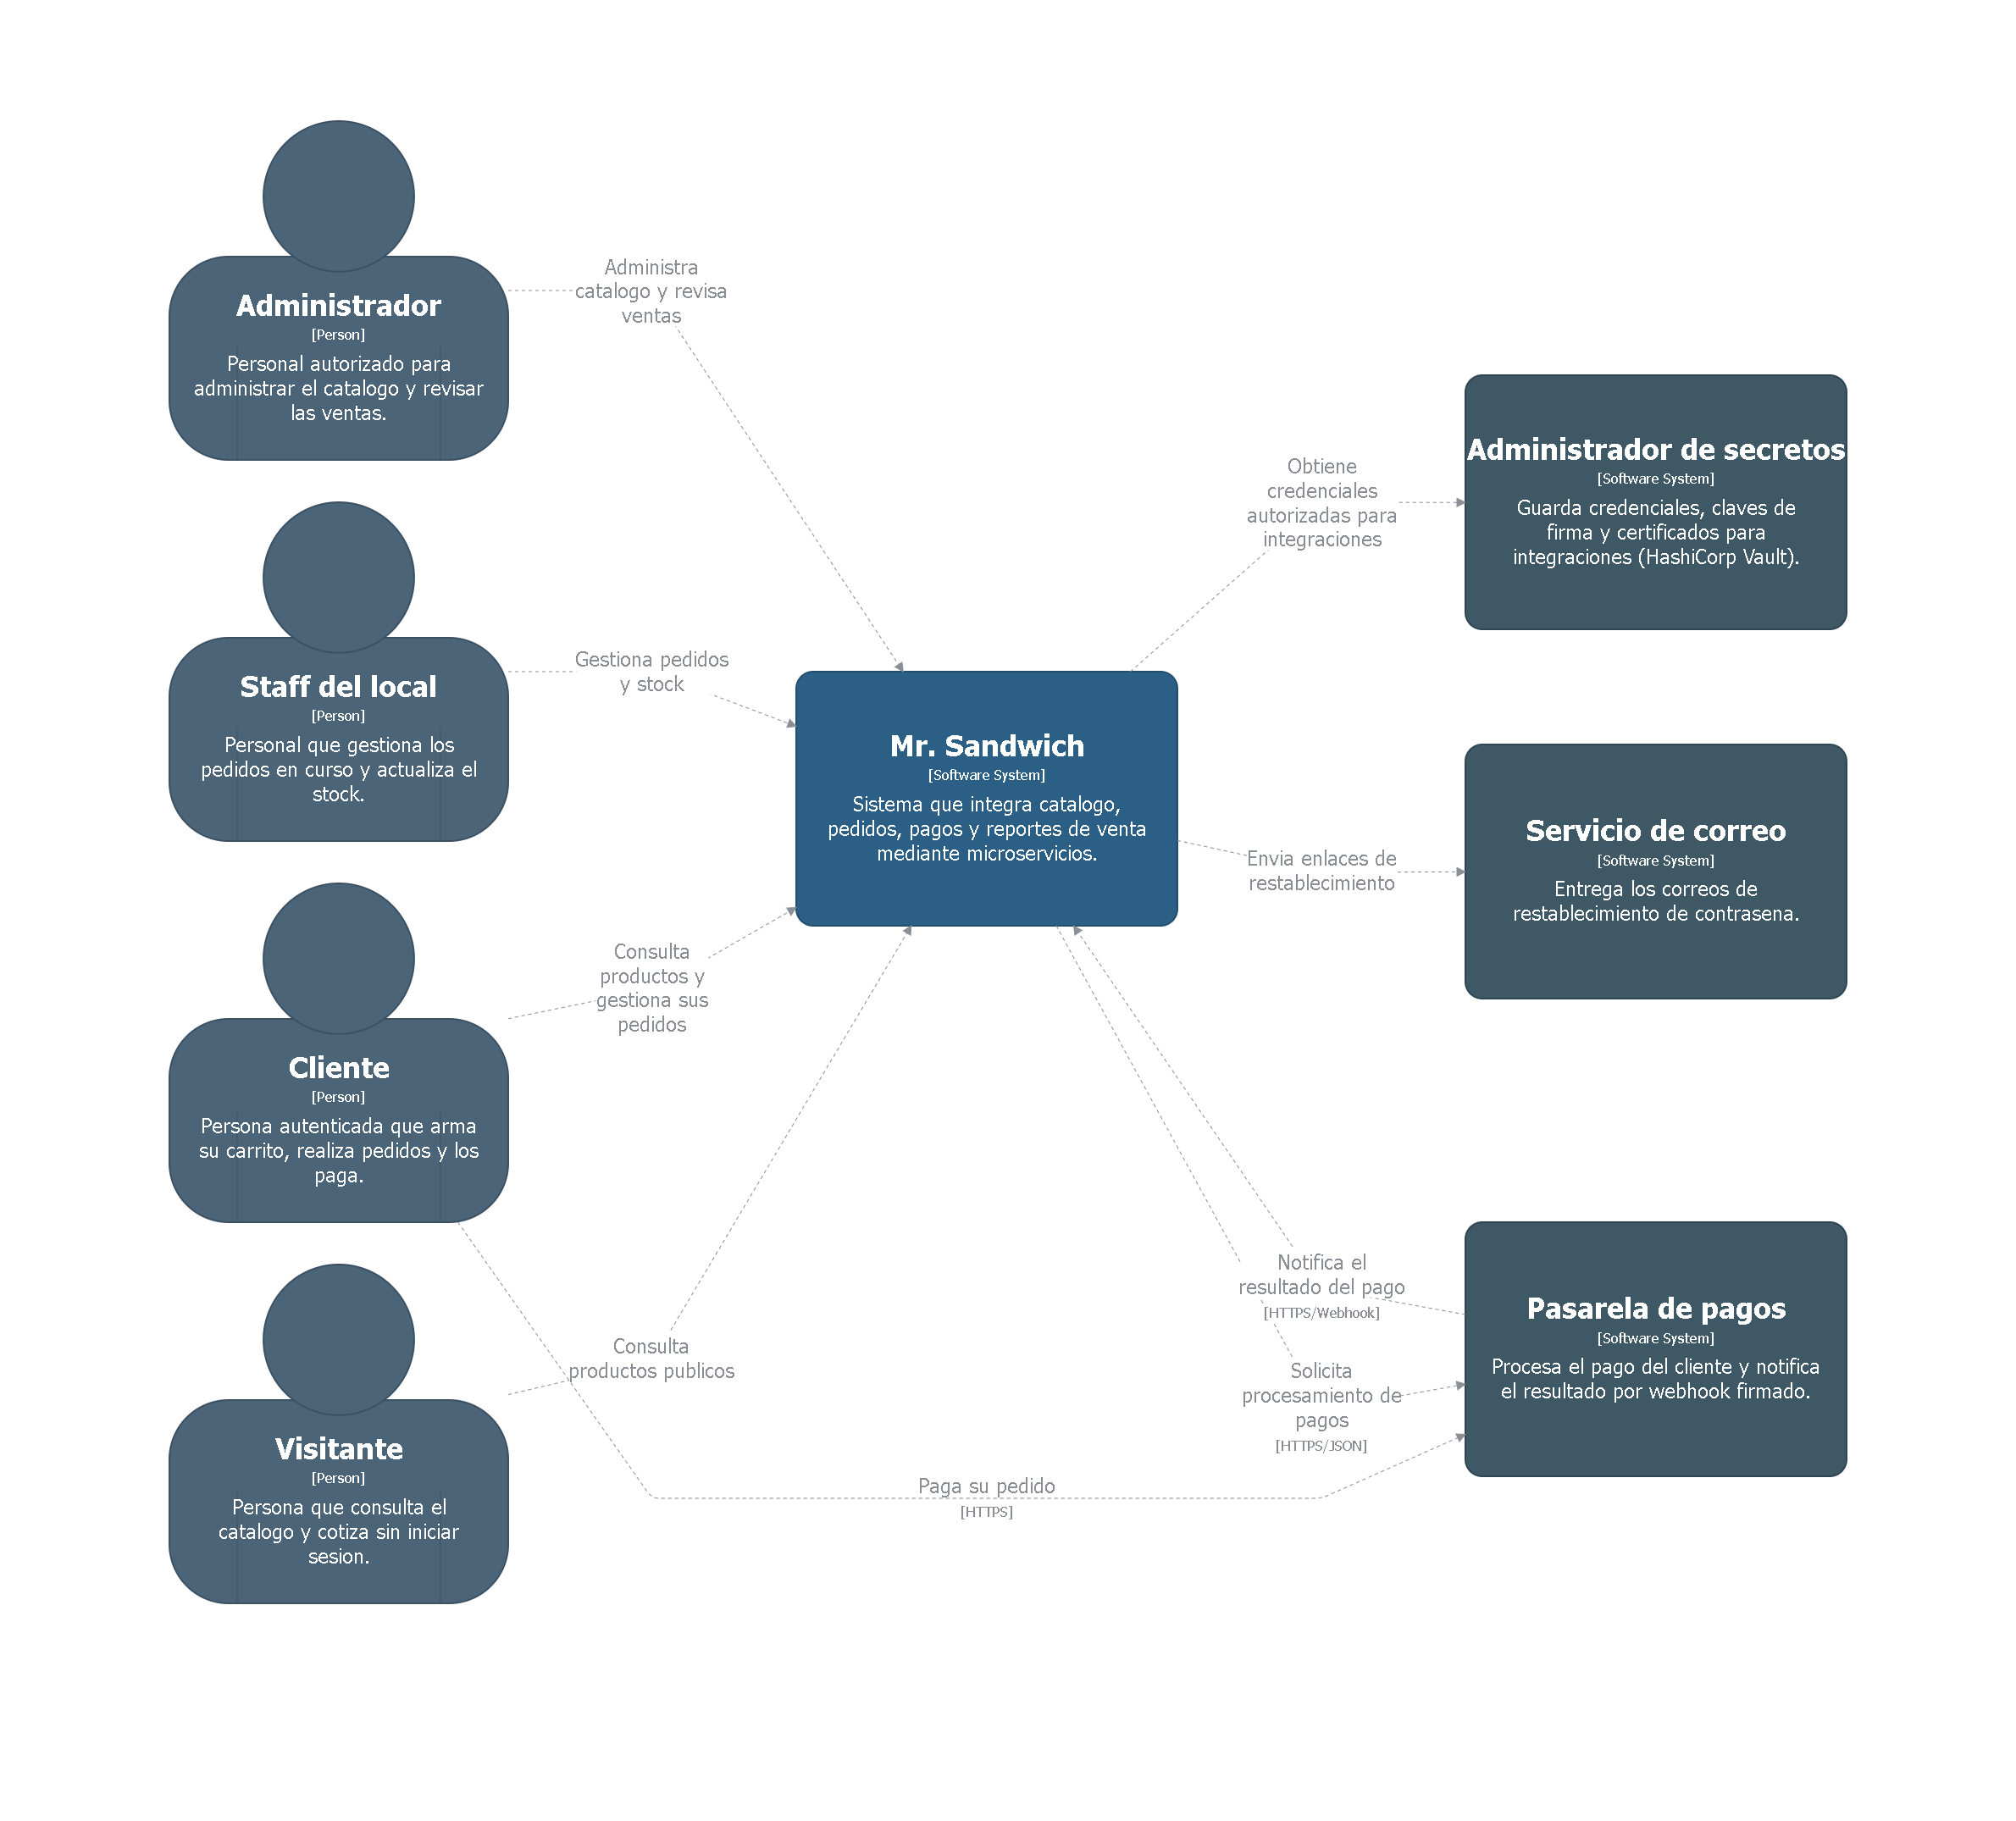
\includegraphics[width=0.85\textwidth,height=0.42\textheight,keepaspectratio]{c4_C1_Contexto.png}
\caption{C1, contexto de Mr. Sandwich}
\end{figure}

\begin{figure}[H]
\centering
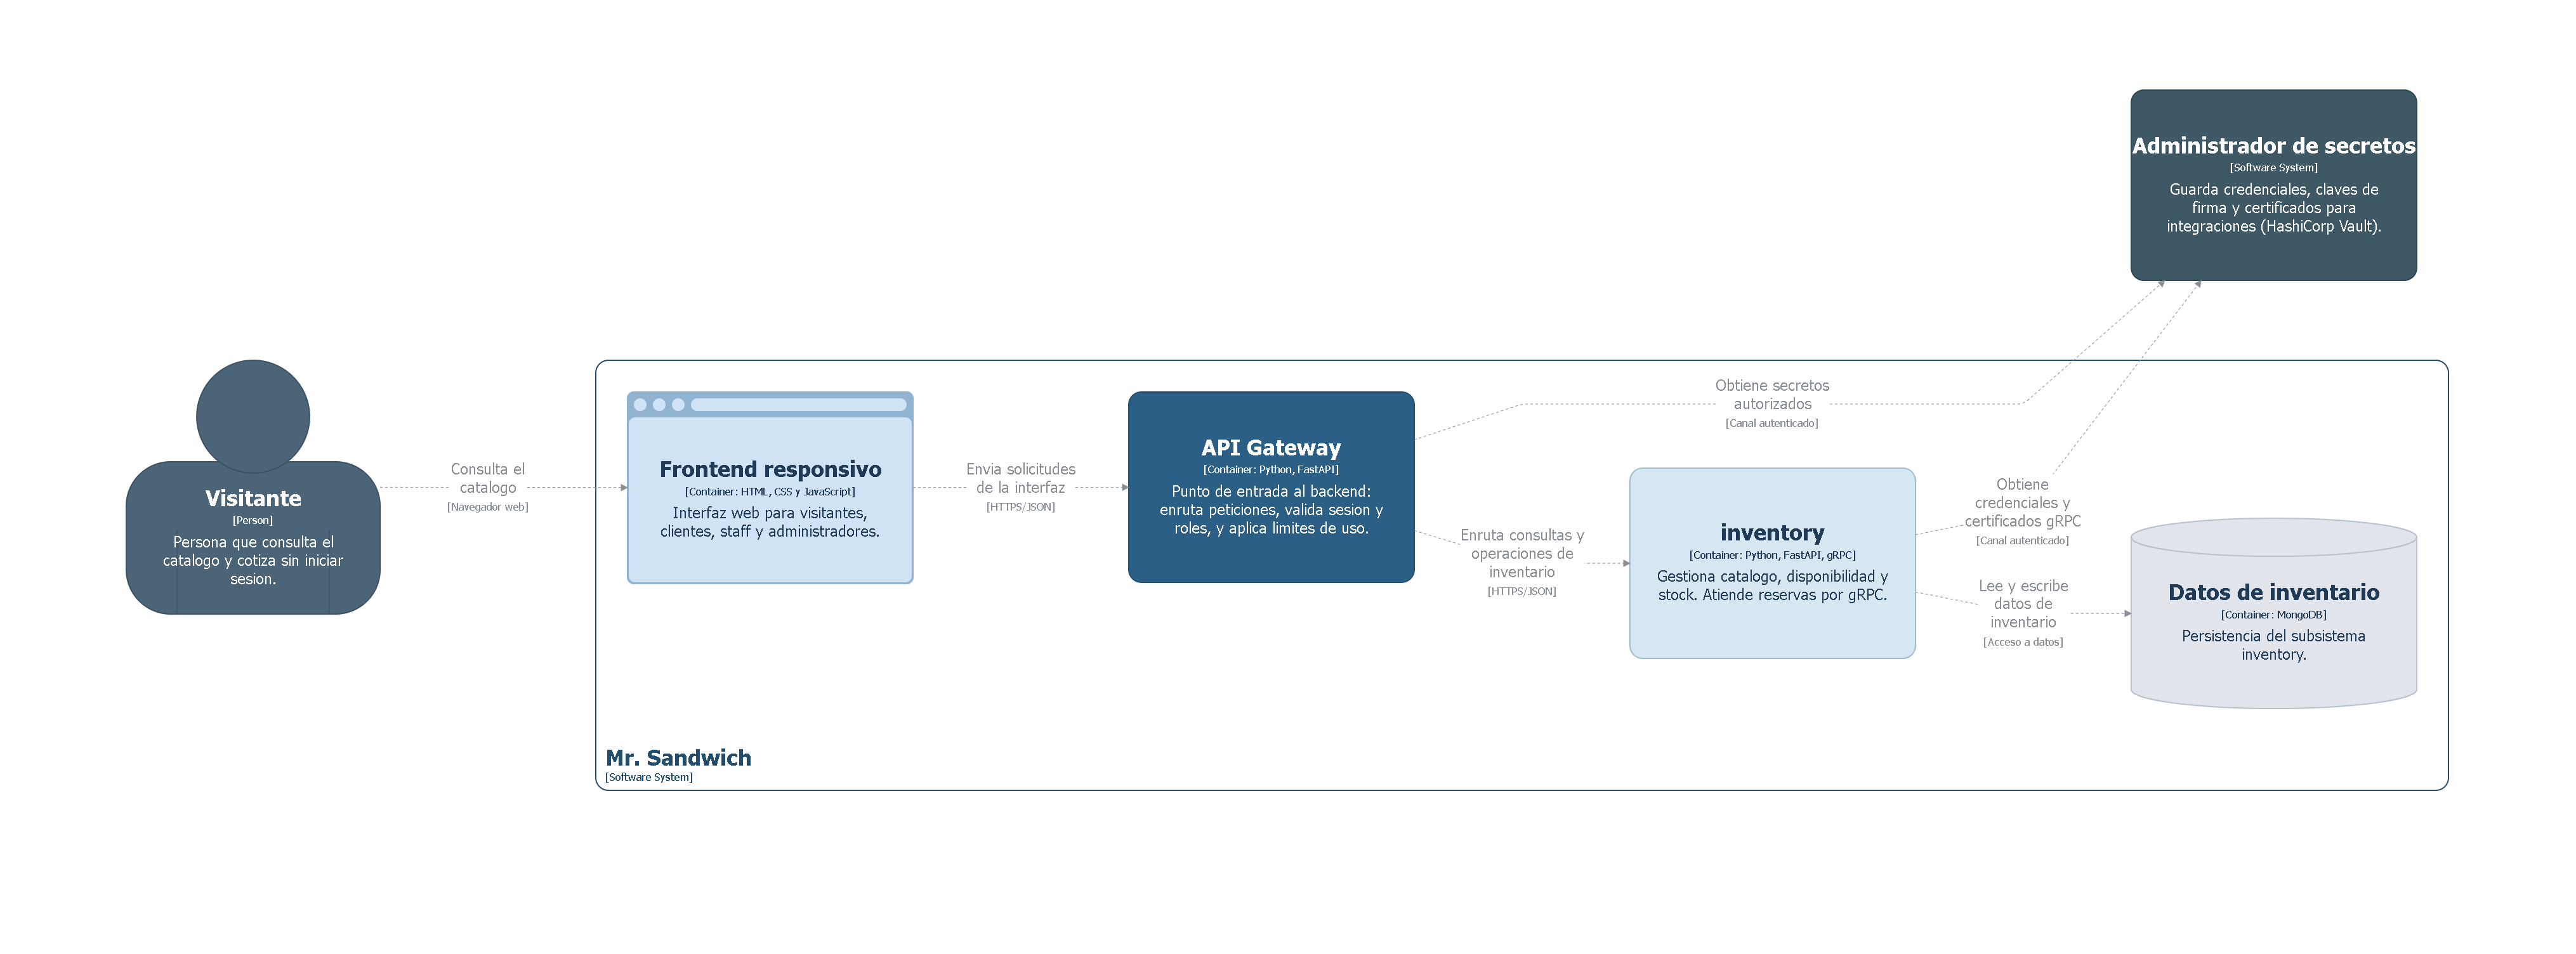
\includegraphics[width=\textwidth,height=0.42\textheight,keepaspectratio]{c4_C2_Consulta_Catalogo.png}
\caption{C2, contenedores que participan en la consulta del catálogo}
\end{figure}

\begin{figure}[H]
\centering
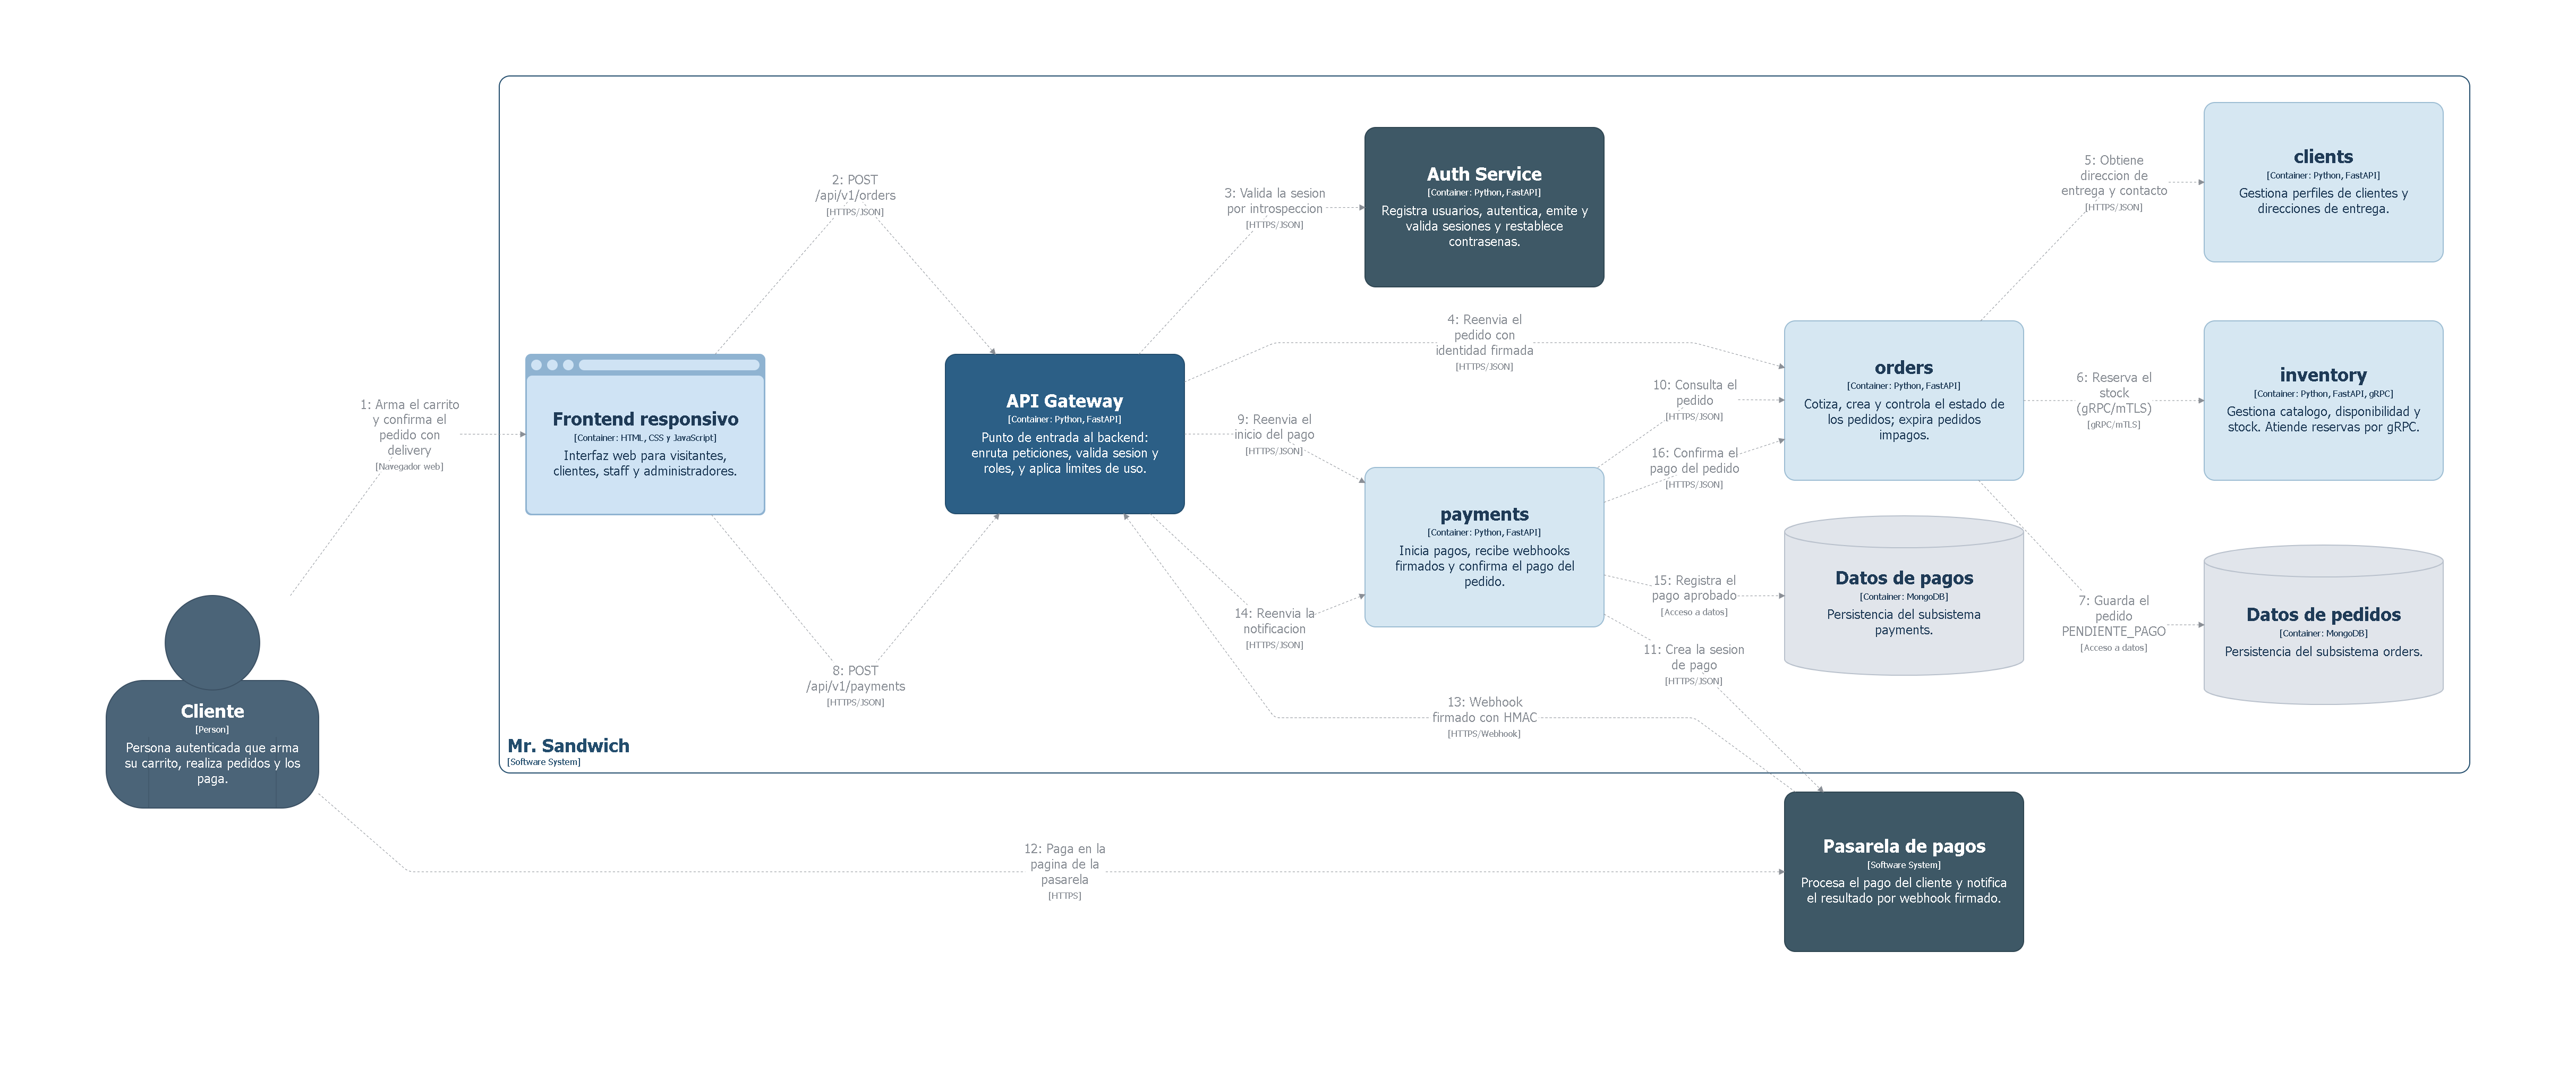
\includegraphics[width=\textwidth,height=0.42\textheight,keepaspectratio]{c4_C2_Registro_Pedido.png}
\caption{C2, secuencia numerada del registro y pago de un pedido}
\end{figure}

\begin{landscape}
\begin{figure}[H]
\centering
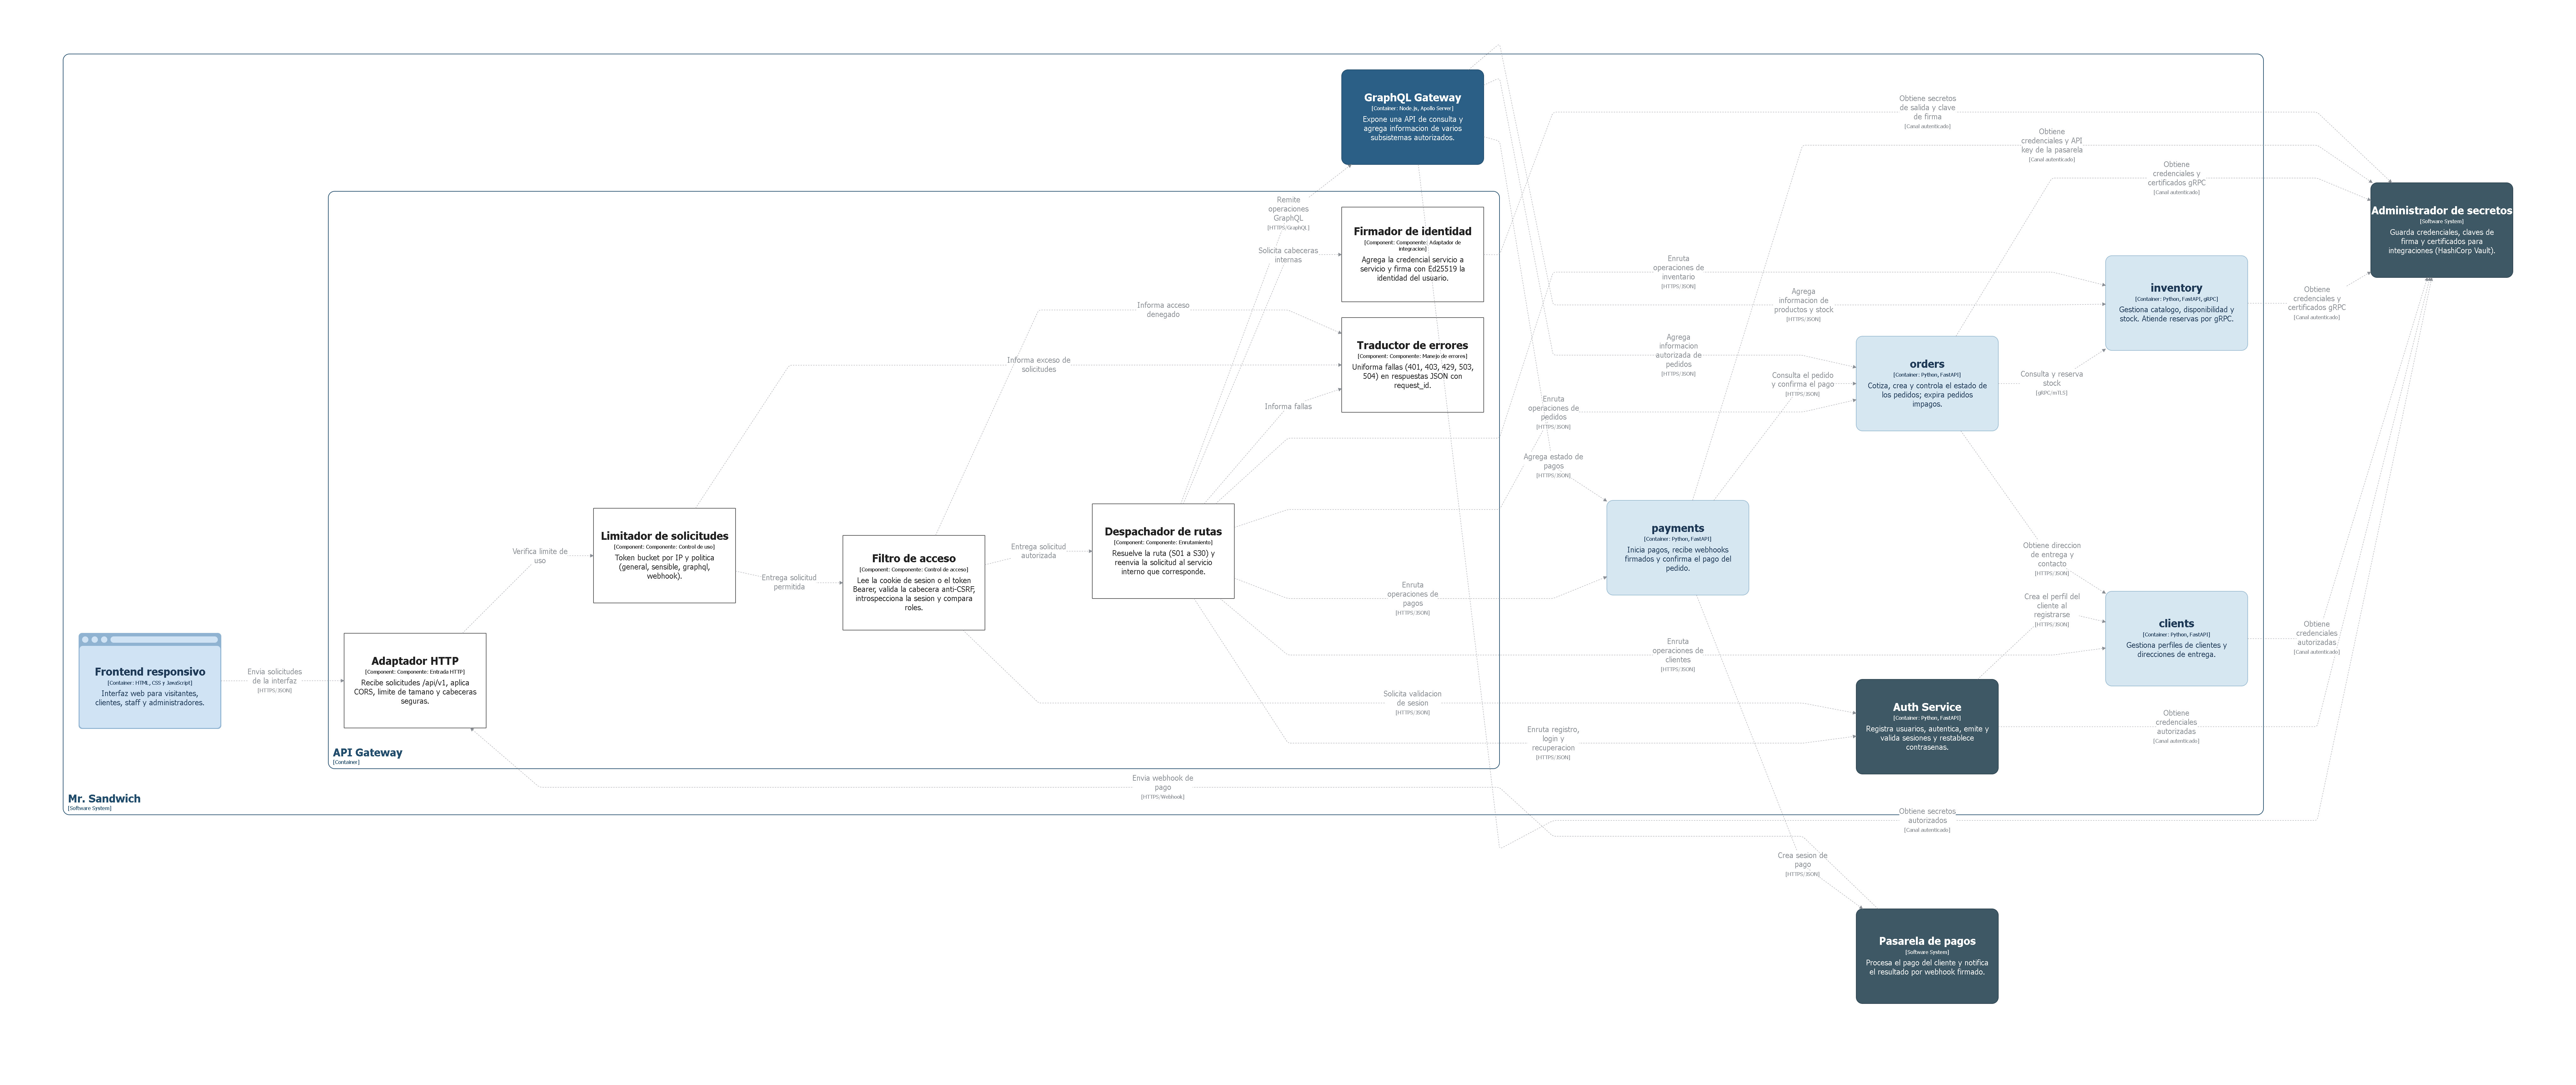
\includegraphics[width=\linewidth,height=0.82\textwidth,keepaspectratio]{c4_C3_API_Gateway.png}
\caption{C3, componentes internos del API Gateway}
\end{figure}
\end{landscape}

\begin{figure}[H]
\centering
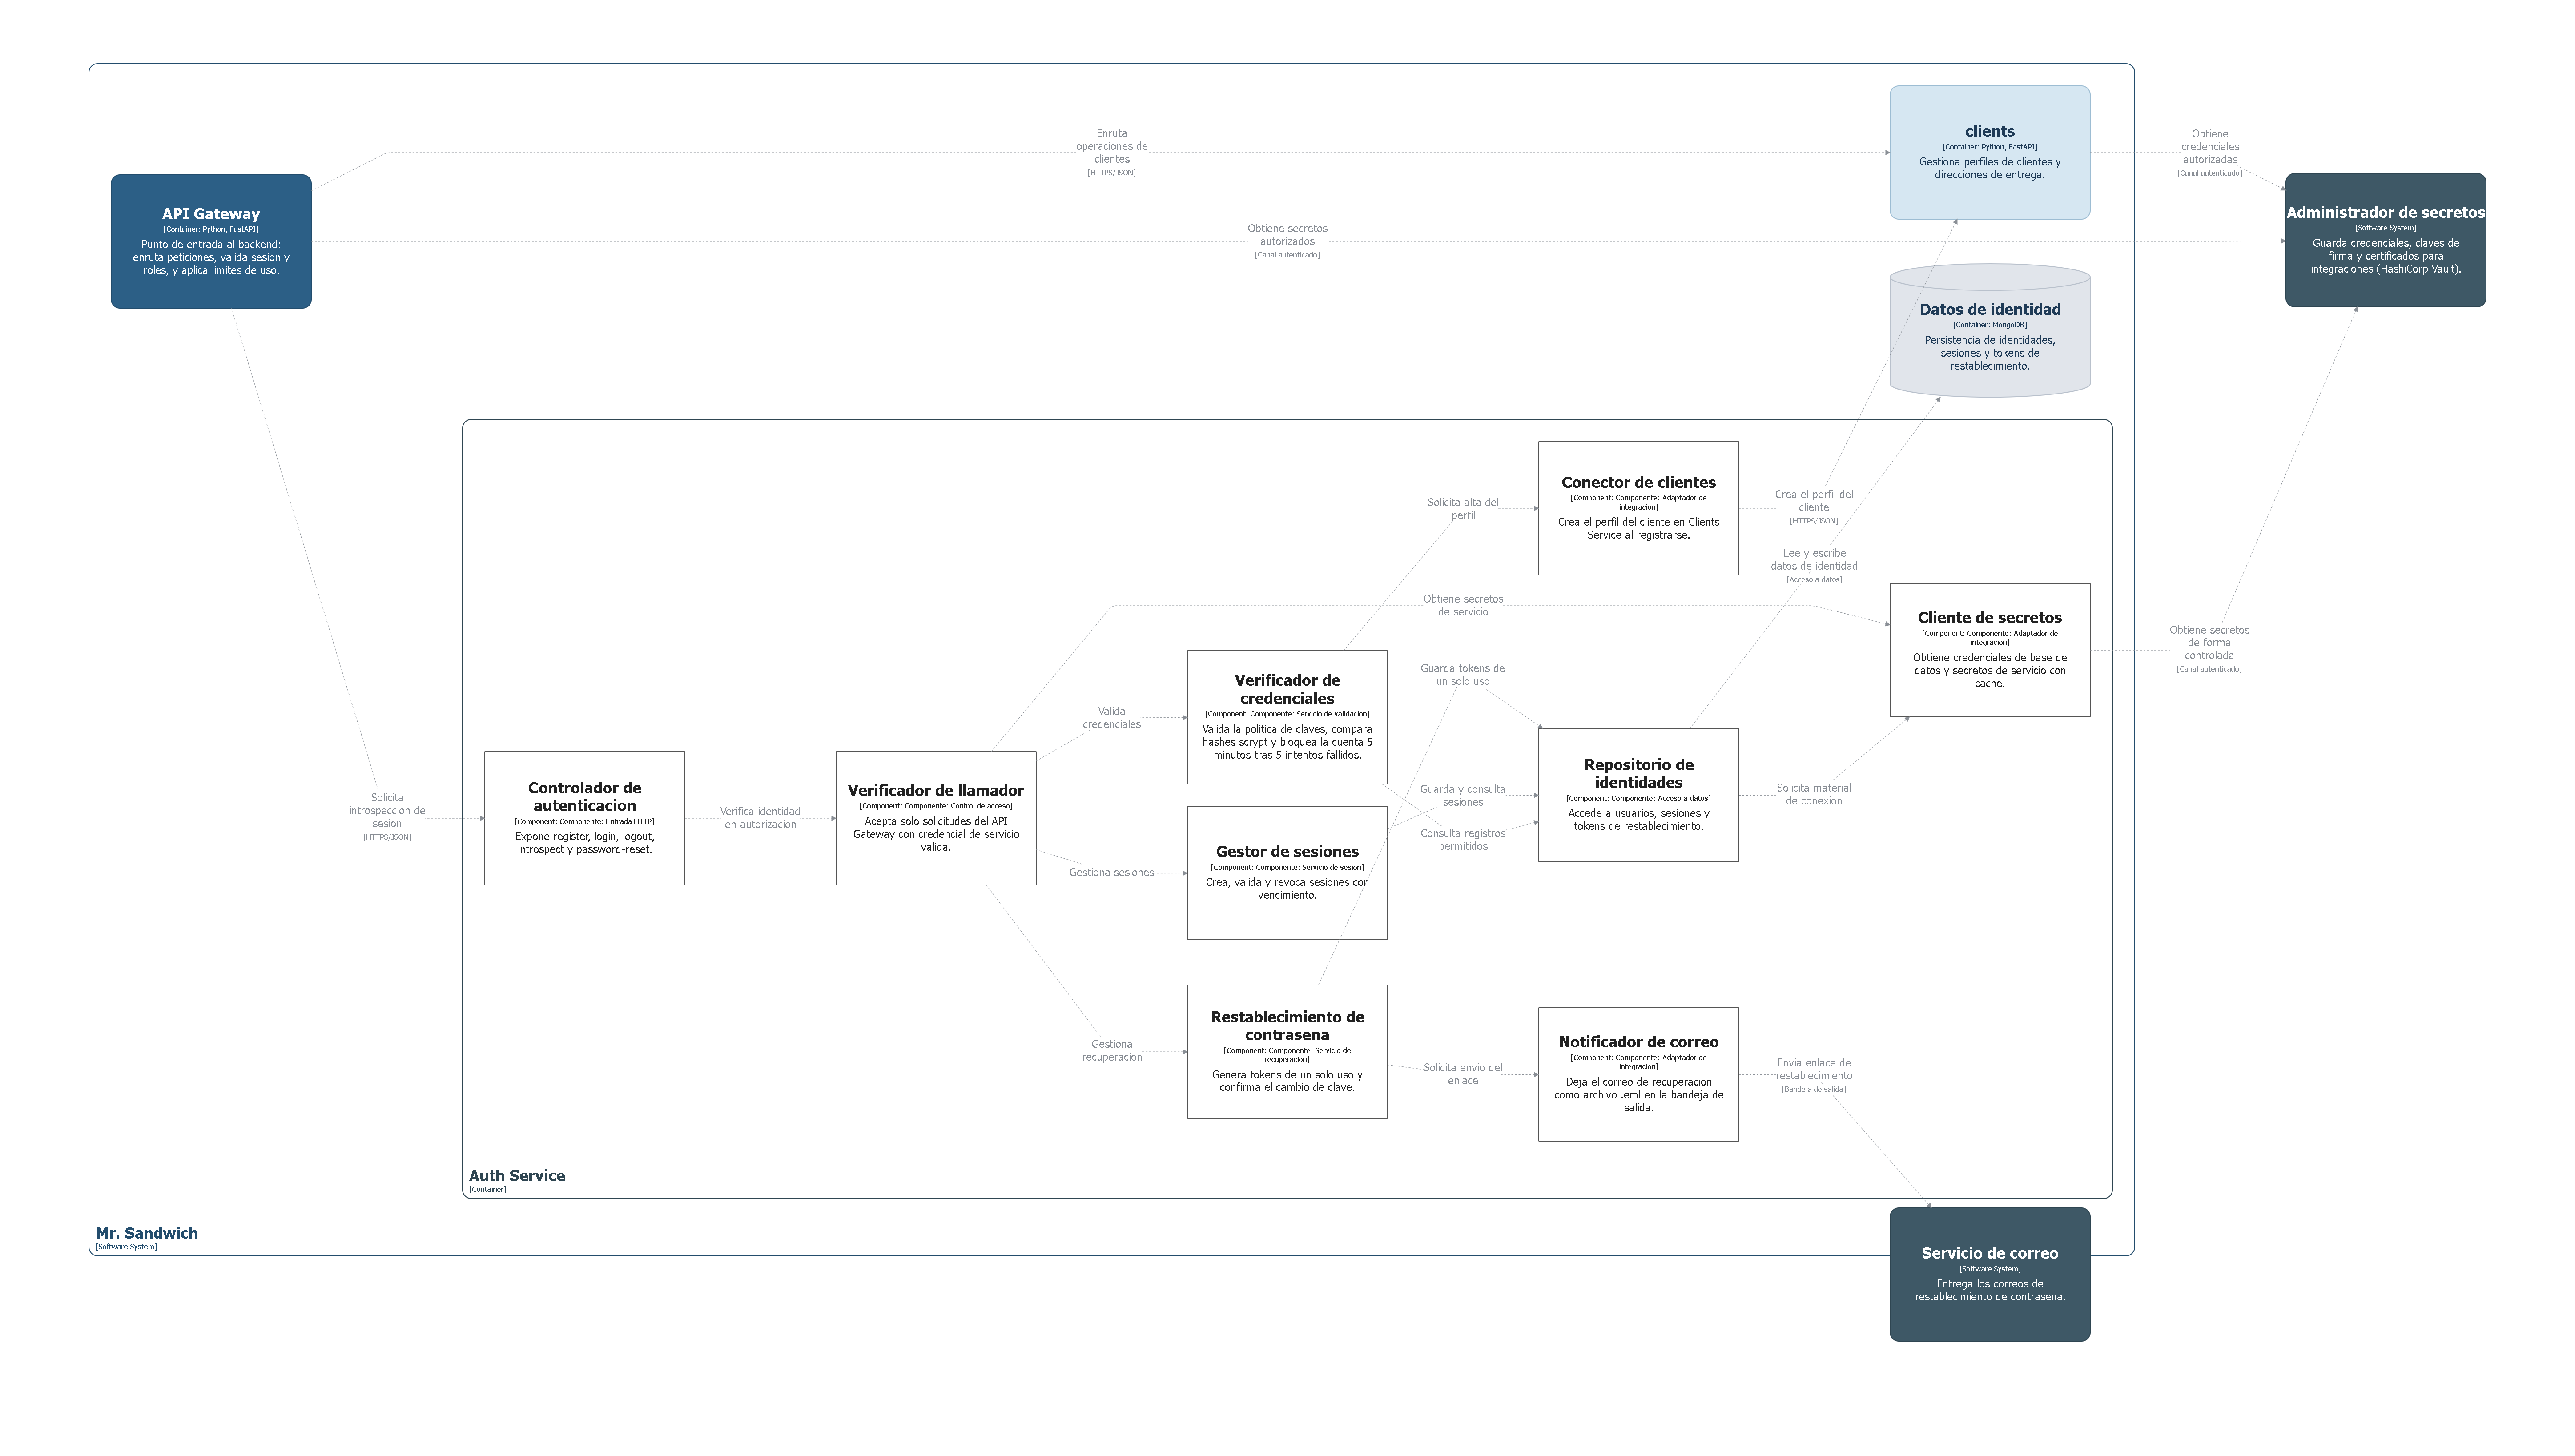
\includegraphics[width=\textwidth,height=0.42\textheight,keepaspectratio]{c4_C3_AuthService.png}
\caption{C3, componentes internos del Auth Service}
\end{figure}

\begin{figure}[H]
\centering
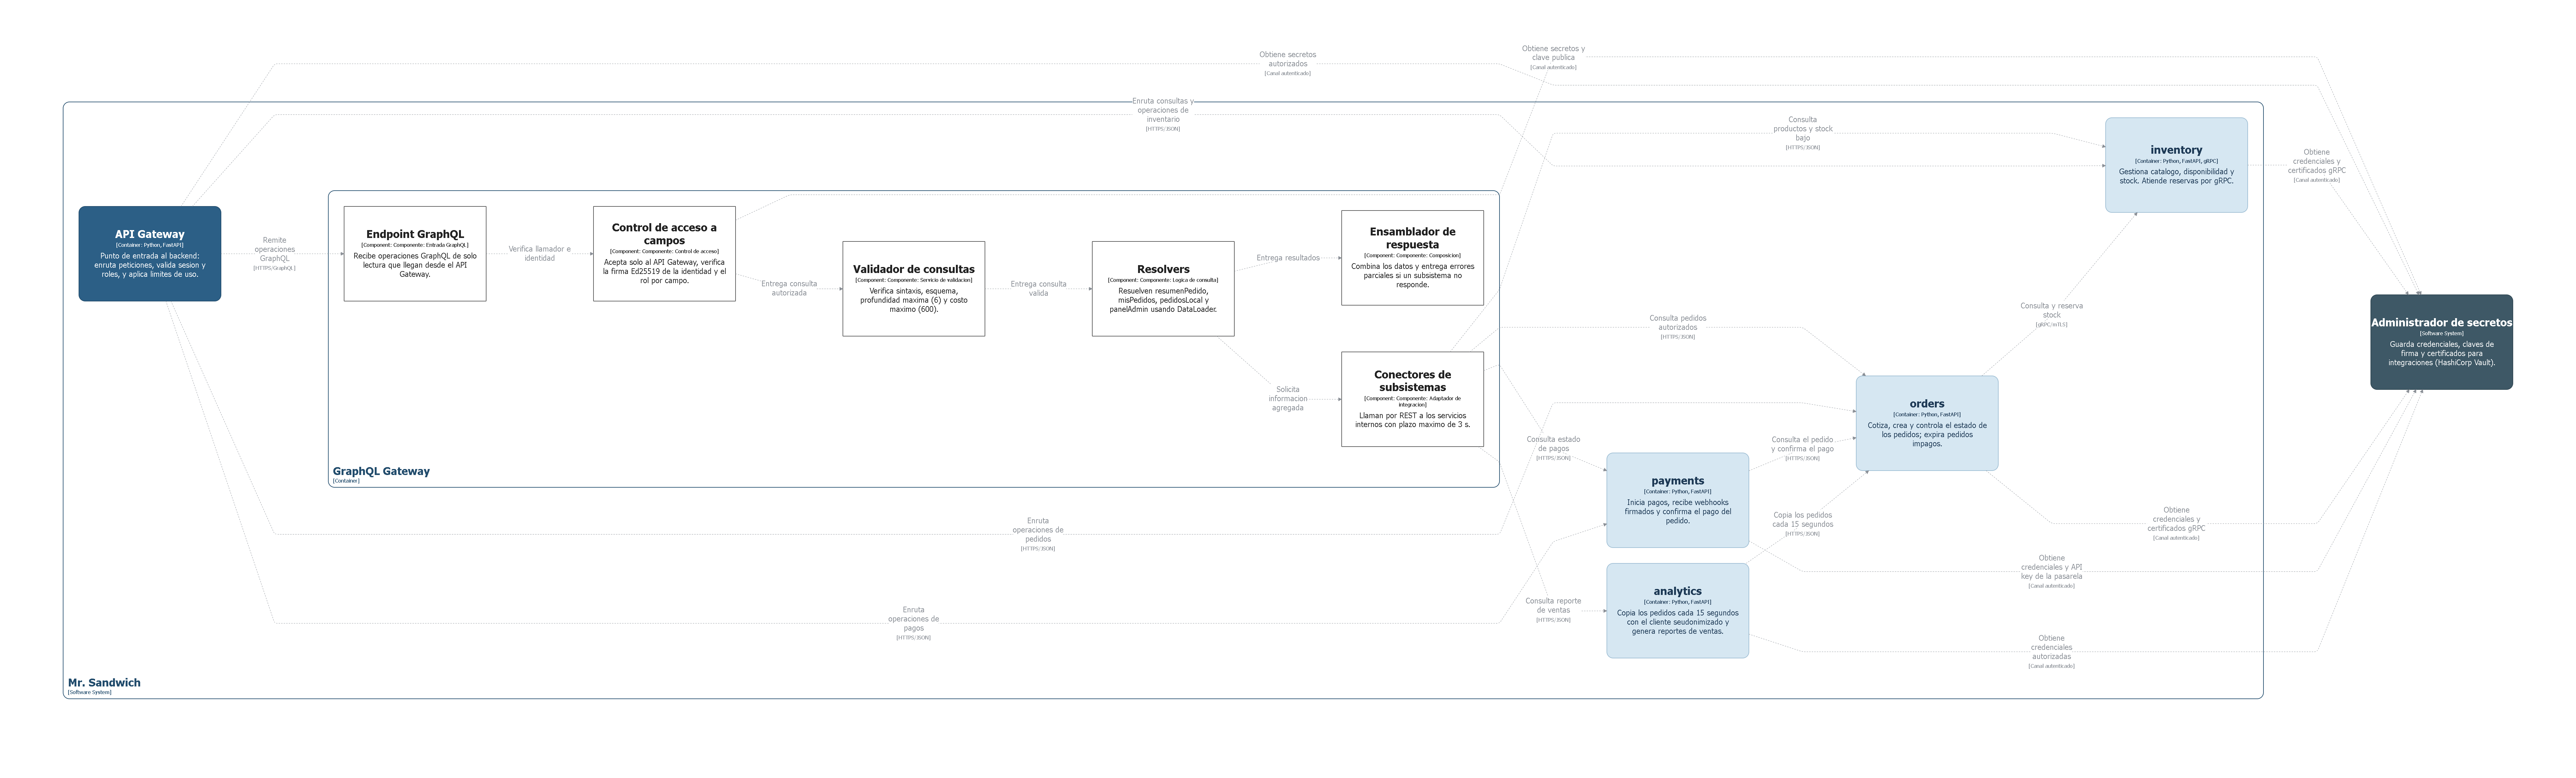
\includegraphics[width=\textwidth,height=0.42\textheight,keepaspectratio]{c4_C3_GraphQL_Gateway.png}
\caption{C3, componentes internos del GraphQL Gateway}
\end{figure}

\end{document}
